% Created 2023-04-03 Mo 17:27
% Intended LaTeX compiler: pdflatex
\documentclass[11pt, twoside]{article}
\usepackage[utf8]{inputenc}
\usepackage[T1]{fontenc}
\usepackage{graphicx}
\usepackage{longtable}
\usepackage{wrapfig}
\usepackage{rotating}
\usepackage[normalem]{ulem}
\usepackage{amsmath}
\usepackage{amssymb}
\usepackage{capt-of}
\usepackage{hyperref}
\usepackage[finnish, interlingua, latin, greek, italian, american, ngerman]{babel}
\usepackage{substitutefont}
\usepackage[a4paper]{geometry}
\usepackage{caption, subcaption, float}
\graphicspath{{./resources/images/}}
\author{Stefan Rohrbacher, Tanja Rumpelmaier}
\date{\today}
\title{DnDisaster\\\medskip
\large 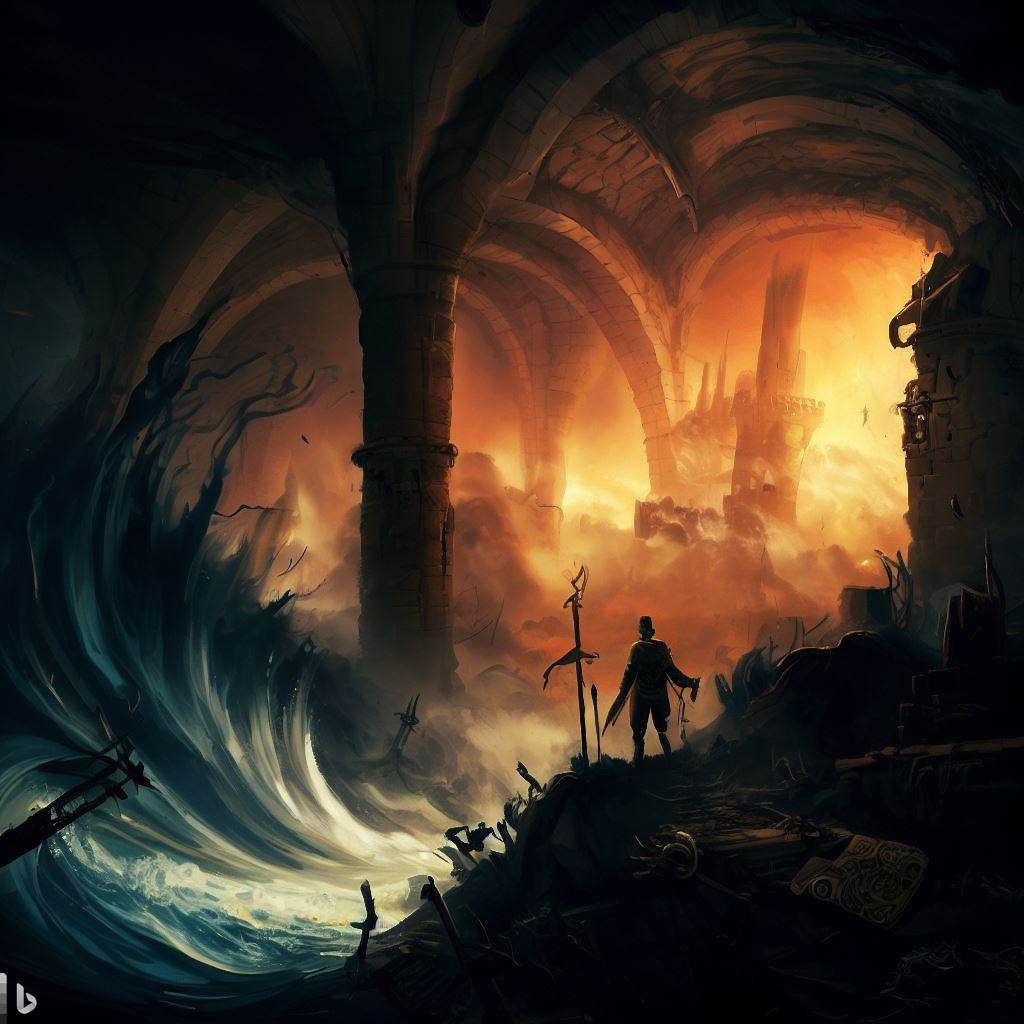
\includegraphics[width=\linewidth]{wallpaper1.jpeg}}
\hypersetup{
 pdfauthor={Stefan Rohrbacher, Tanja Rumpelmaier},
 pdftitle={DnDisaster},
 pdfkeywords={DnD},
 pdfsubject={},
 pdfcreator={Emacs 28.1 (Org mode 9.6.1)}, 
 pdflang={English}}
\begin{document}

\maketitle
\tableofcontents

\newpage

\section{Ideensammlung}
\label{sec:org3d3ccf5}
\begin{itemize}
\item Questidee: Smaragdring von den schwarzen Büchern zurückholen
\item Questidee: Menschen wurden entführt und man soll sie im Lager befreien und die Harpyien besiegen
\item Questidee: Kannibalen-Hexe, die Kinder entführt und in einer Höhle roh verspeist; die Abenteurer müssen sie besiegen und die Kinder - sofern möglich - retten
\item Tal der Schatten (Ork-Dorf)
\item Wüste des Infernos (Süden) mit einer einzelnen Oase
\item Endquest: Das Rätsel um Schloss Schattenhall → Es handelt sich um das Besiegen eines Drachen. Seine Schuppen sind aus Papier sowie Büchern und er hat einen Eisatem
\end{itemize}


\section{Intro}
\label{sec:org328e853}
\begin{itemize}
\item Land: Sommerset (Kesäsarja in Elfisch, Saamnom’raduv in Zwergisch) - Jahr 1250
\end{itemize}

\section{Gebiete}
\label{sec:org00a587f}

\subsection{Wald der Stille (Hiljaisuuden metsä in Elfisch und Prei-Shagāt in Zwergisch)}
\label{sec:org632bcfa}
In diesem Wald leben die magischen Hochelfen. Da man dort fast keine Geräusche hört, wird er Wald der Stille genannt. Es ist windstill, keine Blätter rascheln und man sieht auch keine Tiere. Die Hochelfen haben ebenso eine eigene Sprache und Kultur entwickelt und gehören neben den Halblingen zu den friedliebenden Geschöpfen Sommersets. Sie vermeiden Gewalt und versuchen in Friede und Harmonie zu leben. Sie lieben alles Schöne und wohlwollende und verabscheuen Orks. Dennoch sollte man sie nicht unterschätzen, sie können sich verteidigen, wenn sie müssen und haben eine große Armee.
Es gibt eine versteckte (magische) Elfenstadt Sahira-valaistu in Elfisch und Sal’imanita in Zwergisch - ``die erleuchtete Stadt'', kurz Iluminas, in der Gemeinsprache. Elfen sind Geschöpfe, die keinen Schlaf benötigen, sie bestaunen das Funkeln der Sterne und kommen in der Nacht seelisch zur Ruhe. Ihre Rüstungen und Waffen sowie Kleider sind aus besonderem Metall sowie besonderen Stoff hergestellt. Mondsilber (Kuun’hopeaí) sowie Mondleinen (Kuu’pellava). Die Schönheit ihrer Kleidung und ihrer Stoffe ist einzigartig in Sommersets. An andere Völker bzw. Außenstehenden verkaufen sie ihre Waren jedoch nicht.
Kurz bevor ein böser Waldgeist auftaucht, vernimmt die Gruppe folgendes Gedicht:
\begin{quote}
Über allen Gipfeln
Ist Ruh',
In allen Wipfeln
Spürest Du
Kaum einen Hauch;
Die Vögelein schweigen im Walde.
Warte nur! Balde
Ruhest du auch.
\end{quote}
Die Gruppe kann den Waldgeist nicht besiegen, er fügt ihnen großen Schaden zu, aber niemand stirbt. Gerettet werden sie vom grünen Mann (s. \pageref{gmann}). Sie hören ein Rauschen und einen stürmischen Wind. Der Waldgeist flieht vor Schreck. Ein Faun (s. \pageref{faun}) beobachtet das Geschehen gut versteckt und erklärt der Gruppe, wer das gewesen ist und was das für ein Lebewesen ist. Die Gruppe fragt in die Luft, wie sie sich bedanken kann - einen Luftstoß mit Blättern folgend sehen sie ein Orklager, welches sie beseitigen sollen. Der Faun heilt alle Mitglieder.

\subsection{Wald der Giganten (Jättiläisten’metsä in Elfisch und Prei-Yok in Zwergisch)}
\label{sec:orgebff897}
Dieser Wald befindet sich südlich des Totmannsruh Gebirges. Er besteht lediglich aus Mammutbäumen, Gebüsch, Sträuchern und Lichtungen. In den Mammutbäumen hat ein Waldelfenvolk ihr Dorf errichtet. Sie wohnen in den Baumkronen, haben sie ihr Dorf errichtet. Die runden, spitzen Häuser in den einzelnen Bäumen sind durch Hängebrücken miteinander verbunden. Die Elfen können über Lifte im Inneren der Bäume zum Boden gelangen.
Es gibt viele Tiere, aber auch einige Orklager. Es gibt Hausbäume und Transportationsbäume (ähnlich wie eine Straßenbahn) - die Äste dieser Bäume dienen als Schienen für mechanisch betriebene Wagons zur Transportation von Nahrung, Steinen, Baumaterial etc. Inmitten dieses Walddorfes befindet sich der letzte weiße Mahagonibaum Sommersets, der von allen Elfen als heilig angesehen wird. Da Dinge, die aus der Natur heraus entstehen, an sich keine Namen hat, haben die Waldelfen ihrer Stadt auch keinen Namen gegeben, sie sagen lediglich vom zu Hause (Kotona), wenn sie von ihrem Dorf sprechen.

\subsection{Totmannsruh - Gebirge (Koullut mies lepäa in Elfisch und Msim mnukh in Zwergisch)}
\label{sec:org20ae36b}
Ein riesiges Bergmassiv, ähnlich dem Himalaya, erstreckt sich im Norden des Landes. Es ist das Land des ewigen Winters, bevölkert von Eisbären, Eis-Orks und Eistrollen. Man munkelt, es gäbe auch Eisriesen und Yetis (s. \pageref{yeti}) - wer weiß das schon? Mitten in dieser kargen und unfruchtbaren Landschaft hat sich ein Zwergenvolk tief im Inneren des Berges Kunēsa eingenistet. Sie sind die Nachfahren von Holgar Hammerhand. Ein stolzes und mächtiges Zwergenvolk verfeindet mit den Waldelfen und geschickt bei der Bearbeitung von (Edel-)Steinen. Sture, starrköpfige und eigenbrötlerische Gestalten. Hat man ihr Herz gewonnen, so sind sie loyal bis in den Tod. Sie haben ihr eigenes Schriftsystem (aus Runen), ihre eigene Sprache sowie Kultur im Laufe der Jahrhunderte entwickelt. Sie sind der Meinung, dass sie die Erstgeborenen in Sommerset waren und nicht die arroganten Hochelfen. Mit den Waldelfen sind sie seit dem Krieg des Zorns (Vihan sota in Elfisch und Krôdha di jâga in Zwergisch), im Jahre 500 der Zeitrechnung Sommersets verfeindet. Grund für den Krieg war das Abholzen der weißen Mahagonibäume. Diese Bäume gehen zurück bis zur Entstehung Sommersets - sie waren die ersten Bäume und sind daher für die Waldelfen heilig. Die Zwerge fanden sie besonders stabil und schätzten ihre lange Brenndauer, weshalb sie diese fällten. Dadurch brach ein erbitterter Krieg zwischen den Völkern aus. Bis heute stehen sich diese beiden Völker misstrauisch, fast sogar feindlich, gegenüber.
In dieser Landschaft befindet sich auch der verfallene Tempel Kînesheyn (Kinegrove in Zwergisch, Kinegaròva in Elfisch), mit seinen vielen Räumen und Rätseln gilt er als unlösliches Labyrinth. Obwohl er von einem unbekannten Volk erbaut wurde, ist der Name in allen Sprachen ähnlich. Bis heute ist ungewiss, von welchen Wesen er erbaut wurde. Bis jetzt wurde er noch nie entdeckt - vielleicht eine gute Gelegenheit für unsere Abenteurer? Die Tür wird sich nur Personen reinen Herzens öffnen - ist man erst einmal hineingegangen und findet man den Schatz, so bekommt man den Rosetta Stein Sommersets - wichtige Wörter in Zwergisch, Elfisch und der Gemeinsprache aufgelistet → Lösungswort für die Elfenstadt im Wald der Stille: mīt (Zwergisch) = Ystävä (Elfisch) = Freund.

\subsection{Astrario - Stadt der Menschen}
\label{sec:orgaa09020}
Eine mittelalterlich inspirierte Stadt, bewohnt von Menschen (hauptsächlich). Am Stadtrand leben die ärmeren Bürger: Mägde, Bauern, manche Handwerker und Bettler. Je näher man ins Stadtzentrum vordringt, desto reicher werden die Leute. Über der Stadt ragt eine imposante Burg aus weißem Marmor. Diese dient als Wohnsitz des Regenten, aber auch als Universität der menschlichen Magier. Die Stadt hat die üblichen Probleme der Menschen: Armut, Rassismus, Sklaverei, Klassengesellschaft. Individuen der anderen Völker haben sich in der Stadt angesiedelt und leben entweder in Ghettos oder sie werden aufgrund ihrer außerordentlichen Fähigkeiten in den Bereichen der Menschen geduldet. Die Magie forscher ``Etheri'' (s. \pageref{etheri}) der Universität haben im Verlies der Burg eine gefährliche Entdeckung/Experimente gemacht (Bol'gith). Menschen sind das jüngste Volk in Sommerset und versuchen regelmäßig den anderen Völkern gewaltsam Ressourcen und Land zu entwenden.

In der Universität leben nicht nur die Gelehrten, sondern auch sogenannte Buchlinge (s. \pageref{buchling}) (Kreaturen von Walter Moers), kleine zyklopartige Lebewesen, die nur für Bücher leben und alle Bücher eines Autors auswendig lernen.

Buchlinge sind zwar nach ihren Autor:innen benannt, aber nicht korrekt, sondern in der Form als Anagramm.
Buchlingsnamen: Ydro Blorn, Heidler von Clirrfisch, Freiherr von Dillschic, Ali Aria Ekmirrner, Estrakos, Zank Frakfa, Dr. Fidemus Grund, Sanotthe von Rhüffel-Ostend, Ojahnn Golgo van Fontheweg.

Die Buchlinge wandern zwar in der Bibliothek und in der Stadt frei herum, schlafen aber in der geheimen Bibliothek der Universität. Dort lesen sie lediglich die Bücher ihrer Autor:innen. In Astrario gibt es nicht nur einen Markt, sondern auch einen Buchmarkt sowie einen Schwarzbuchmarkt – das Pendant zu einem Schwarzmarkt. Unsere Abenteurer entdecken diesen per Zufall. Dort wird ihnen heimlich folgender Notiz zugesteckt:
\begin{quote}
In tiefen, kalten, hohlen Räumen
Wo Schatten sich mit Schatten paaren
Wo alte Bücher Träume träumen
Von Zeiten, als sie Bäume waren
Wo Kohle Diamant gebiert
Man weder Licht noch Gnade kennt
Dort ist’s, wo jener Geist regiert
Den man den Schattenkönig nennt.

Getürmt aus Buch auf Buch
Verlassen und verflucht
Gesäumt von toten Fenstern
Bewohnt nur von Gespenstern
Befallen von Getier
Aus Leder und Papier
Ein Ort aus Wahn und Schall
Genannt Schloss Schattenhall.

Ihr Abenteurer seid weit gereist und wohl bekannt Findet und erledigt das Monster und ihr werdet fürstlich entlohnt werden.
\end{quote}

Ein Buchling wird währenddessen auf die Abenteurer:innen aufmerksam und möchte sich ihnen anschließen. Falls die Gruppe das verneinen sollte, kann er mit Tränen und süßem Aussehen überzeugen. Es handelt sich um den kleinen Buchling Ojahnn Golgo van Fontheweg, der nur Bücher von Johann Wolfgang von Goethe liest. Er ernährt sich, indem er Bücher liest und sie rezitiert. Er ist jedoch nicht der begabteste Lerner und kann sich seinen Text nur schwer merken. Deswegen hat er wenige Freunde und ist auch nicht so beliebt. Im Kampf ist er generell nicht so nützlich, er taugt lediglich dazu, irgendwelche Zitate von berühmten Personen zu rezitieren. Ojahnn hat dennoch viel Wissen über die Geschöpfe und Geschichte Sommersets. Er kann euch viel zu Orten und Lebewesen erzählen.

Zu seinen Zitaten gehören:
\begin{enumerate}
\item \texttt{Fantasie ist wichtiger als Wissen, denn Wissen ist begrenzt. - Albert Einstein}
\item \texttt{Sein oder Nichtsein; das ist hier die Frage - William Shakespeare}
\item \texttt{Alle wollen die Welt verändern, aber keiner sich selbst. - Lew Nikolajewitsch Tolstoi}
\item \texttt{Es irrt der Mensch, solang er strebt – Goethe} →  wichtigstes Zitat für ihn
\item \texttt{Wege entstehen dadurch, dass man sie geht. - Franz Kafka}
\item \texttt{Nur die Oberflächlichen kennen sich selbst. - Oscar Wilde}
\item \texttt{Das Leben wird vorwärts gelebt und rückwärts verstanden. - Søren Kierkegaard}
\item \texttt{Nicht der Mensch hat am meisten gelebt, welcher die höchsten Jahre zählt, sondern derjenige, welcher sein Leben am meisten empfunden hat. - Jean-Jacques Rousseau}
\item \texttt{Viel mehr als unsere Fähigkeiten sind es unsere Entscheidungen, die zeigen, wer wir wirklich sind. - J.K. Rowling}
\item \texttt{Wo sich eine Türe schließt, öffnet sich eine andere. - Moliére}
\item \texttt{Es ist besser ein einziges kleines Licht anzuzünden, als die Dunkelheit zu verfluchen. - Konfuzius}
\item \texttt{Cogito ergo sum - René Descartes}
\end{enumerate}

Unterhalb von Astrario befinden sich Katakomben, die einem Labyrinth ähneln. In diesem Leben die träumenden Bücher - eine bestimmte Rasse von Buch, das fühlen, denken und vor allem träumen kann. Träumende Bücher haben eine große Anziehungskraft, sind aber leicht mit Feuer zu bekämpfen. Es gibt auch die Schattenbücher - sogenannte Schwarze Bücher - wer sie öffnet, wird verflucht und erleidet einen Giftschaden. In diesem Labyrinth lebt auch eine Sphinx(p. \pageref{sphinx}). Er ist sehr weise, aber einsam. Wenn man eine Quest für ihn erledigt - bekommt man als Belohnung einen Schatz (Edelsteine).

\subsection{Die Weitluftebene (Laaja-alainen ilma in Elfisch, Khyāl-Tchōm in Zwergisch)}
\label{sec:org62055af}
Liegt in der Mitte des Gebiets und grenzt im Norden an den Wald der Giganten und im Osten an den weißen Hafen. Diese Ebene ist von sanften, grünen Hügeln geprägt. Es gibt viel Weidefläche und vereinzelte kleine Dörfer. Es handelt sich um ein sehr fruchtbares Gebiet, das von Halblingen bewohnt und bewirtschaftet wird. Halblinge sind das geselligste Volk von Sommerset und stehts mit allen Völkern - bis auf Orks, Trolle etc. befreundet. Halblinge arbeiten als einfache Landwirte, betreiben Tauschhandel und gelten als zufriedene und gutmütige Lebewesen. Durch ihr diplomatisches Geschick haben sie es geschafft, all die Jahre neutral und verschont von Krieg zu bleiben. Die Hauptstadt der Weitluftebene ist Immerwind (Everwindin in Elfisch, Khyāl-cheanich in Zwergisch).

Die Weitluftebene wird von verschiedenen Flüssen durchkreuzt, in denen allerhand Gefahren lauern.

\subsection{Eversonn - der weiße Hafen}
\label{sec:orgcc5a81f}
Eversonn ist der einzige Hafen in ganz Sommerset, obwohl er in jeder Sprache einen Namen hat, wird er von allen Völkern lediglich der weiße Hafen genannt. Grund dafür ist eine Bauart aus weißem Marmor, verziert mit Mondsilber. Wer sich hier auf den Weg in die unendlichen Meere machte, kehrte nie wieder zurück. Es wird vermutet, dass auf der anderen Seite des Meeres der Urkontinent allen Lebens auf dieser Erde ist - Gondwana (Góndàvaná in Elfisch und Hkaud-veana in Zwergisch). Wie die Lebewesen auf Sommerset kamen, ist nicht bekannt. In Eversonn leben lediglich Tempeldiener der weißen Sterne - Elfen, Halblinge und Menschen. Sie tragen lange, weiße Roben mit Kapuzen und verehren die Sterne und den Wind. Ihrer Meinung nach wurde die Erde von Stella, auch genannt Mutter Stern, und Vento, auch genannt Vater Wind, erschaffen. Sie glauben fest daran, dass eines Tages die Seelen aller in Sommerset lebenden Geschöpfe nach Gondwana zurückkehren und mit einem großen Knall in der Ewigkeit vergehen werden. Sie sind davon überzeugt, dass sie durch Stella und Vento mittels eines leisen Knalles erschaffen wurden und, dass sich dieser Kreislauf letztendlich wieder schließen müsse.

In Eversonn befindet sich auch die größte Bibliothek Sommersets - die Bibliothek zu den Sternen. Dabei handelt es sich um ein viereckiges Gebäude mit zwiebelähnlichen, meterhohen Türmen in den Ecken. In der Mitte des Hofs steht die 30 m hohe Bibliothek - ein gigantischer Turm des Wissens. Dieser ist von runden Räumen und deckenhohen Bücherregalen geprägt. Wissen aller Völker, in unterschiedlichsten Sprachen, ist hier anzutreffen. Jedoch nicht nur Wissen der frohen Geschöpfe, sondern auch jenes der dunklen Gestalten (Orks etc.). Das Gebäude beherbergt aber nicht nur eine Bibliothek, sondern auch eine Zitadelle, in der die Weisen Sommersets ausgebildet werden. Nur die weisesten und ältesten Elfen geben hier ihr Wissen weiter. Die älteste Elfin ist Thranal (Thranala) - sie ist über 1.200 Jahre alt. Gerüchten zufolge war sie die erste Elfin, die Sommerset betrat. Sie verneint dies jedoch stets. Sie lebt ein sehr zurückgezogenes Leben, ist aber bereit, anderen Wesen Hilfe zuteilen bzw. Rat zu erteilen.

\subsection{Höhle der Erinnerung (Muistojen luola in Elfisch und Yādā di guphā in Zwergisch)}
\label{sec:org70d75b4}
In dieser Höhle müssen sich die Abenteurer ihrer schlimmsten Erinnerung stellen - kann entweder ausgedacht sein oder wirklich passiert sein. Sie müssen sich diese Situation vor Augen halten und sie auf einem anderen Weg lösen als sie es damals gemacht haben (z. B.: Mobbingerfahrung - nicht mit Hass oder Vergeltung reagieren, sondern mit Liebe und Güte, z. B. Täter umarmen und einsehen, dass er aus einer Unsicherheit/Unzufriedenheit etc. handelt).
Sofortiges Lvl-Up nach dem Bestehen der Höhle + Schatz, wenn geschafft - jeder Charakter bekommt eine Waffe, die um 2 Schadenspunkte stärker ist.

\subsection{Tal der Schatten (Varjojen laakso in Elfisch und Saidō di ghātī in Zwergtisch)}
\label{sec:org403ef01}
Das Tal liegt nördlich der Wüste und ist von Gebirge umgeben. Dadurch kann gibt es dort kein Sonnenlicht, geschweige denn Mondlicht. Die Wesen, die dort ihr Unwesen treiben sind, alle sehr hässlich, missraten und sehen allesamt gruselig aus. Cliffhänger: Sie sind eigentlich total liebe Lebewesen und werden umsonst gefürchtet. Ihr Aussehen und die Gerüchte rund um das Tal schützen sie vor Feinden. Die Abenteurer müssen es schaffen, friedlich mit ihnen zu kommunizieren und sie nicht anzugreifen. Dann bekommen sie als Dankeschön Geschenke der Bewohner:innen - Rüstungsteile mit besseren Verteidigungswerte für jede Rasse.
Im Tal der Schatten befindet sich aber auch ein Ork-Dorf. Die Bewohner:innen des Tals bitten die Gruppe darum, die Orks zu vertreiben.

\subsection{Infernowüste}
\label{sec:org30ce7ed}

\newpage

\section{Bestiarium}
\label{sec:org04d59c4}
Alle Lebewesen respektieren und fürchten - nicht zu Unrecht - den grünen Mann. Es gibt ihn schon so lange es Leben gibt und alles Leben wird mit ihm erlöschen.
In jedem Gebiet gibt es Trolle, Orks, Zyklopen und Riesen.

\clearpage

\subsection{Nomaden und Omnipräsente Wesen}
\label{sec:orgebbc9aa}
\subsubsection{Me und Me\label{meme}}
\label{sec:orgd52ea3c}
2 ungleiche Zwillinge, ein Halbelf und ein Gnom betreiben gemeinsam einen fahrenden Handel. Sie sind der festen Überzeugung Geschwister zu sein obwohl sie sich kein bisschen ähnlich sehen. Gezogen wird ihr Wagen von 2 Haflinger-Pferden Lo und Rd.
\begin{figure}[H]
\centering
\caption{Die Händler Me und Me}
\label{fig:meme}
  \begin{subfigure}{0.5\textwidth}
    \centering
    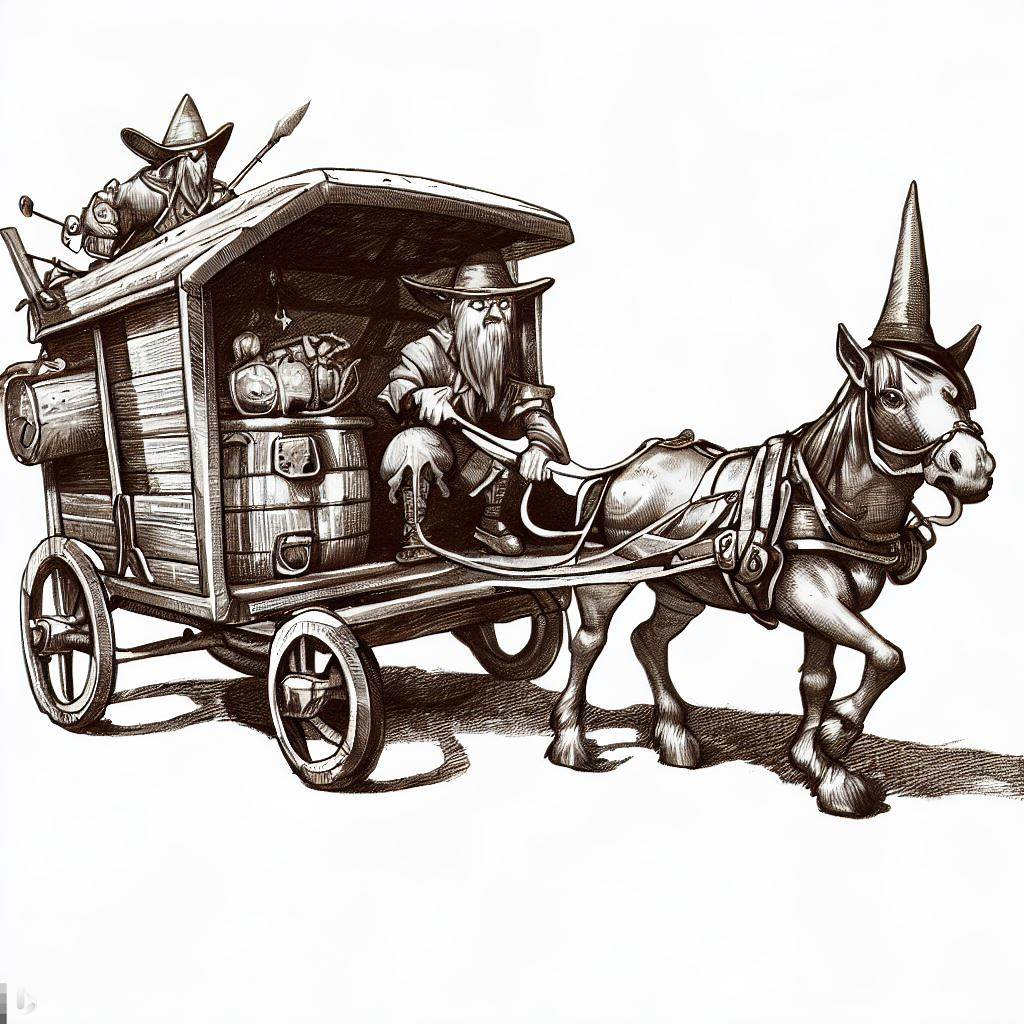
\includegraphics[width=0.99\linewidth]{meme.jpeg}
    %\caption{Ethera}
  \end{subfigure}
\end{figure}

\newpage

\subsection{Wald der Stille}
\label{sec:orgf8bacb6}
\subsubsection{Faune\label{faun}}
\label{sec:orga749114}
Gutmütige, humorvolle Wesen - halb Ziege, halb Mensch; wenn man sie zum Essen einlädt, helfen sie einem; sind Abenteurern sehr freundlich gesinnt und haben einen guten Sinn für Humor;
\begin{figure}[H]
\centering
\caption{Faune}
\label{fig:faun}
  \begin{subfigure}{0.3\textwidth}
    \centering
    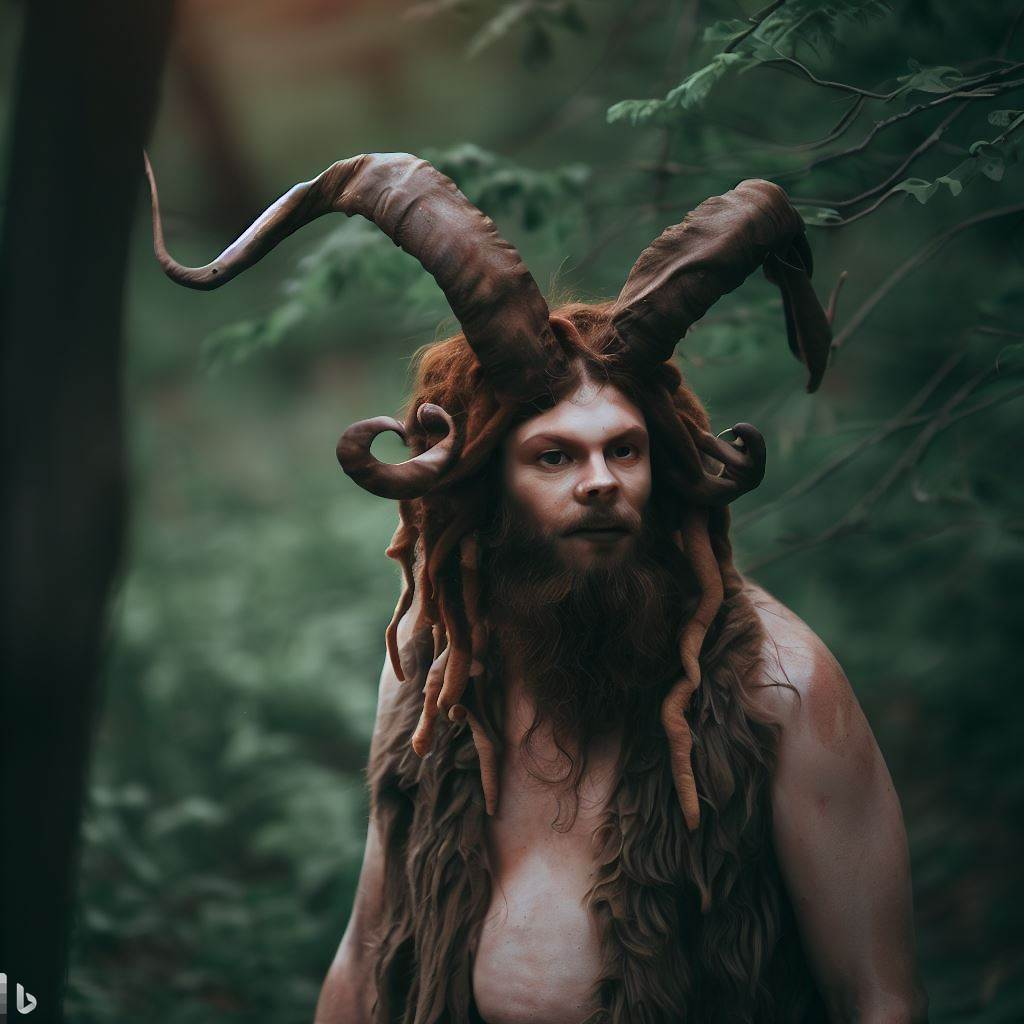
\includegraphics[width=0.99\linewidth]{faun1.jpeg}
    %\caption{Faun}
  \end{subfigure}%
  \begin{subfigure}{0.3\textwidth}
    \centering
    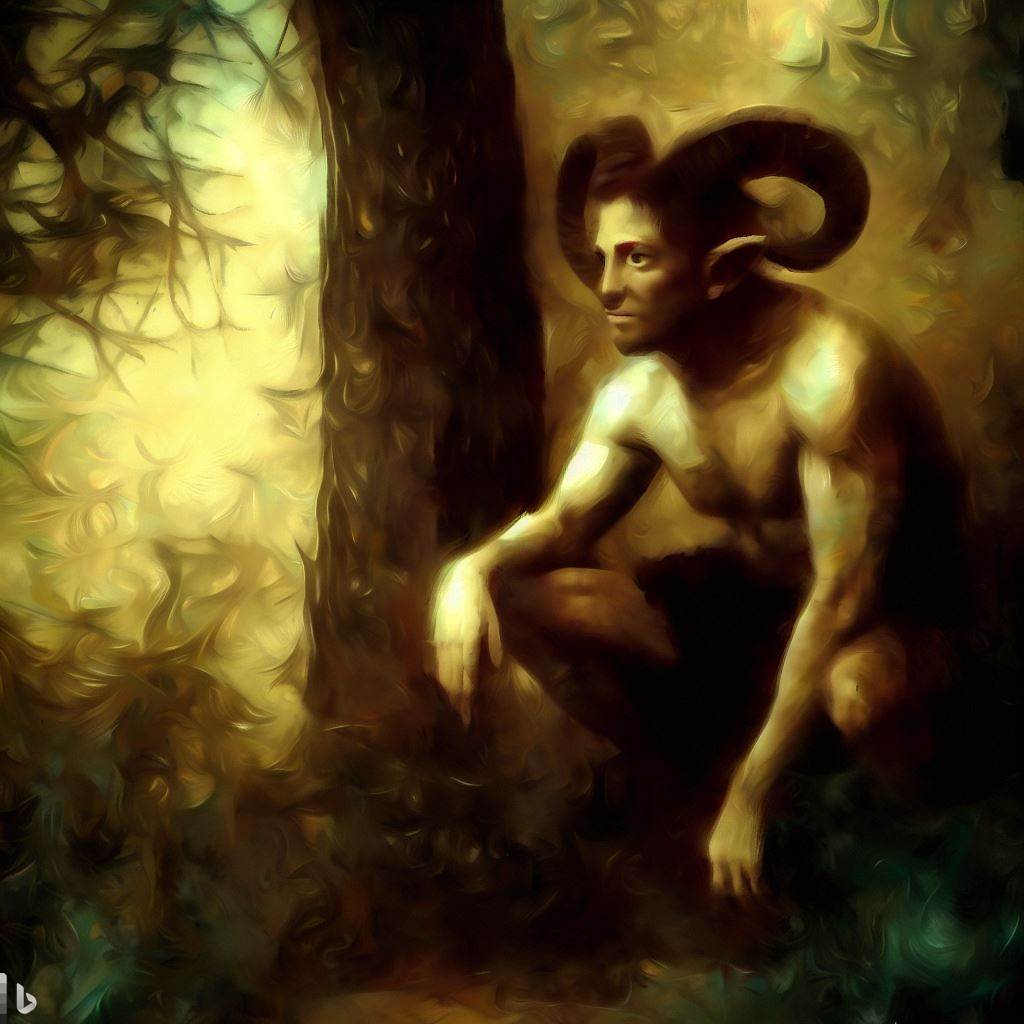
\includegraphics[width=0.99\linewidth]{faun2.jpeg}
    %\caption{Faun}
  \end{subfigure}%
  \begin{subfigure}{0.3\textwidth}
    \centering
    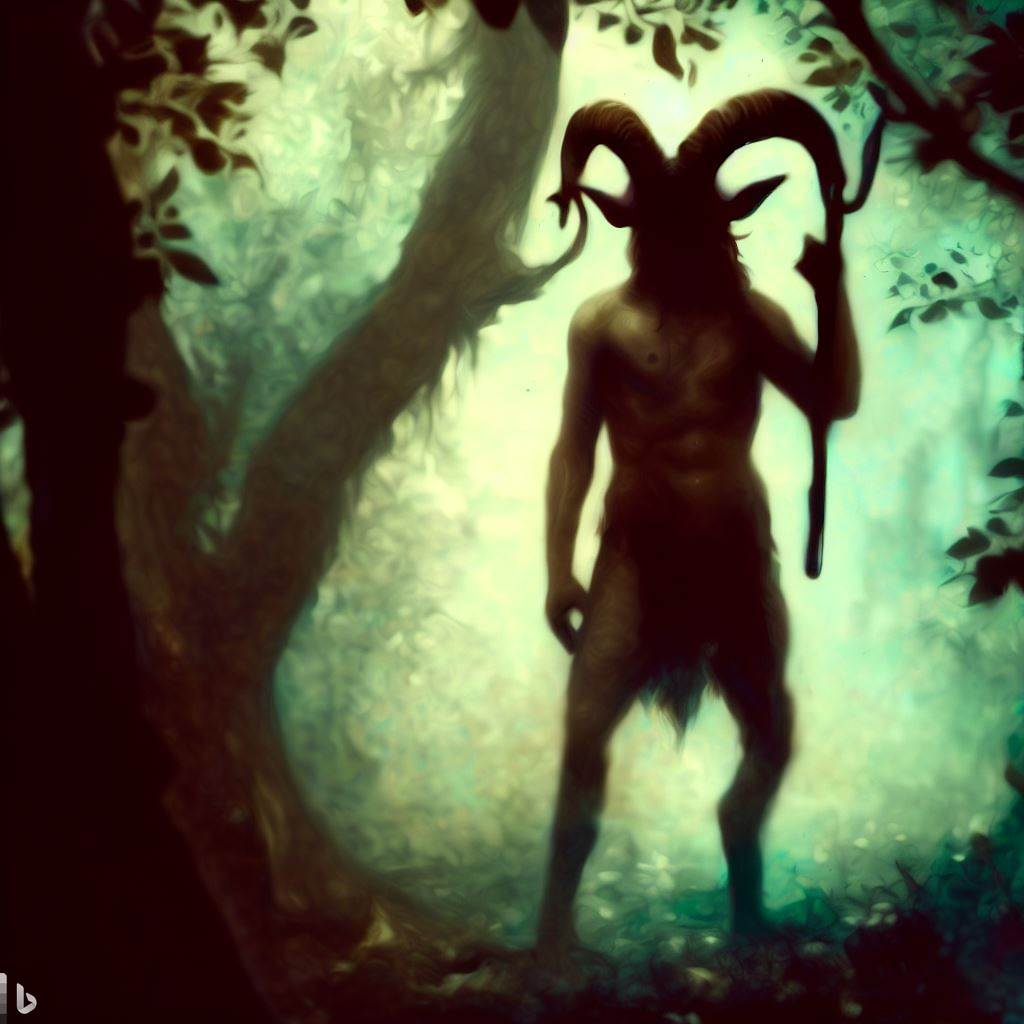
\includegraphics[width=0.99\linewidth]{faun3.jpeg}
    %\caption{Faun}
  \end{subfigure}%
\end{figure}

\subsubsection{Der grüne Mann\label{gmann}}
\label{sec:orga8043ad}
er existiert schon seit dem Anfang allen Dingen, niemand weiß, wie er aussieht, bis auf Thranal - sie behaupte, sie habe ihn schon einmal gesehen; es handelt sich um einen mächtigen Geist; er ist komplett grün, sein Haupt belaubt; er ist die lebenspendende Kraft des Pflanzenreiches und im ganzen Land bekannt - er wird auch als der Mann des Waldes bezeichnet; wenn er in der Nähe ist, hört sich das Rascheln der Bäume so an als “spräche der Wald”; er ist der Retter in der Not, zeigt sich nie, heilt aber verwundete;
\begin{figure}[H]
\centering
\caption{Der grüne Mann}
\label{fig:gmann}
  \begin{subfigure}{0.3\textwidth}
    \centering
    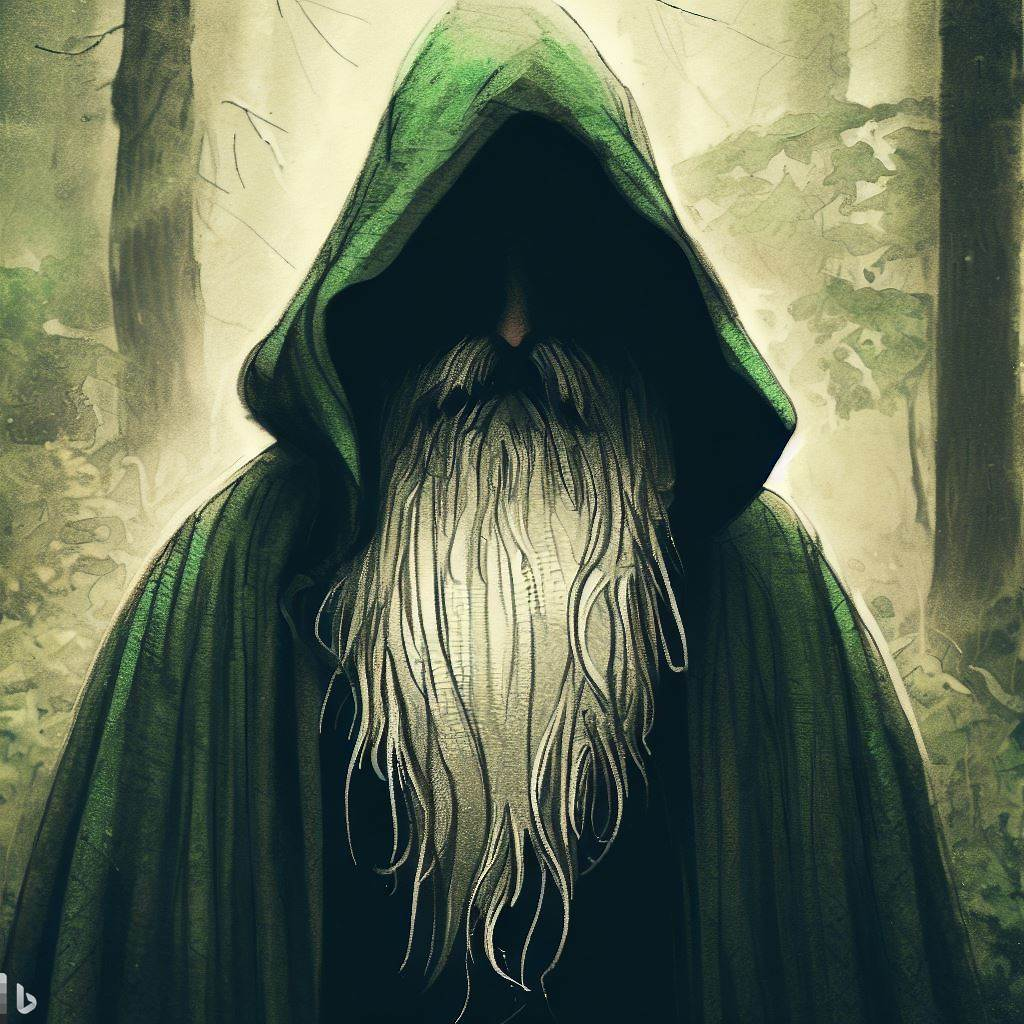
\includegraphics[width=0.99\linewidth]{gmann1.jpeg}
    %\caption{Ethera}
  \end{subfigure}%
  \begin{subfigure}{0.3\textwidth}
    \centering
    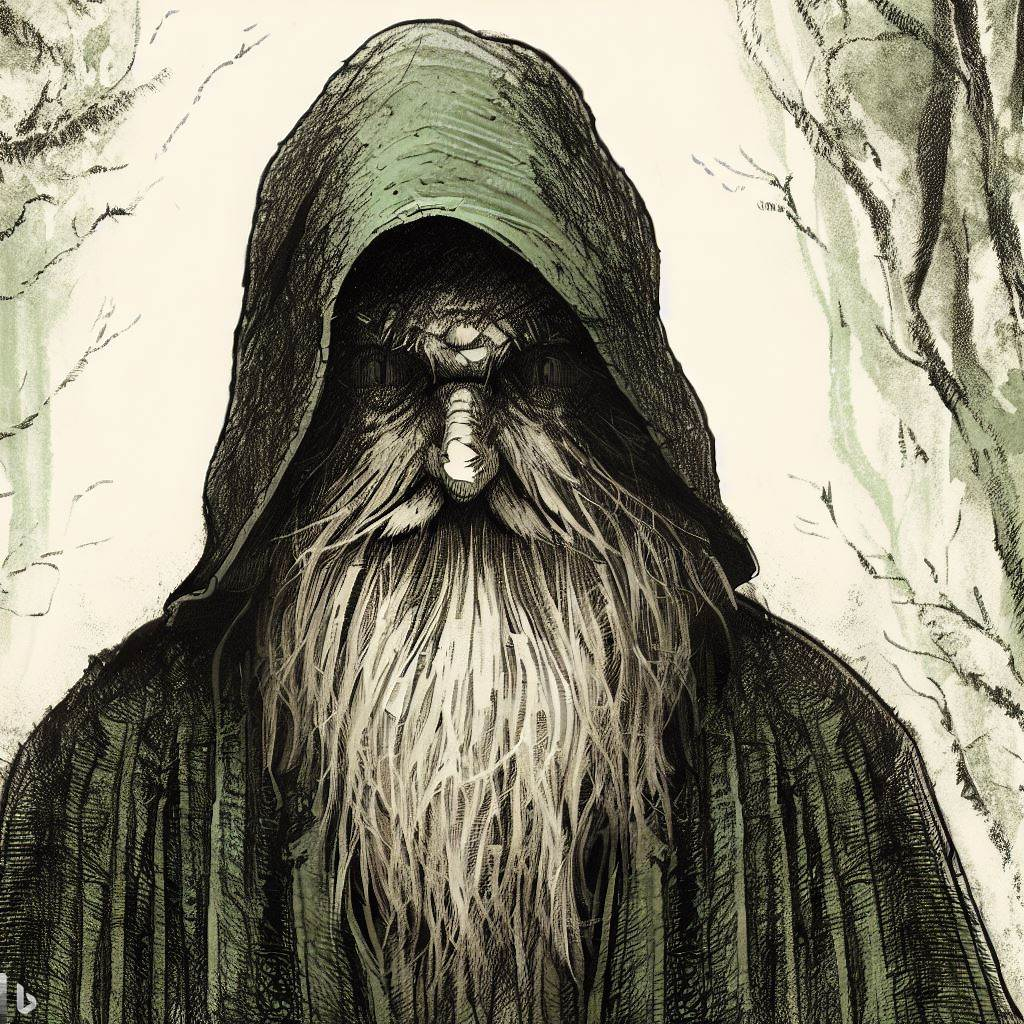
\includegraphics[width=0.99\linewidth]{gmann2.jpeg}
    %\caption{Etherus Meister}
  \end{subfigure}%
  \begin{subfigure}{0.3\textwidth}
    \centering
    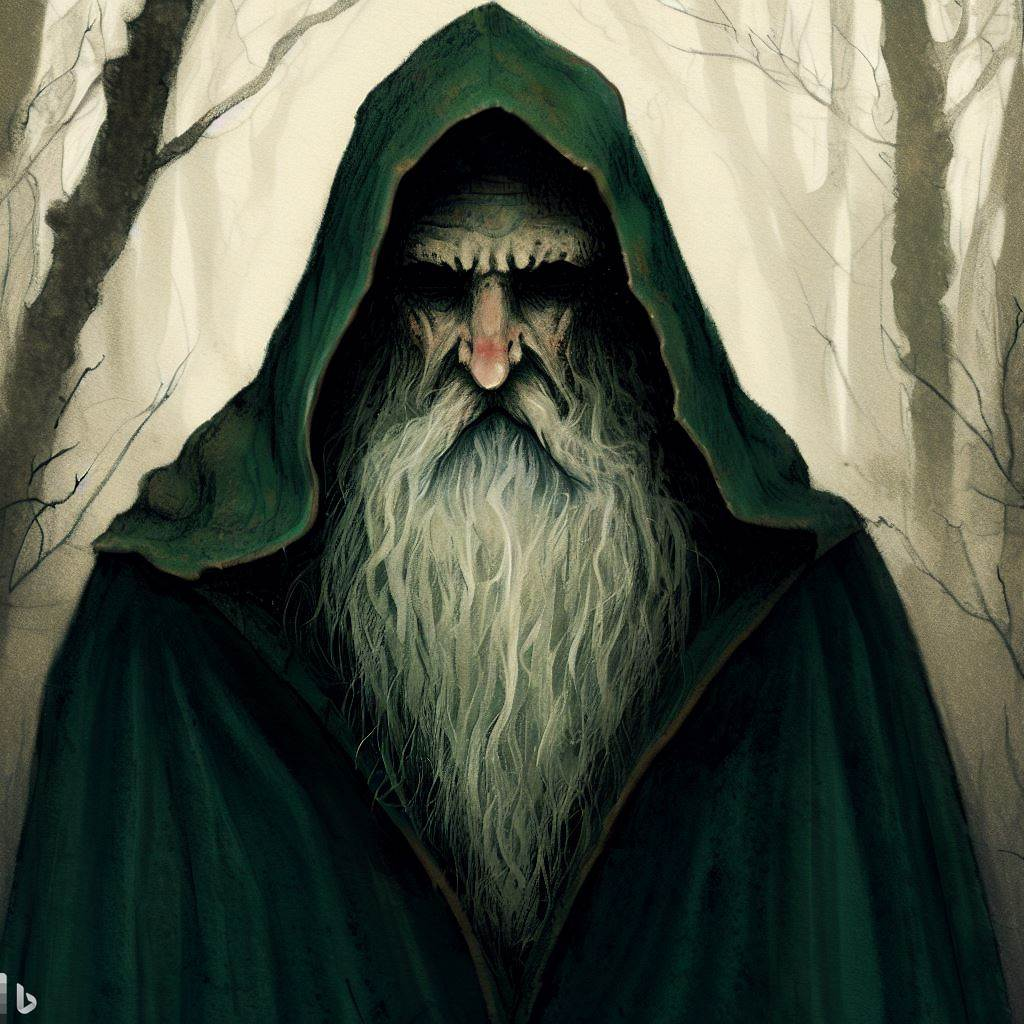
\includegraphics[width=0.99\linewidth]{gmann3.jpeg}
    %\caption{Etherus Schüler}
  \end{subfigure}
\end{figure}

\newpage

\subsection{Wald der Giganten}
\label{sec:org380b861}
\subsubsection{Einhorn\label{einhorn}}
\label{sec:org0d53e5d}
Es ist das letzte seiner Art; sein Blut besitzt enorme Heilkräfte und kann sogar Tote wiederbeleben, weshalb es sehr beliebt ist; Gerüchte gehen in ganz Sommerset umher, dass es noch ein Exemplar gäbe, gesehen hat man es aber noch nicht;
\begin{figure}[H]
\centering
\caption{Das letzte Einhorn}
\label{fig:unicorn}
  \begin{subfigure}{0.3\textwidth}
    \centering
    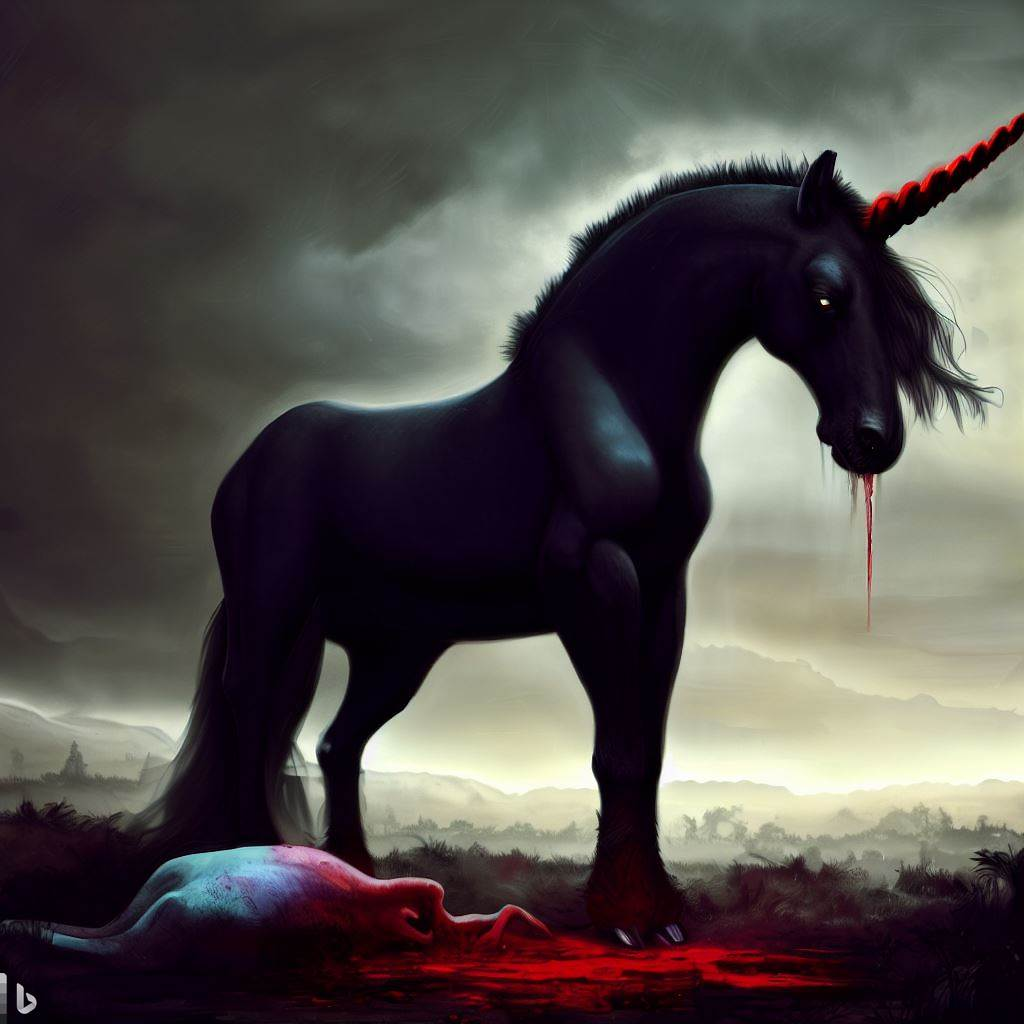
\includegraphics[width=0.99\linewidth]{unicorn1.jpeg}
    \caption{Einhorn nach der Jagd}
  \end{subfigure}%
  \begin{subfigure}{0.3\textwidth}
    \centering
    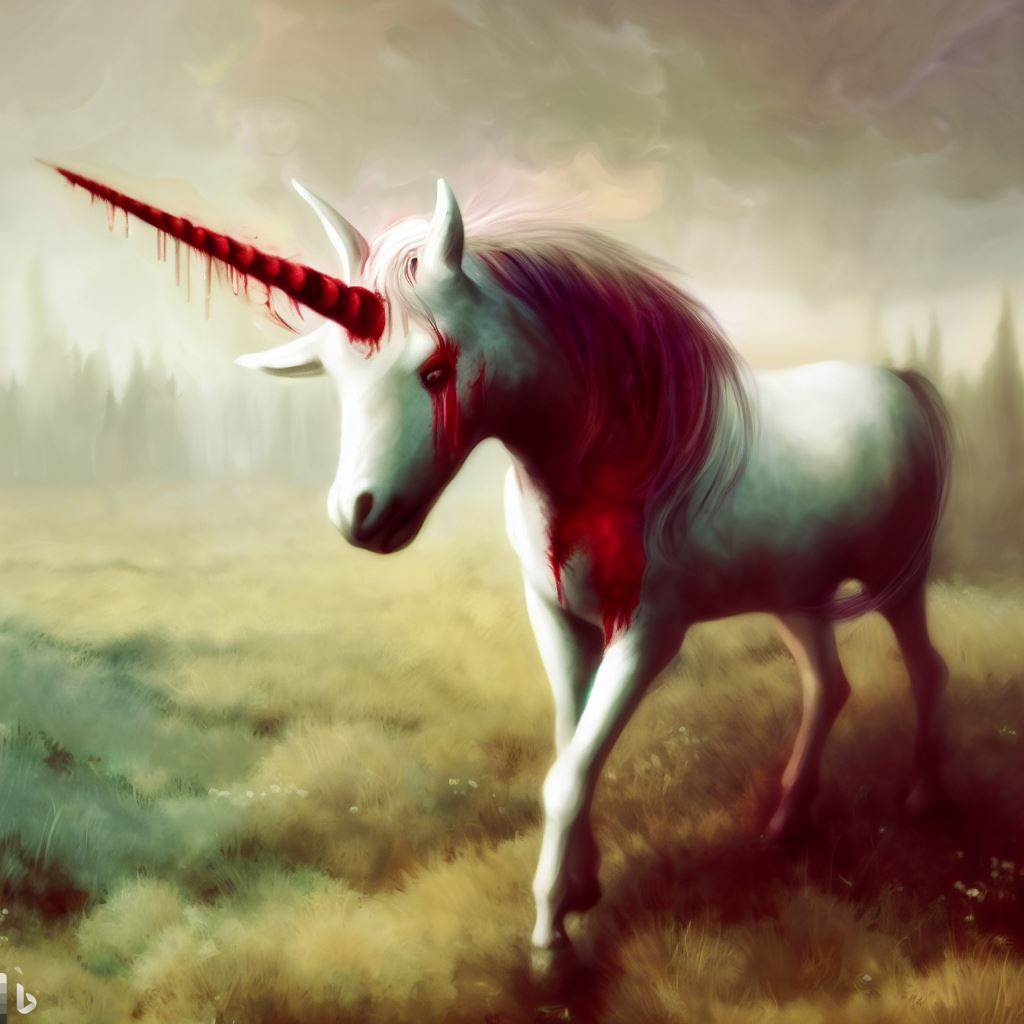
\includegraphics[width=0.99\linewidth]{unicorn2.jpeg}
    \caption{verletztes Einhorn}
  \end{subfigure}%
  \begin{subfigure}{0.3\textwidth}
    \centering
    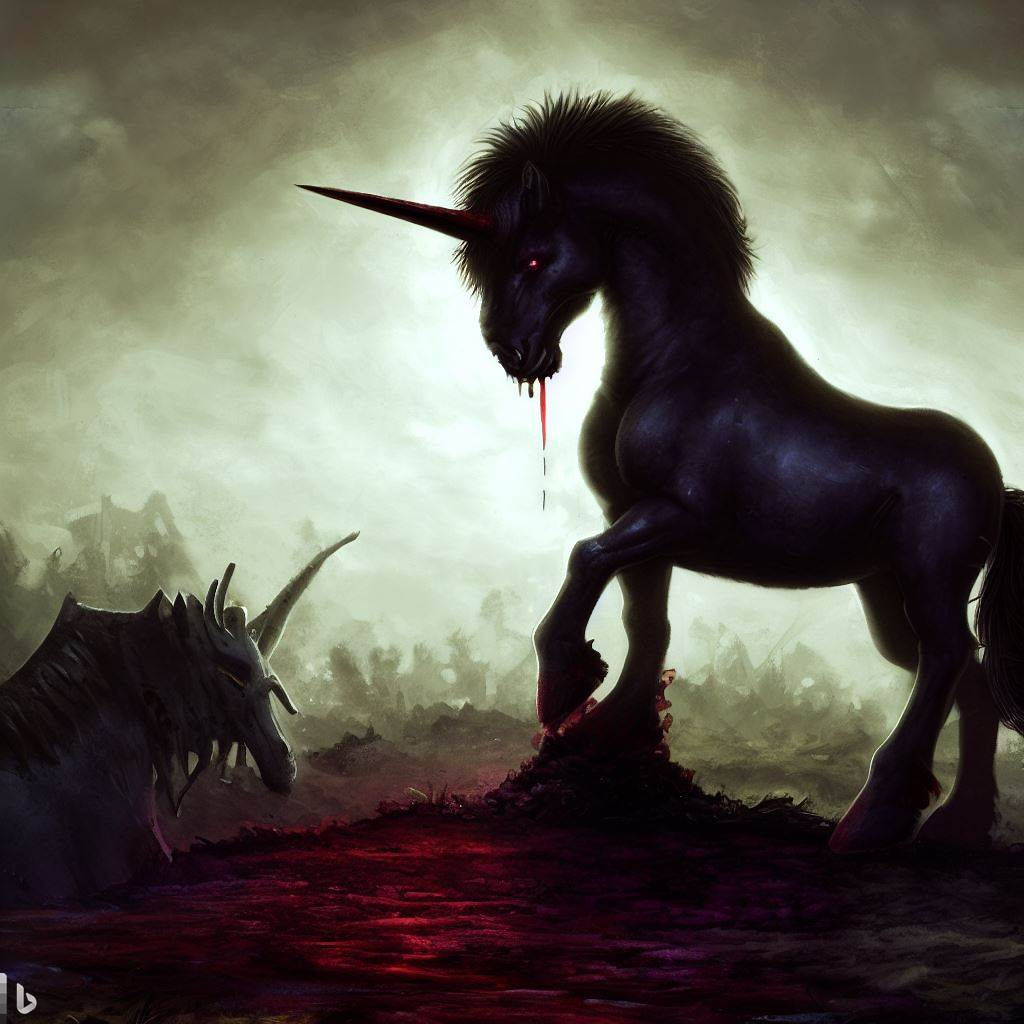
\includegraphics[width=0.99\linewidth]{unicorn3.jpeg}
    \caption{überlebendes Einhorn}
  \end{subfigure}
\end{figure}

\subsubsection{Hippogreif\label{hippo}}
\label{sec:org6b39211}
Mag keine Fremden, lebt alleine, halb Pferd, halb Greif.
\begin{figure}[H]
\centering
\caption{Hippogreif}
\label{fig:hippo}
  \begin{subfigure}{0.3\textwidth}
    \centering
    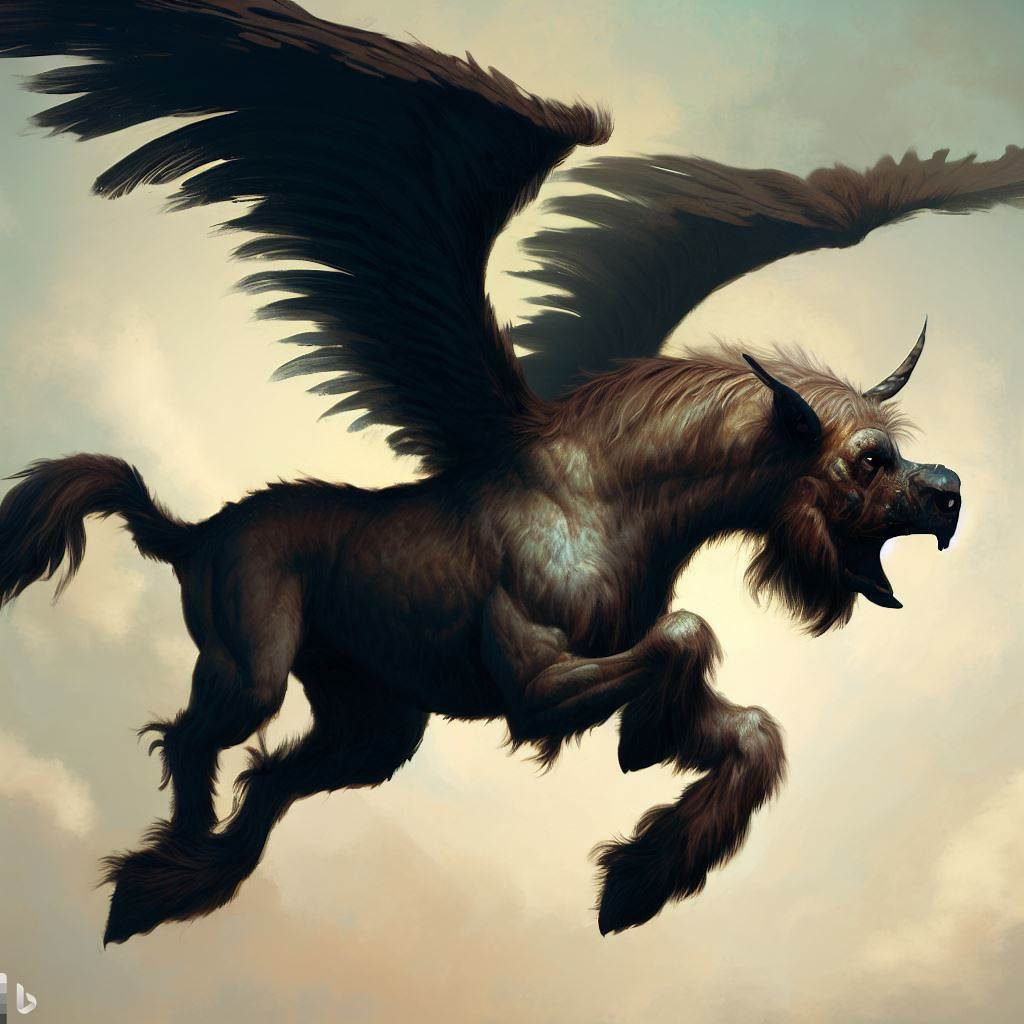
\includegraphics[width=0.99\linewidth]{hippo1.jpeg}
    %\caption{Ethera}
  \end{subfigure}%
  \begin{subfigure}{0.3\textwidth}
    \centering
    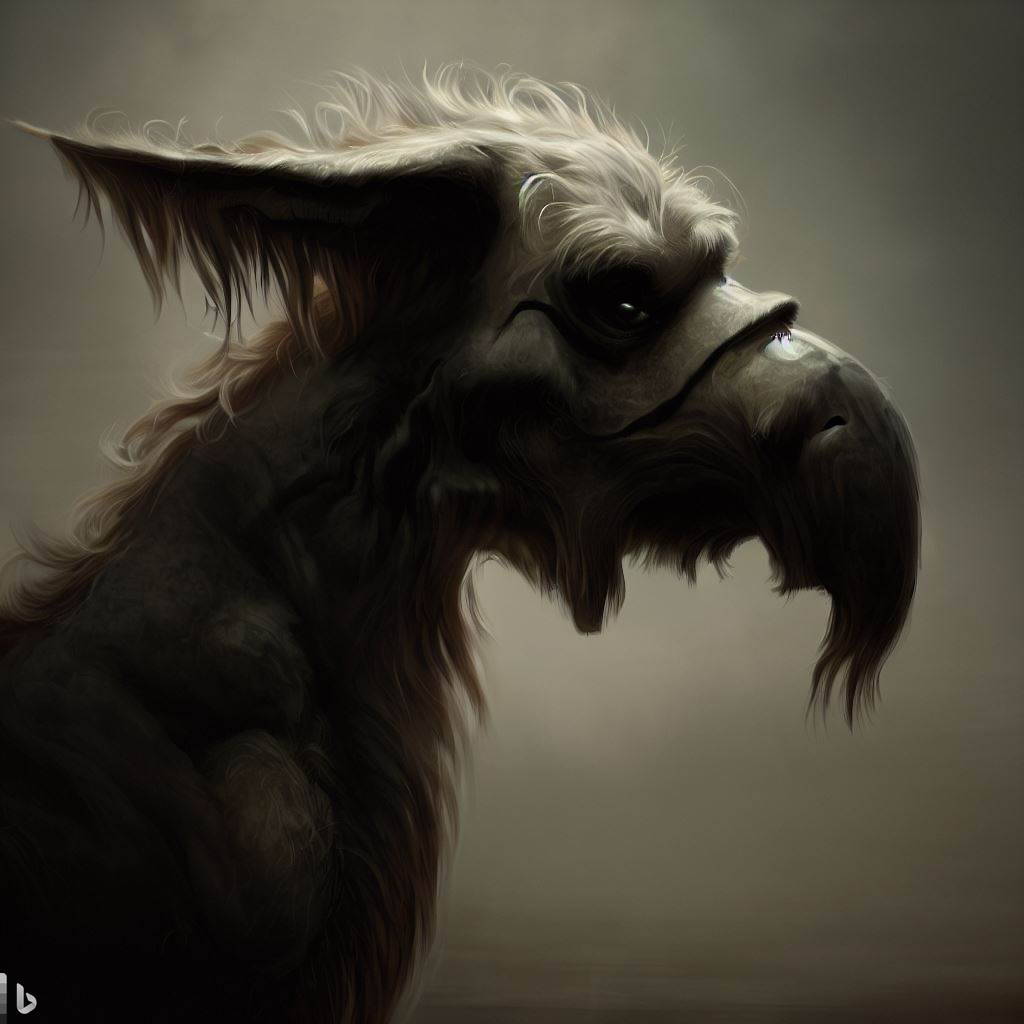
\includegraphics[width=0.99\linewidth]{hippo2.jpeg}
    %\caption{Etherus Meister}
  \end{subfigure}%
  \begin{subfigure}{0.3\textwidth}
    \centering
    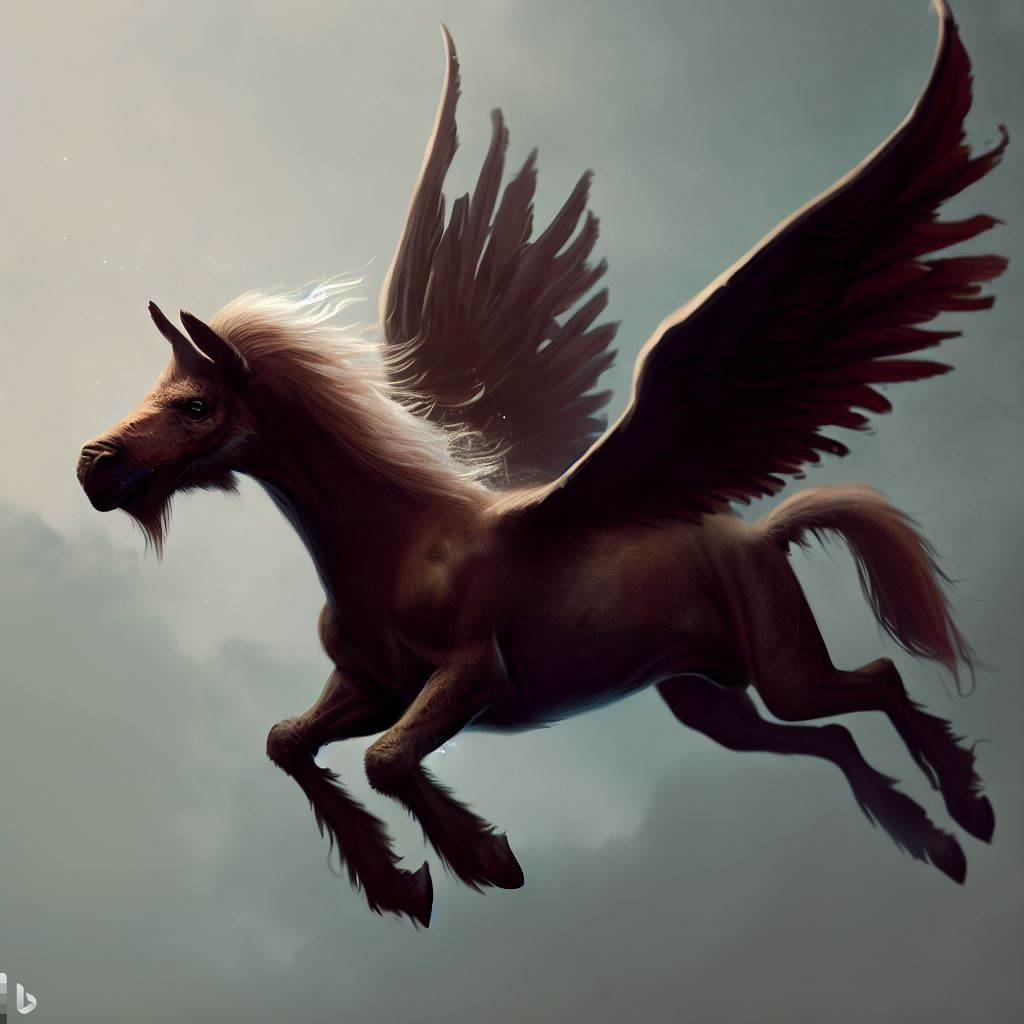
\includegraphics[width=0.99\linewidth]{hippo3.jpeg}
    %\caption{Etherus Schüler}
  \end{subfigure}
\end{figure}

\subsubsection{Golem\label{golem}}
\label{sec:org4941a9b}
Golems sind Lebewesen aus Lehm; niemand weiß, wer sie erschaffen hat; sie sind sehr dumm und langsam; wenn sie treffen, machen sie großen Schaden; sie sehen aus wie Menschen; auf der Stirn klebt ein Zettel mit der Inschrift “emeth” (= Leben); gelingt es den Abenteurern, den Zettel zu zerstören oder herunterzureißen oder gar in Brand zusetzen, zerfällt er wieder zu Lehm;
\begin{figure}[H]
\centering
\caption{Golem}
\label{fig:golem}
  \begin{subfigure}{0.3\textwidth}
    \centering
    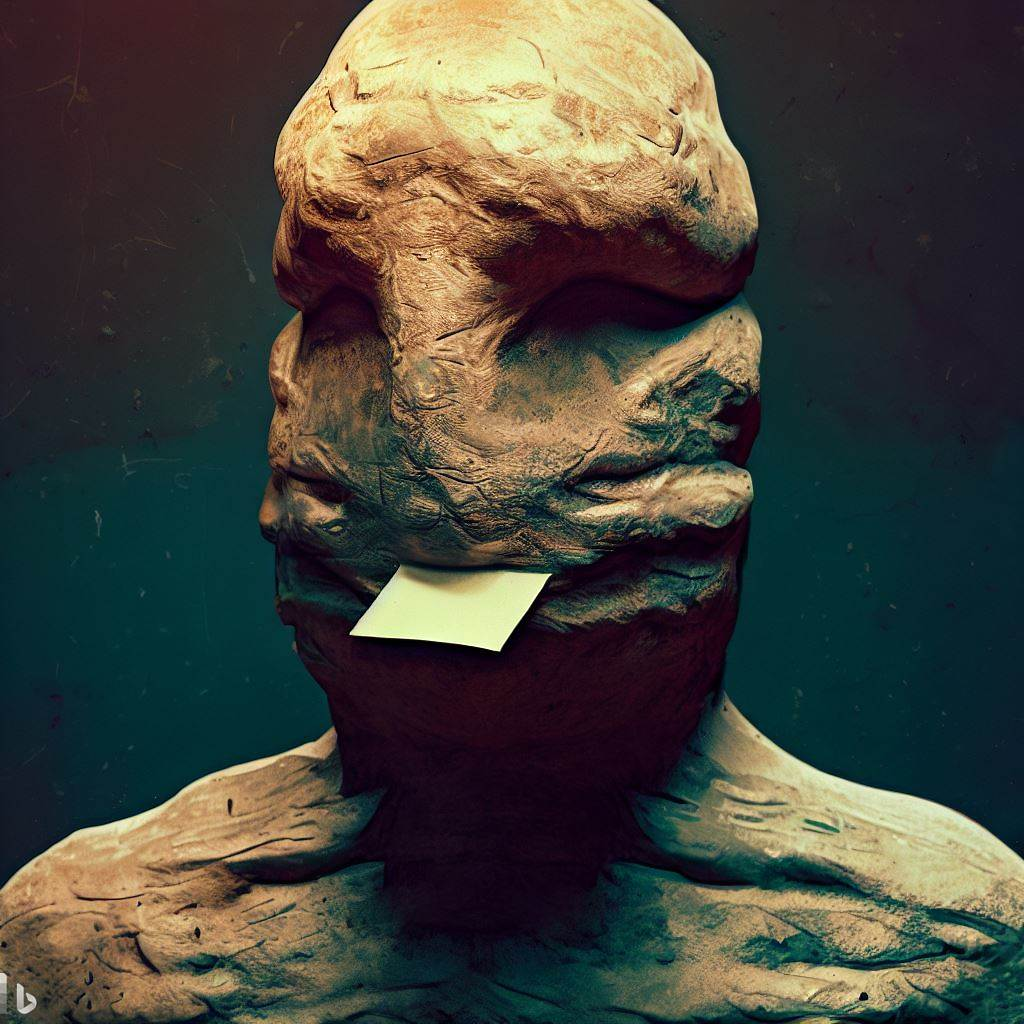
\includegraphics[width=0.99\linewidth]{golem1.jpeg}
    %\caption{Ethera}
  \end{subfigure}%
  \begin{subfigure}{0.3\textwidth}
    \centering
    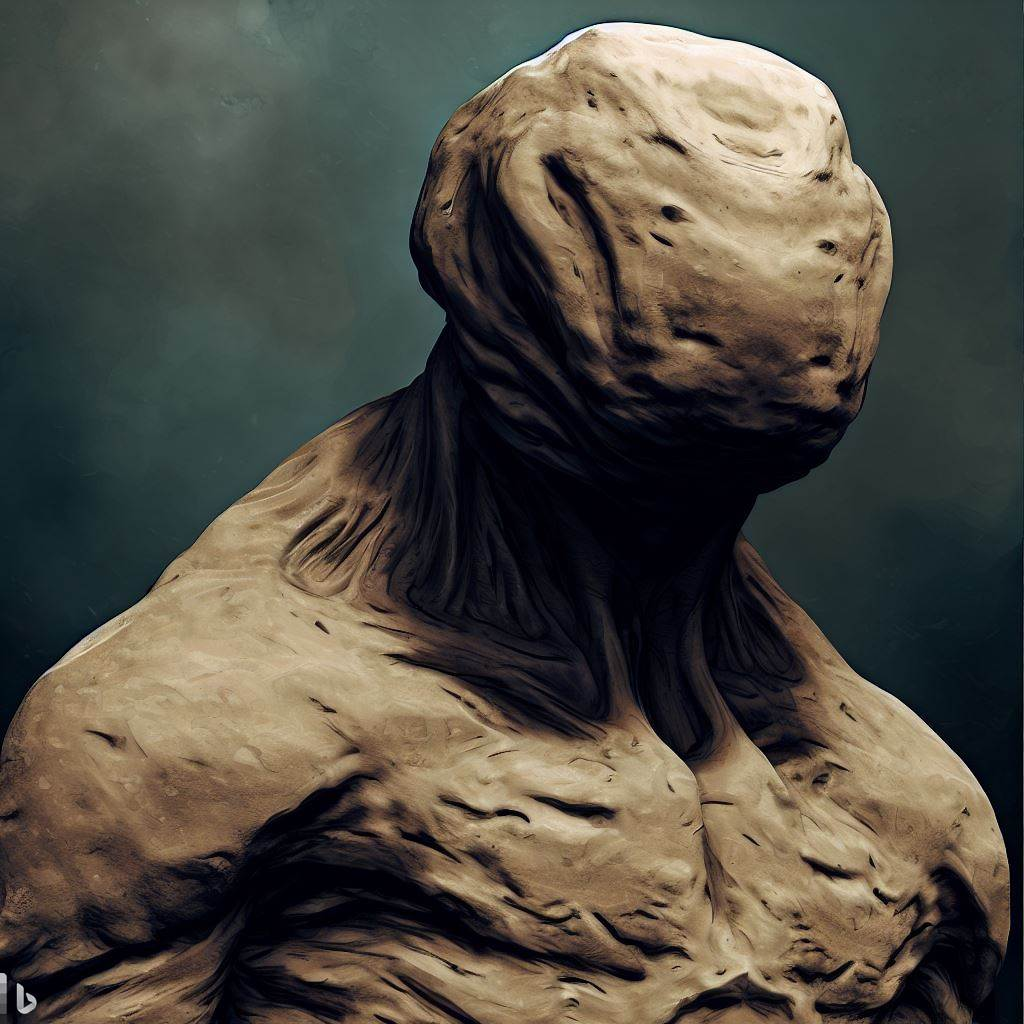
\includegraphics[width=0.99\linewidth]{golem2.jpeg}
    %\caption{Etherus Meister}
  \end{subfigure}%
  \begin{subfigure}{0.3\textwidth}
    \centering
    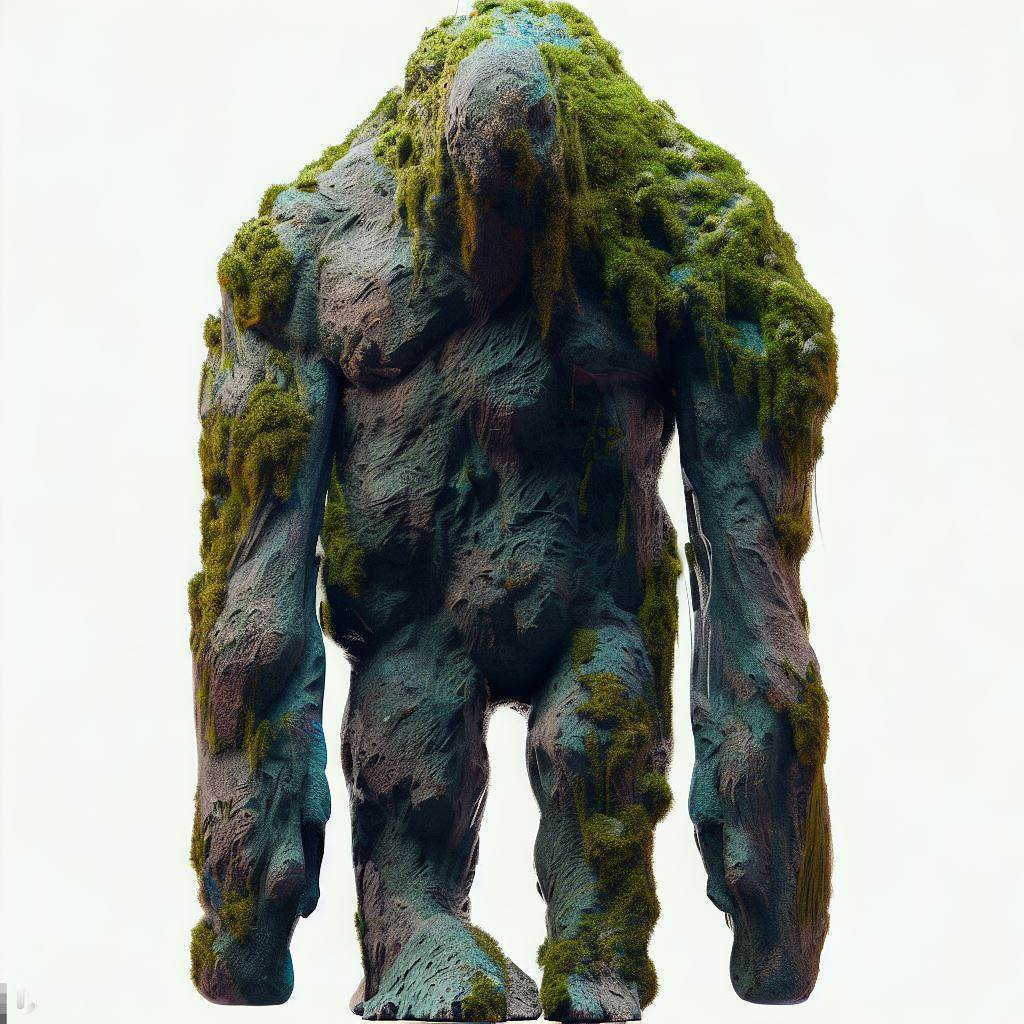
\includegraphics[width=0.99\linewidth]{golem3.jpeg}
    %\caption{Etherus Schüler}
  \end{subfigure}
\end{figure}

\newpage

\subsection{Totmannsruh}
\label{sec:org5d865b5}
\subsubsection{Yeti\label{yeti}}
\label{sec:org639fd13}
Affenmenschliches, scheues, aber dennoch aggressives Wesen; wurde seit jeher von Menschen gejagt und verabscheut diese Rasse, ist jedoch anderen Lebewesen gegenüber neutral gesinnt; ist sehr stark und hat eine große Ausdauer, kämpft mit einem riesigen Holzstock
\begin{figure}[H]
\centering
\caption{Yeti}
\label{fig:yeti}
  \begin{subfigure}{0.3\textwidth}
    \centering
    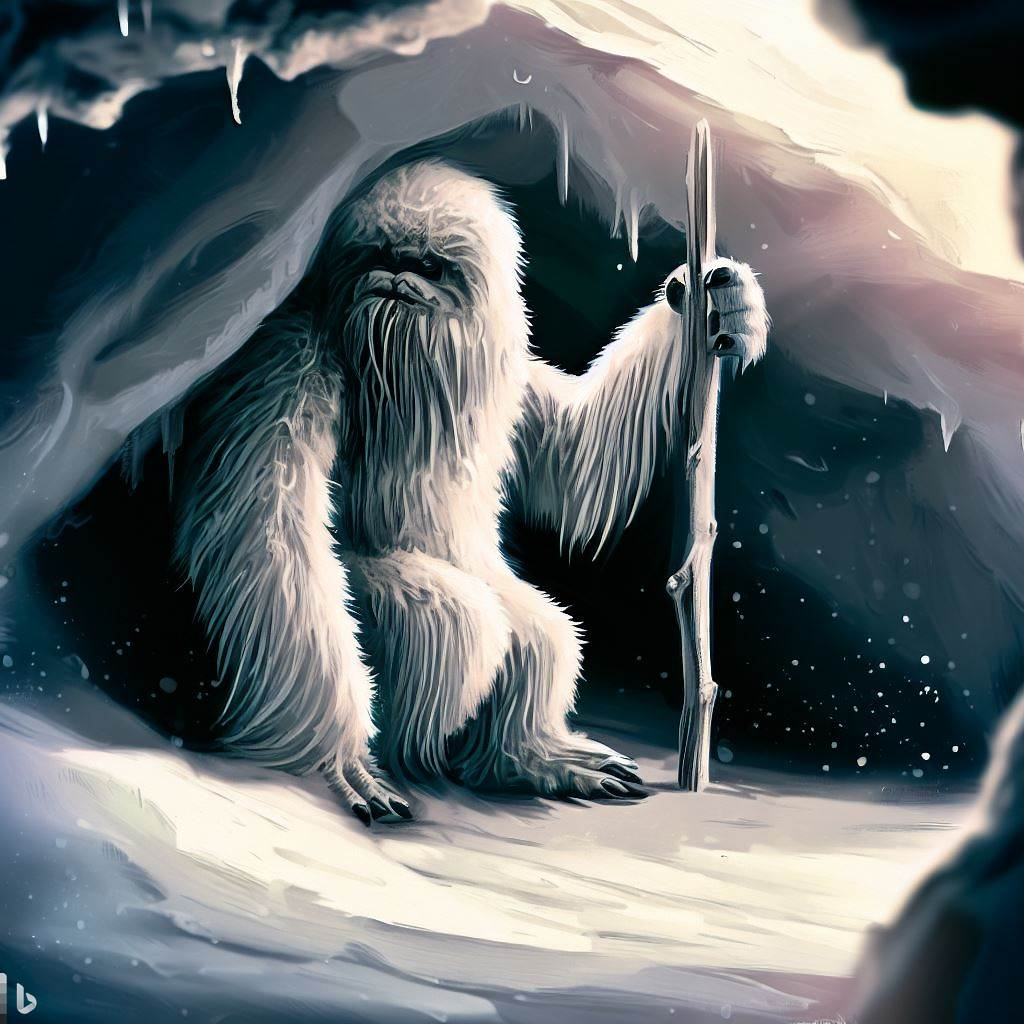
\includegraphics[width=0.99\linewidth]{yeti1.jpeg}
    %\caption{Ethera}
  \end{subfigure}%
  \begin{subfigure}{0.3\textwidth}
    \centering
    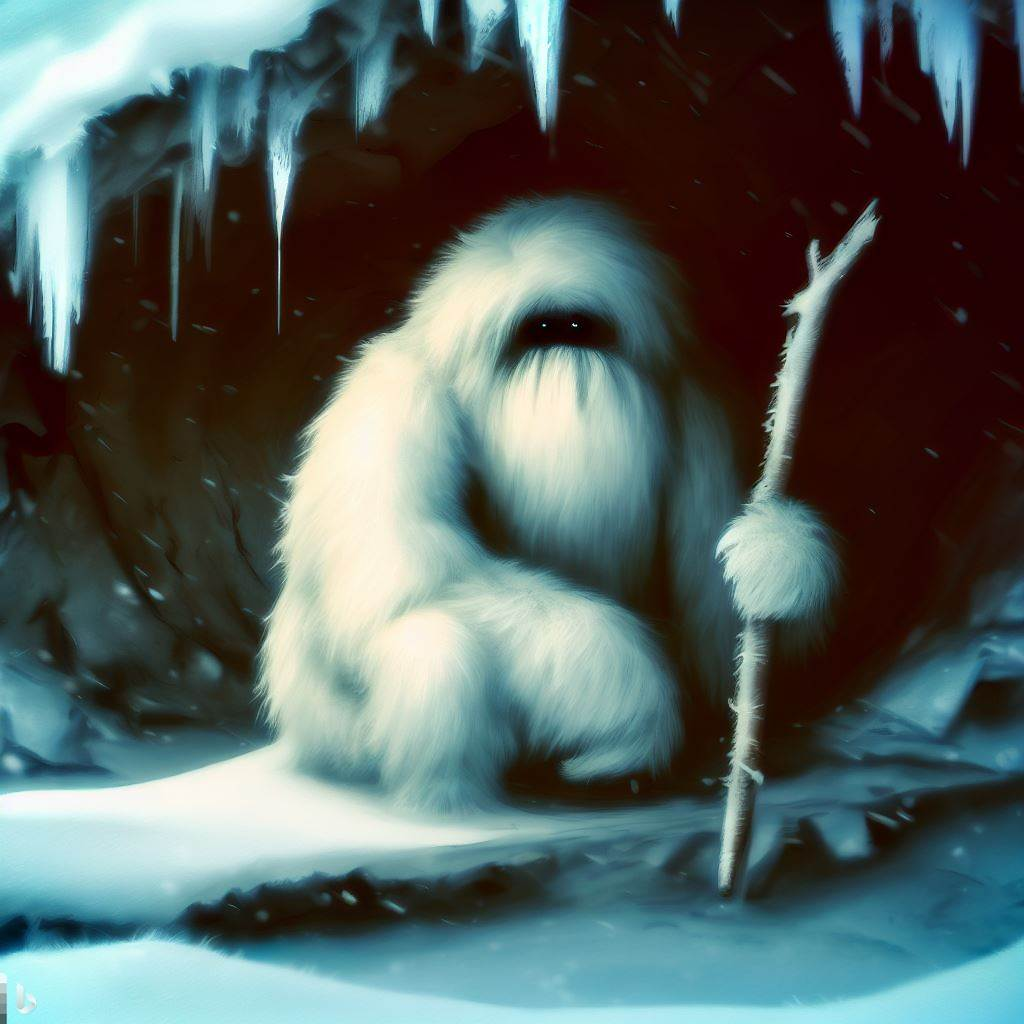
\includegraphics[width=0.99\linewidth]{yeti2.jpeg}
    %\caption{Etherus Meister}
  \end{subfigure}%
  \begin{subfigure}{0.3\textwidth}
    \centering
    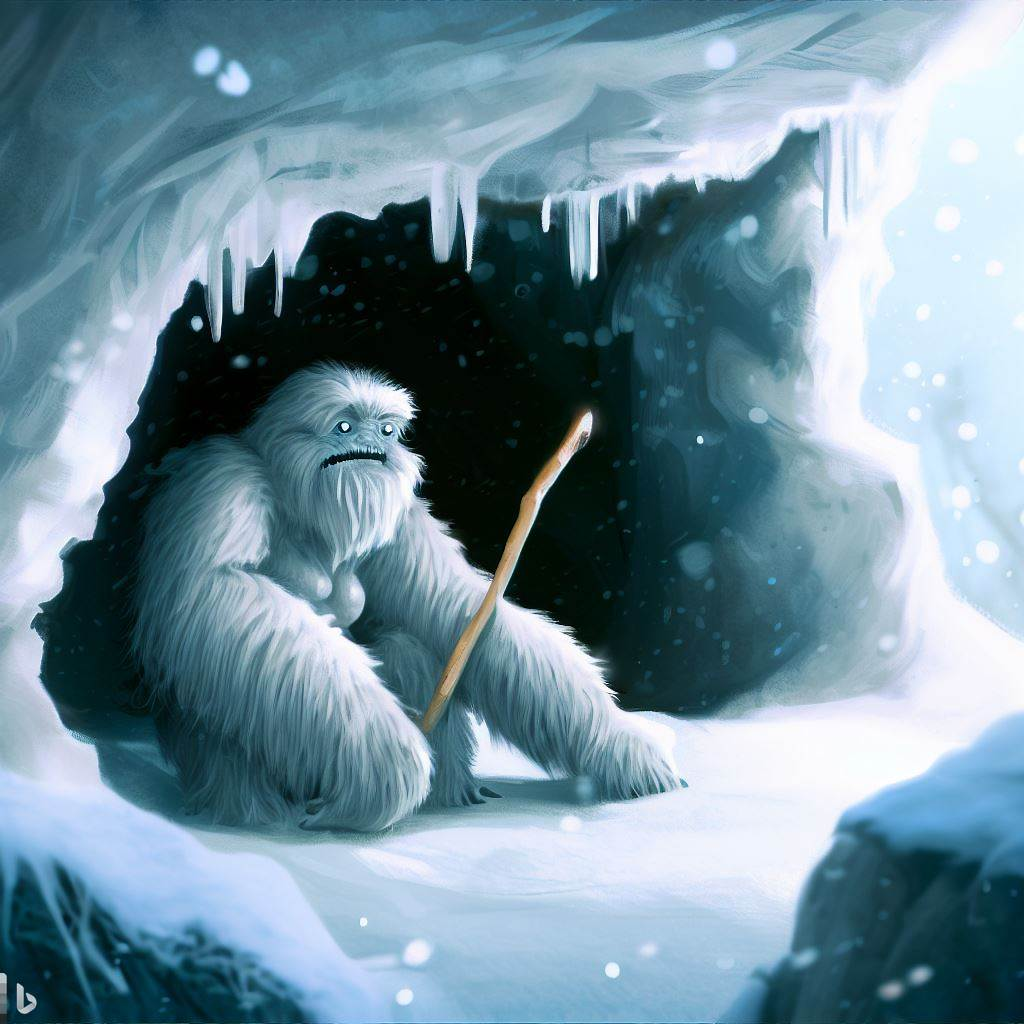
\includegraphics[width=0.99\linewidth]{yeti3.jpeg}
    %\caption{Etherus Schüler}
  \end{subfigure}
\end{figure}

\subsubsection{Zerberus\label{zerberus}}
\label{sec:orga8af7d3}
2 Meter großer Wolf mit 3 Köpfen und riesigen Fangzähnen; ist ein Bruder der einköpfigen Chimäre und höchst gefährlich; hat einen hohen Verteidigungswert und ist sehr stark
\begin{figure}[H]
\centering
\caption{Zerberus}
\label{fig:dogo}
  \begin{subfigure}{0.3\textwidth}
    \centering
    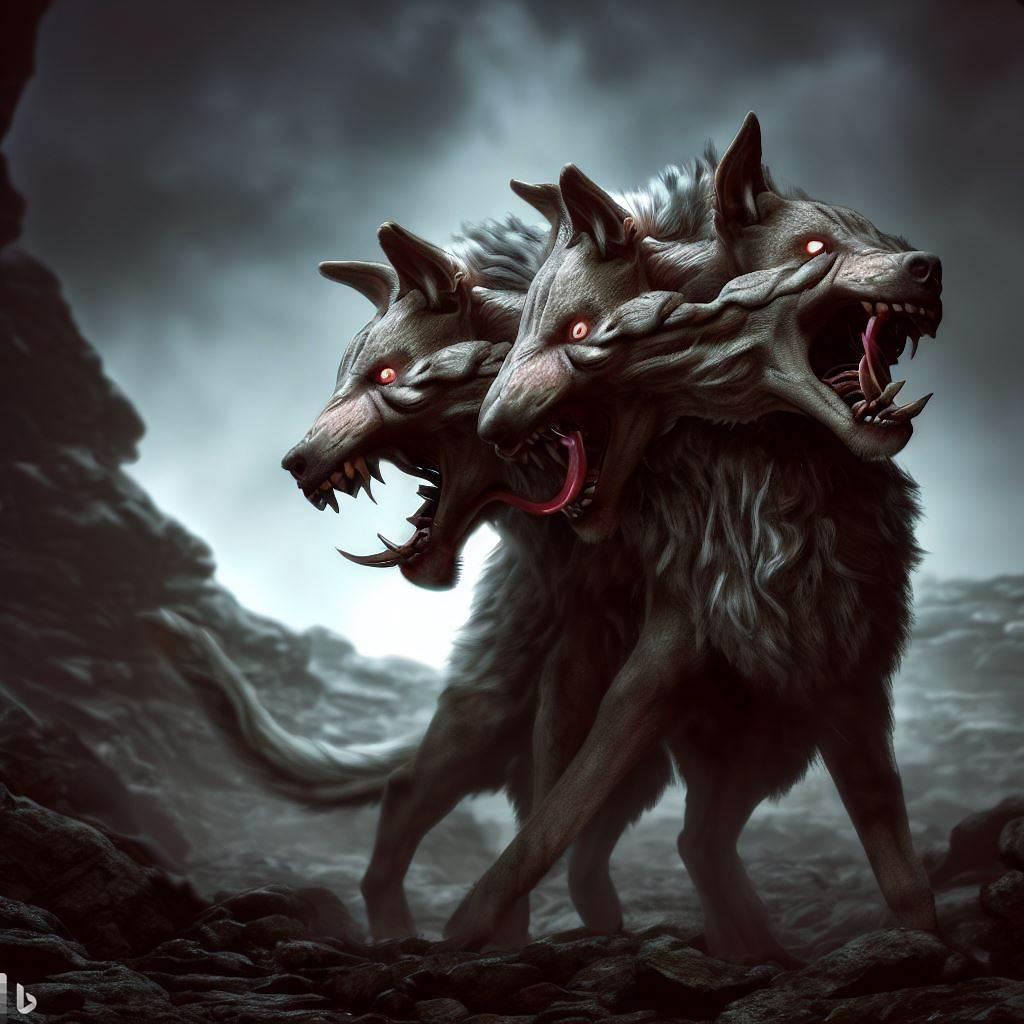
\includegraphics[width=0.99\linewidth]{dogo1.jpeg}
    %\caption{Ethera}
  \end{subfigure}%
  \begin{subfigure}{0.3\textwidth}
    \centering
    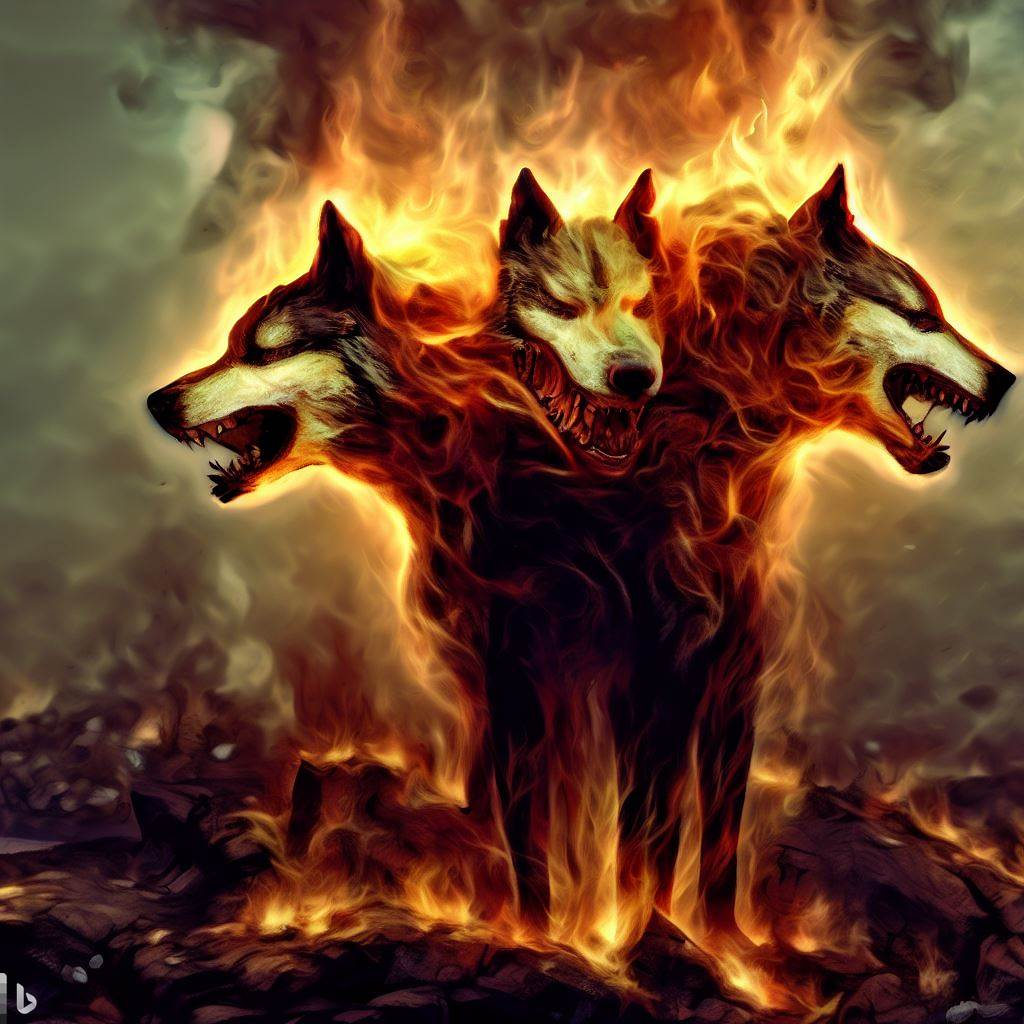
\includegraphics[width=0.99\linewidth]{dogo2.jpeg}
    %\caption{Etherus Meister}
  \end{subfigure}%
  \begin{subfigure}{0.3\textwidth}
    \centering
    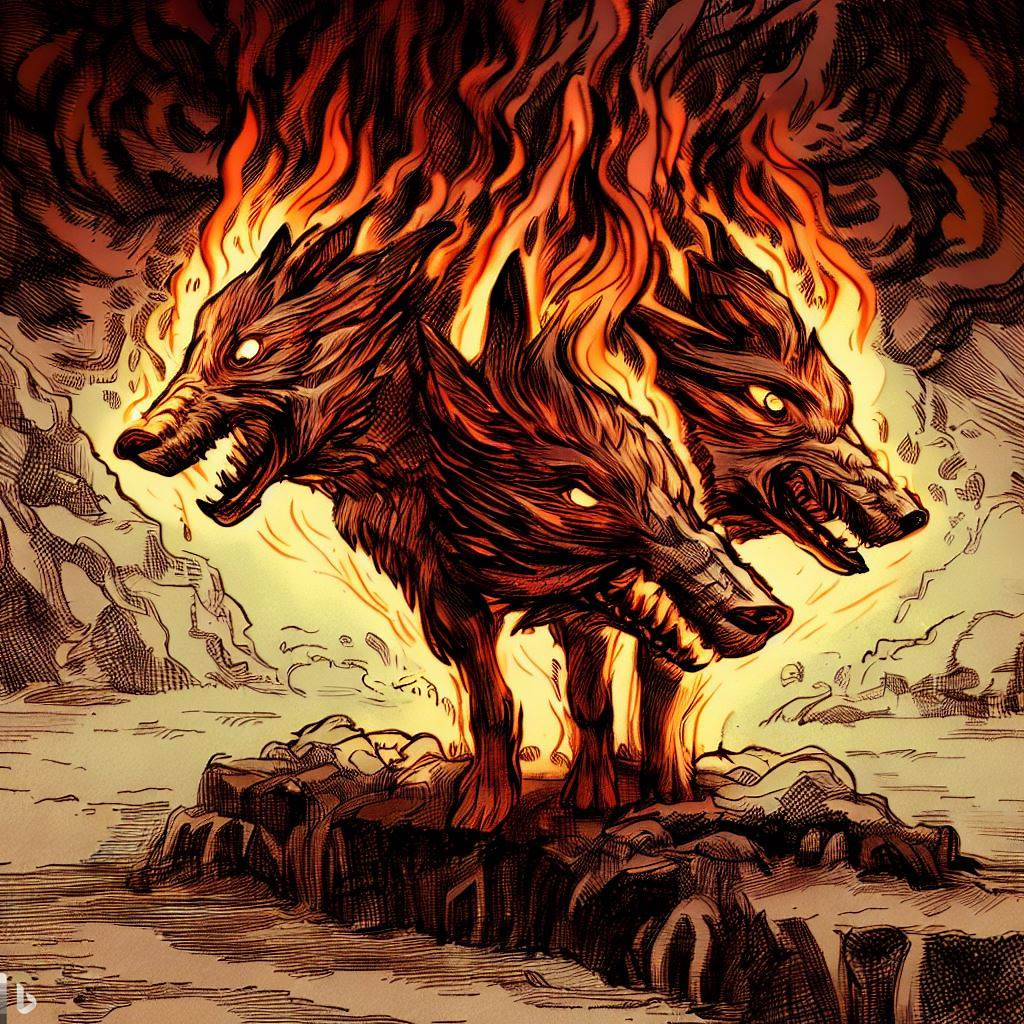
\includegraphics[width=0.99\linewidth]{dogo3.jpeg}
    %\caption{Etherus Schüler}
  \end{subfigure}
\end{figure}

\subsubsection{Werwölfe\label{werwolf}}
\label{sec:orga0bb00a}
unterstehen Zerberus und sind sehr aggressiv und gefährlich; sie riechen außerordentlich gut und fressen alles, was ihnen in die Quere kommt; untertags stellen sie ein menschliches Bergvolk dar, während sie in der Nacht zu blutrünstigen Monstern werden;
\begin{figure}[H]
\centering
\caption{Werwolf}
\label{fig:wolf}
  \begin{subfigure}{0.3\textwidth}
    \centering
    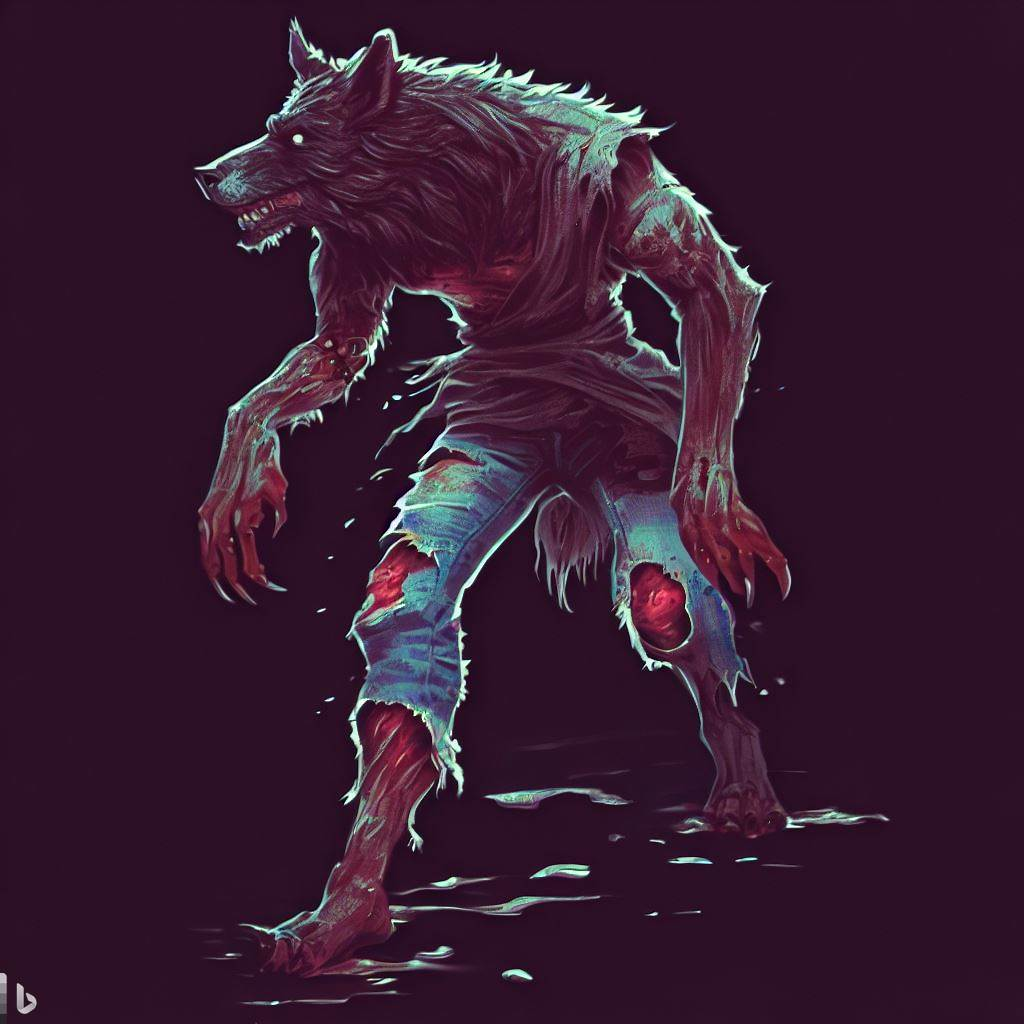
\includegraphics[width=0.99\linewidth]{wolf1.jpeg}
    %\caption{Ethera}
  \end{subfigure}%
  \begin{subfigure}{0.3\textwidth}
    \centering
    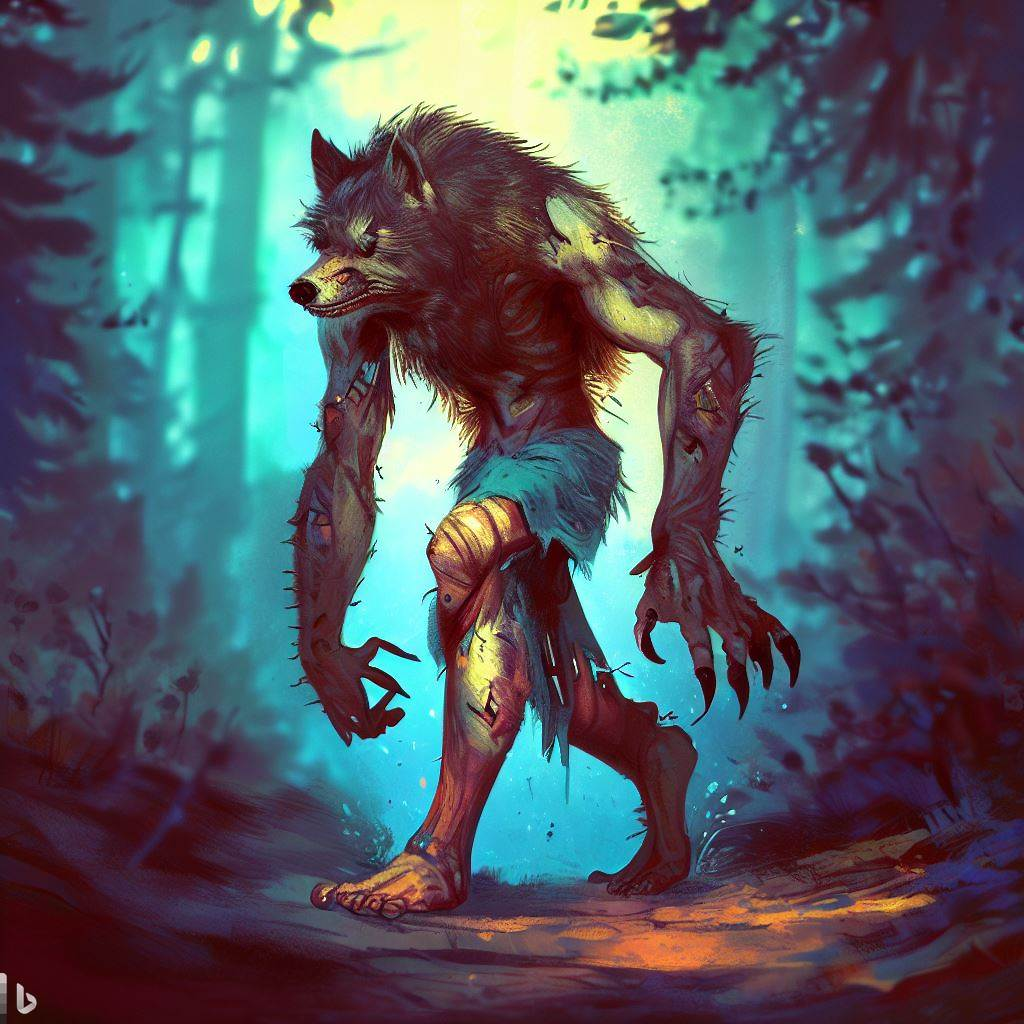
\includegraphics[width=0.99\linewidth]{wolf2.jpeg}
    %\caption{Etherus Meister}
  \end{subfigure}%
  \begin{subfigure}{0.3\textwidth}
    \centering
    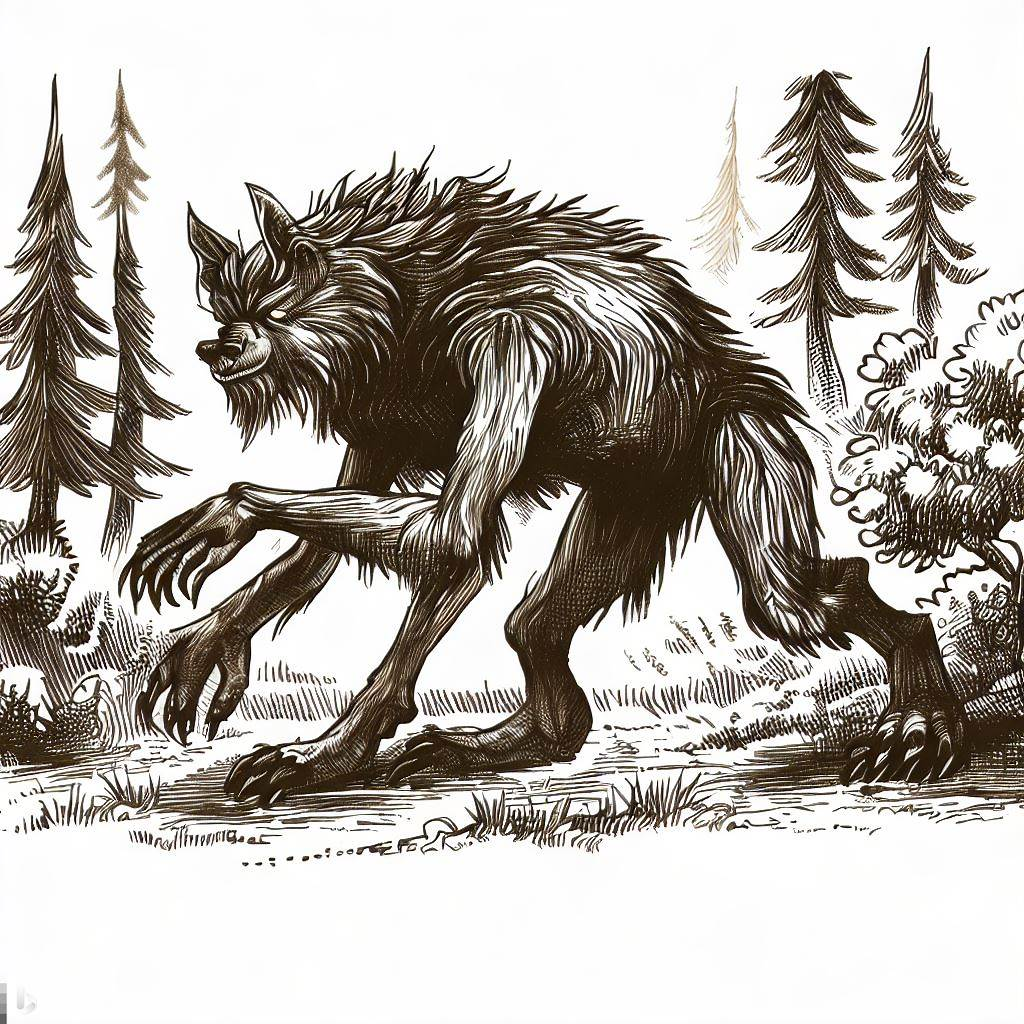
\includegraphics[width=0.99\linewidth]{wolf3.jpeg}
    %\caption{Etherus Schüler}
  \end{subfigure}
\end{figure}

\newpage

\subsection{Astrario}
\label{sec:orgd2418e1}
\subsubsection{Etherus (pl. Etheri)\label{etheri}}
\label{sec:org03b97bd}
Menschliche Zaubergelehrte die als Quelle ihrer Kraft die Leere anzapfen müssen. Die meisten Etheri wissen nichts von der Leere und glauben ihre Kraft kommt von einem Amulett das ihre natürlichen Fähigkeiten bündelt.
\begin{figure}[H]
\centering
\caption{Etheri}
\label{fig:etheri}
  \begin{subfigure}{0.3\textwidth}
    \centering
    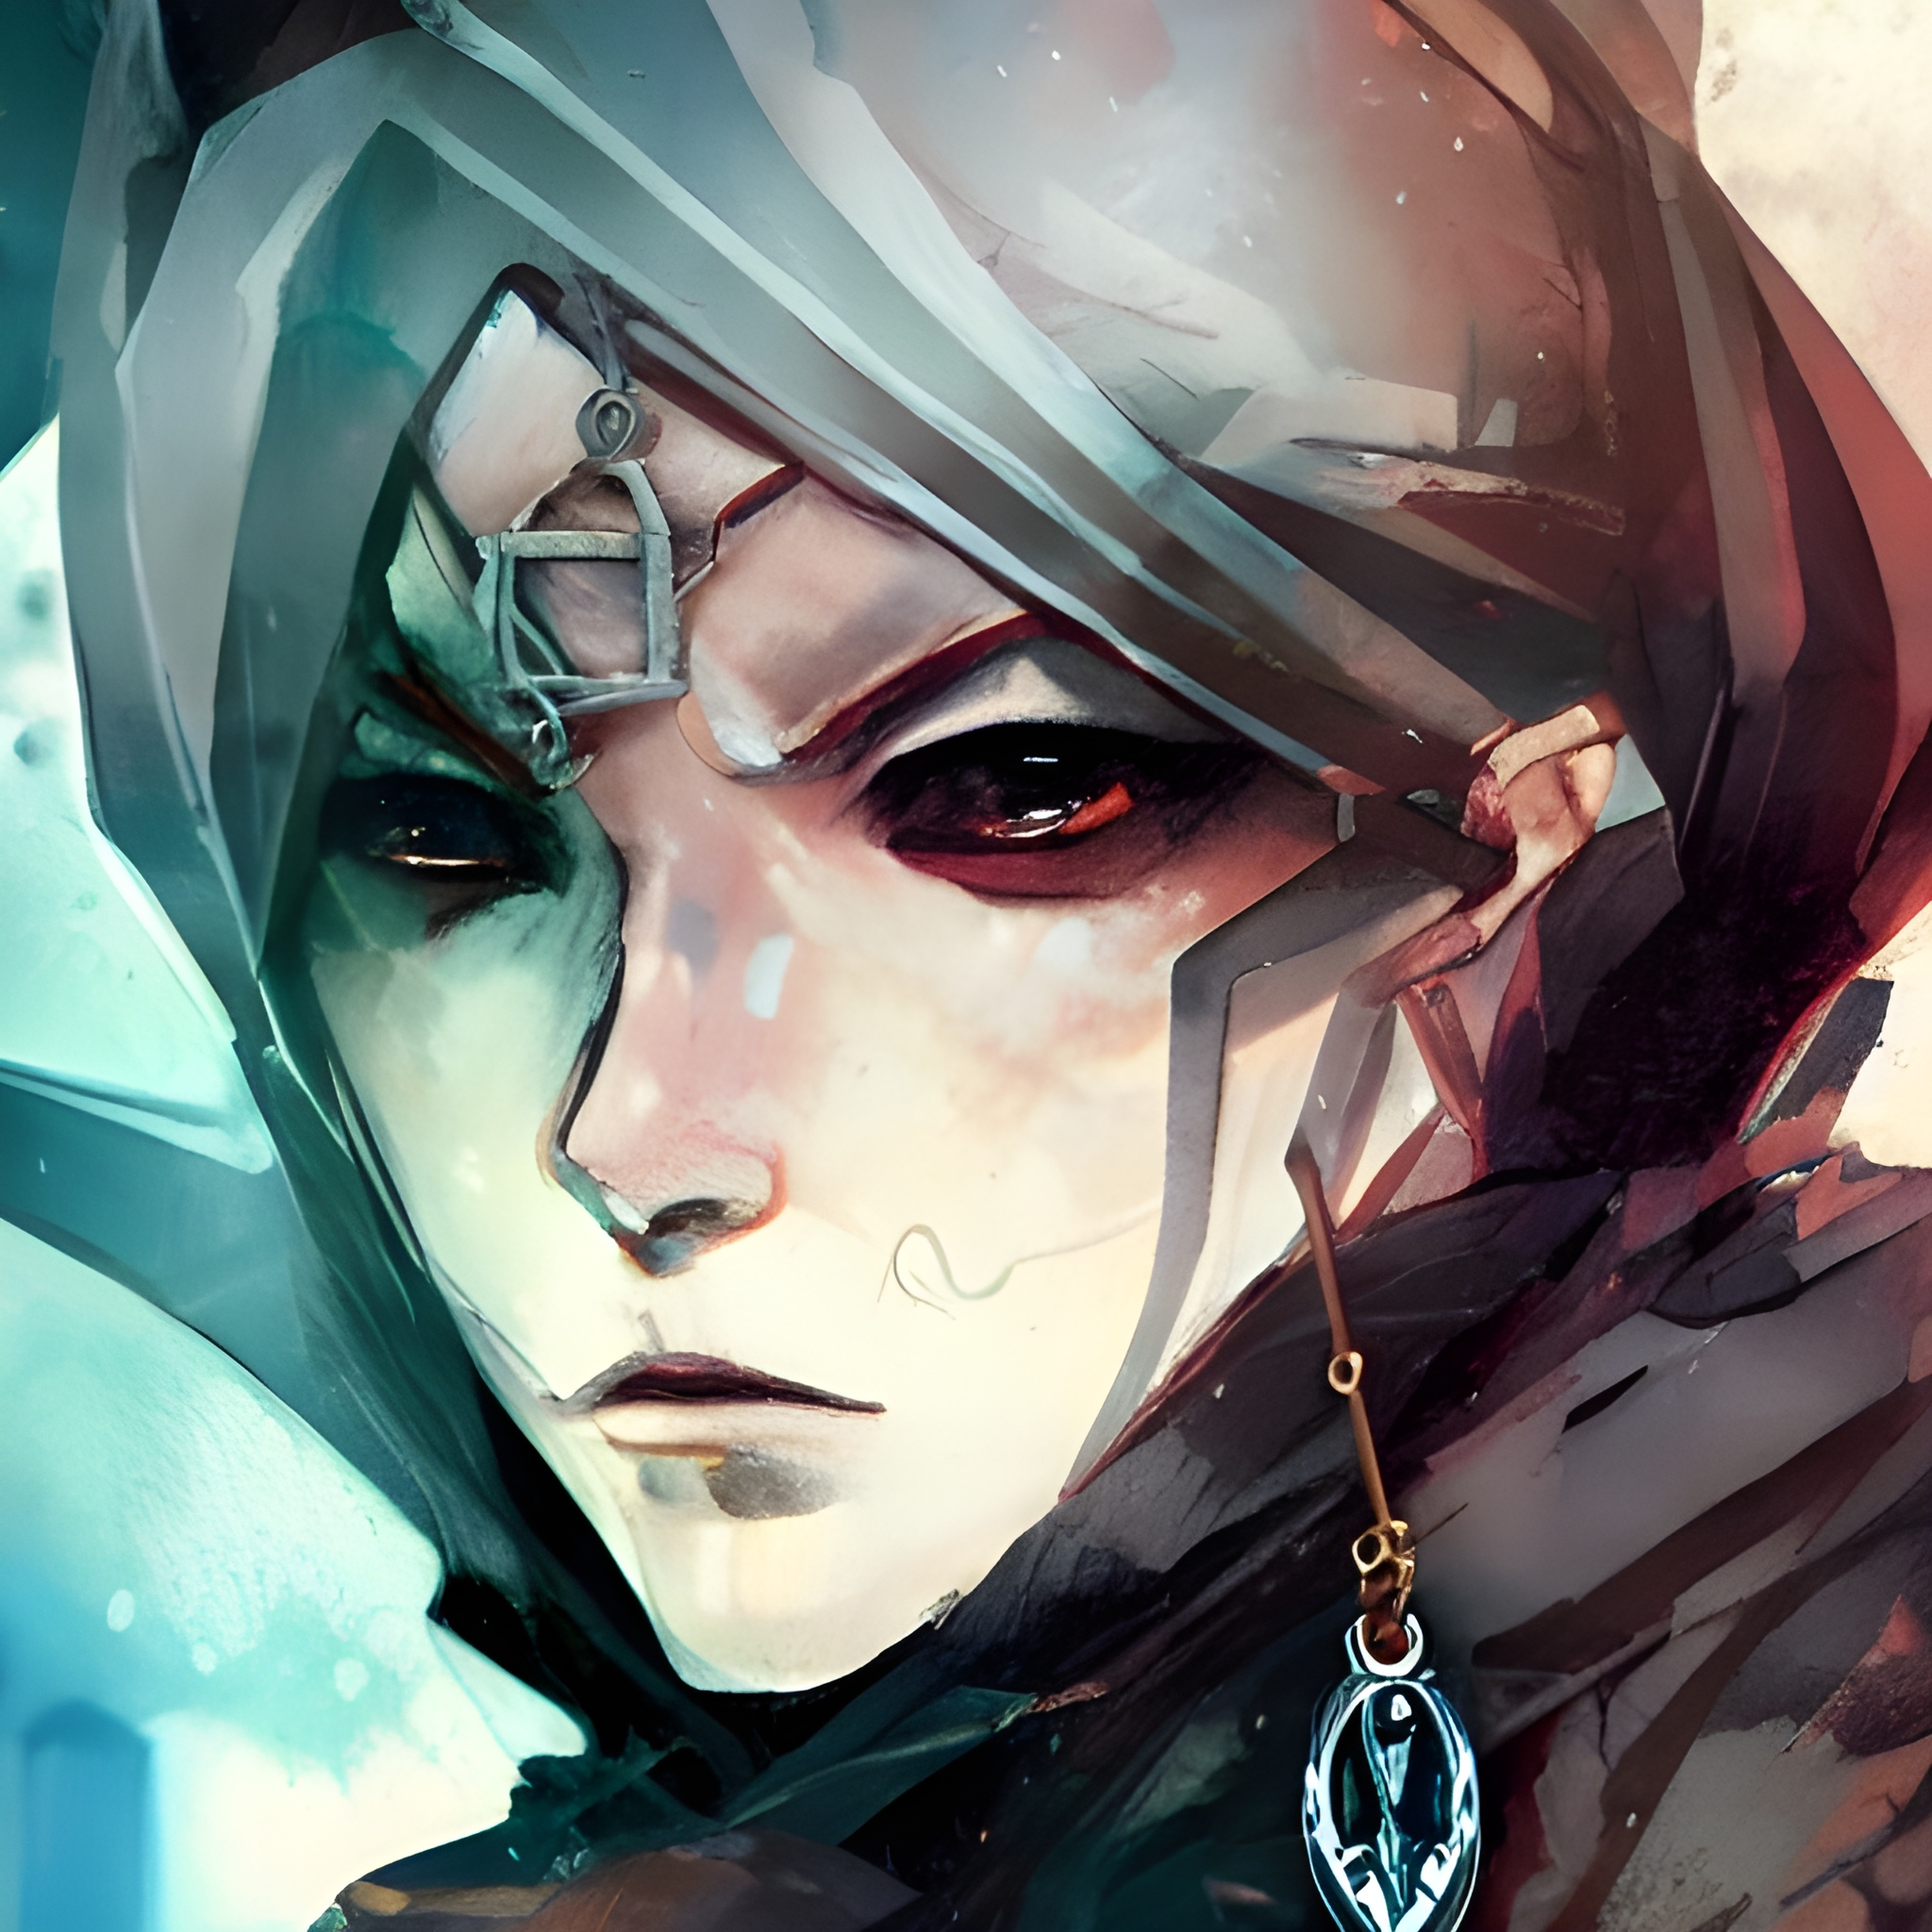
\includegraphics[width=0.99\linewidth]{etheri1.jpeg}
    \caption{Ethera}
  \end{subfigure}%
  \begin{subfigure}{0.3\textwidth}
    \centering
    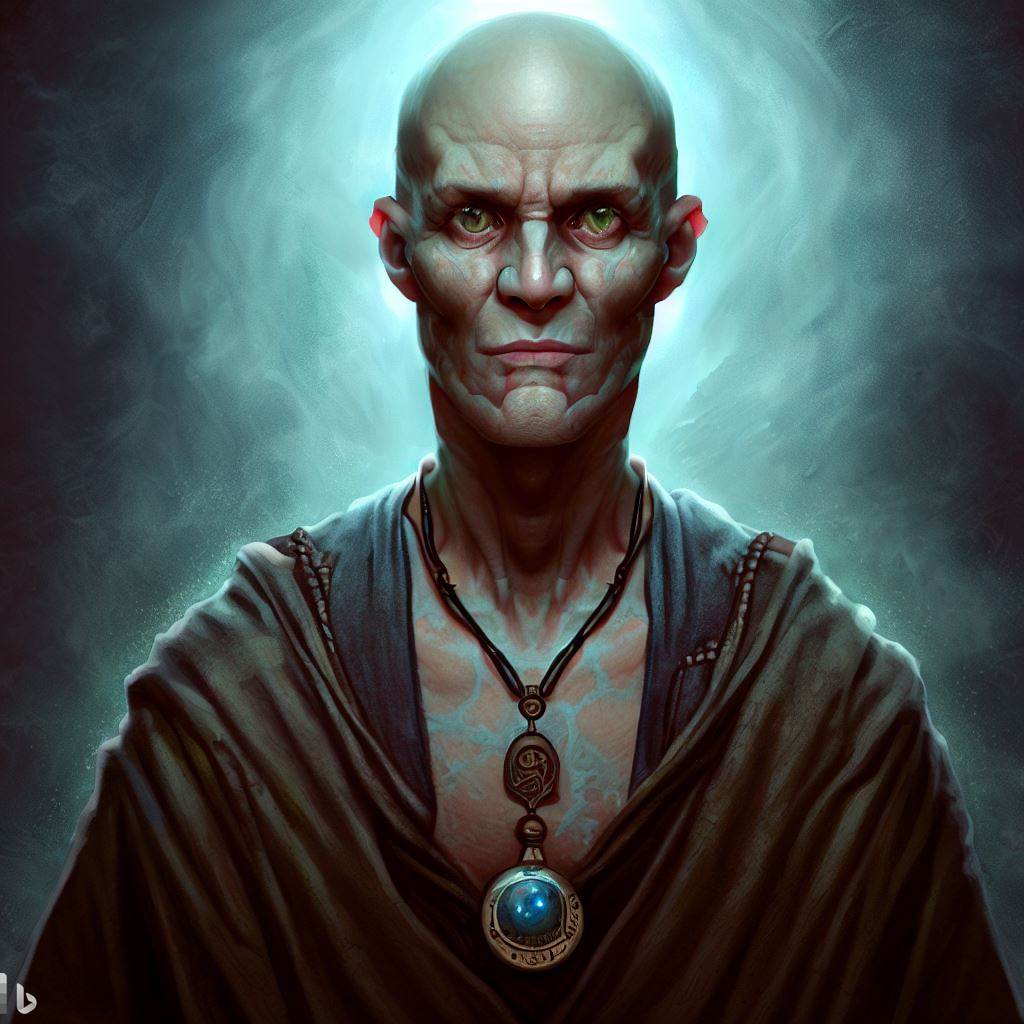
\includegraphics[width=0.99\linewidth]{etheri2.jpeg}
    \caption{Etherus Meister}
  \end{subfigure}%
  \begin{subfigure}{0.3\textwidth}
    \centering
    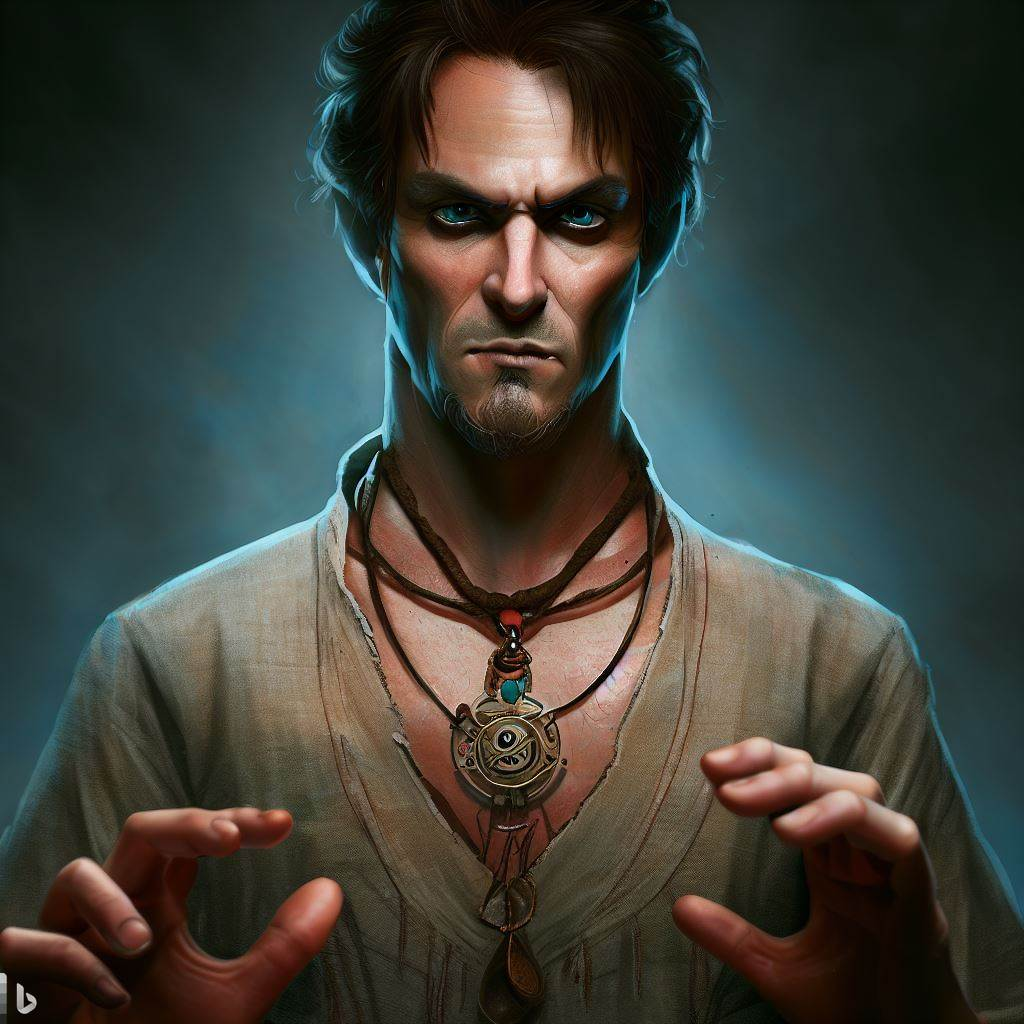
\includegraphics[width=0.99\linewidth]{etheri3.jpeg}
    \caption{Etherus Schüler}
  \end{subfigure}
\end{figure}

\subsubsection{Sphinx\label{sphinx}}
\label{sec:orgd2a8fb5}
Lebt in den Katakomben von Astrario, ist ein uraltes und sehr weises Wesen. Ist den Lebewesen gut gesinnt, verabscheut die schwarzen Bücher.
\begin{figure}[H]
\centering
\caption{Sphinx}
\label{fig:sphinx}
  \begin{subfigure}{0.3\textwidth}
    \centering
    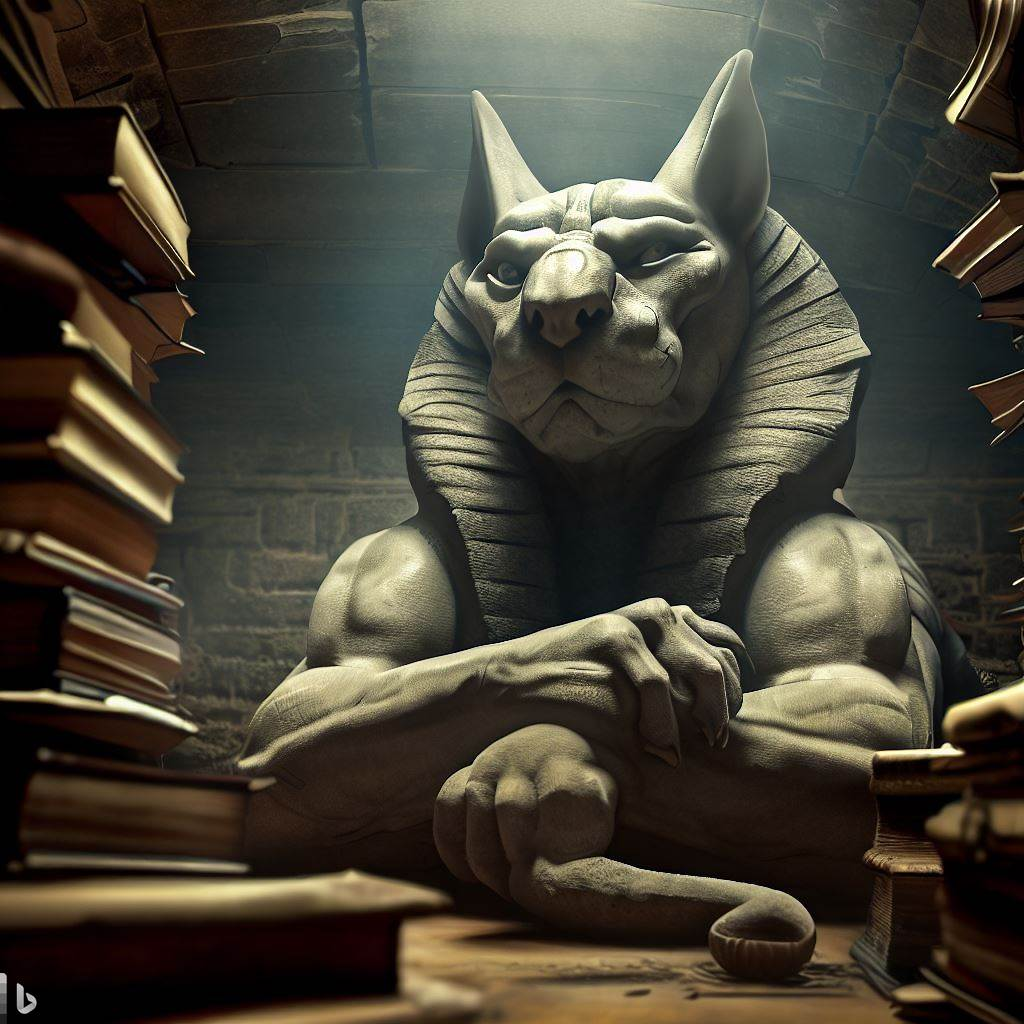
\includegraphics[width=0.99\linewidth]{sphinx1.jpeg}
    \caption{alte Sphinx}
  \end{subfigure}%
  \begin{subfigure}{0.3\textwidth}
    \centering
    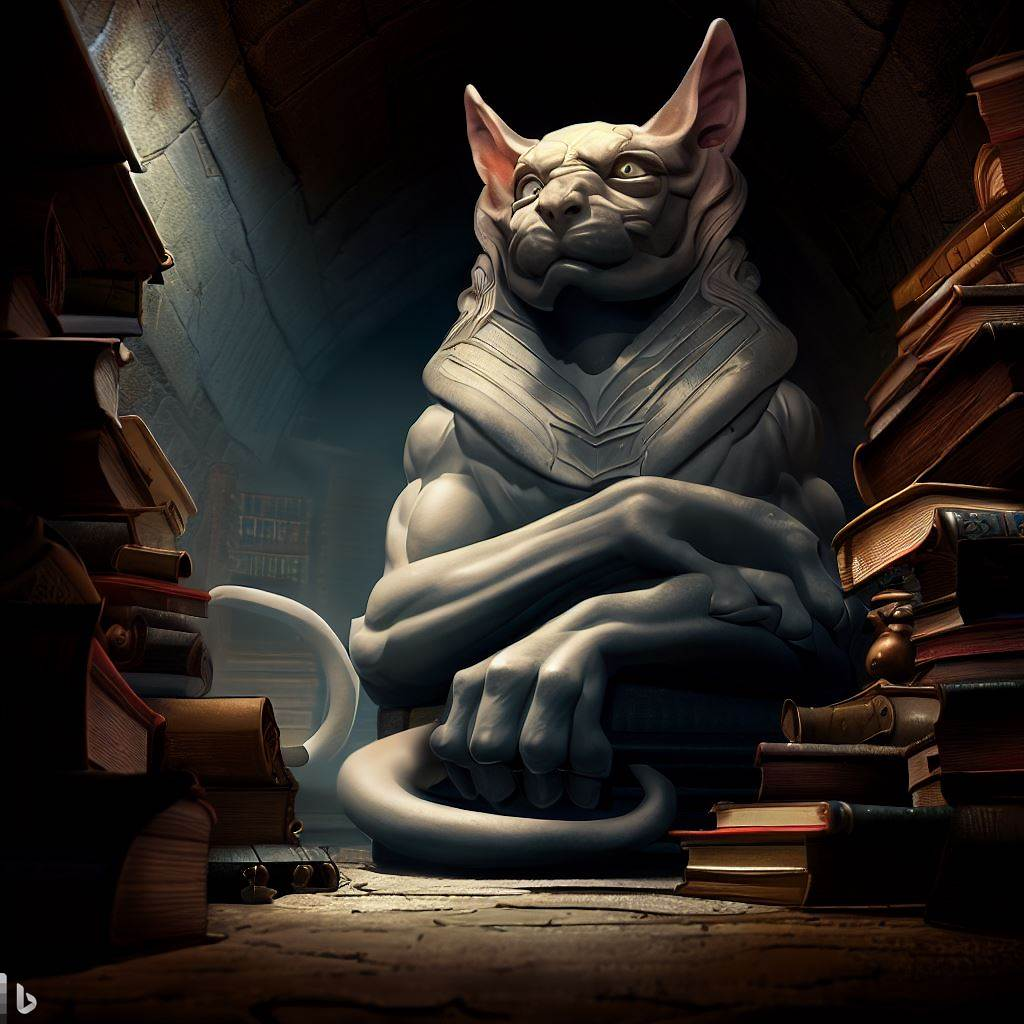
\includegraphics[width=0.99\linewidth]{sphinx2.jpeg}
    \caption{junge Sphinx}
  \end{subfigure}%
  \begin{subfigure}{0.3\textwidth}
    \centering
    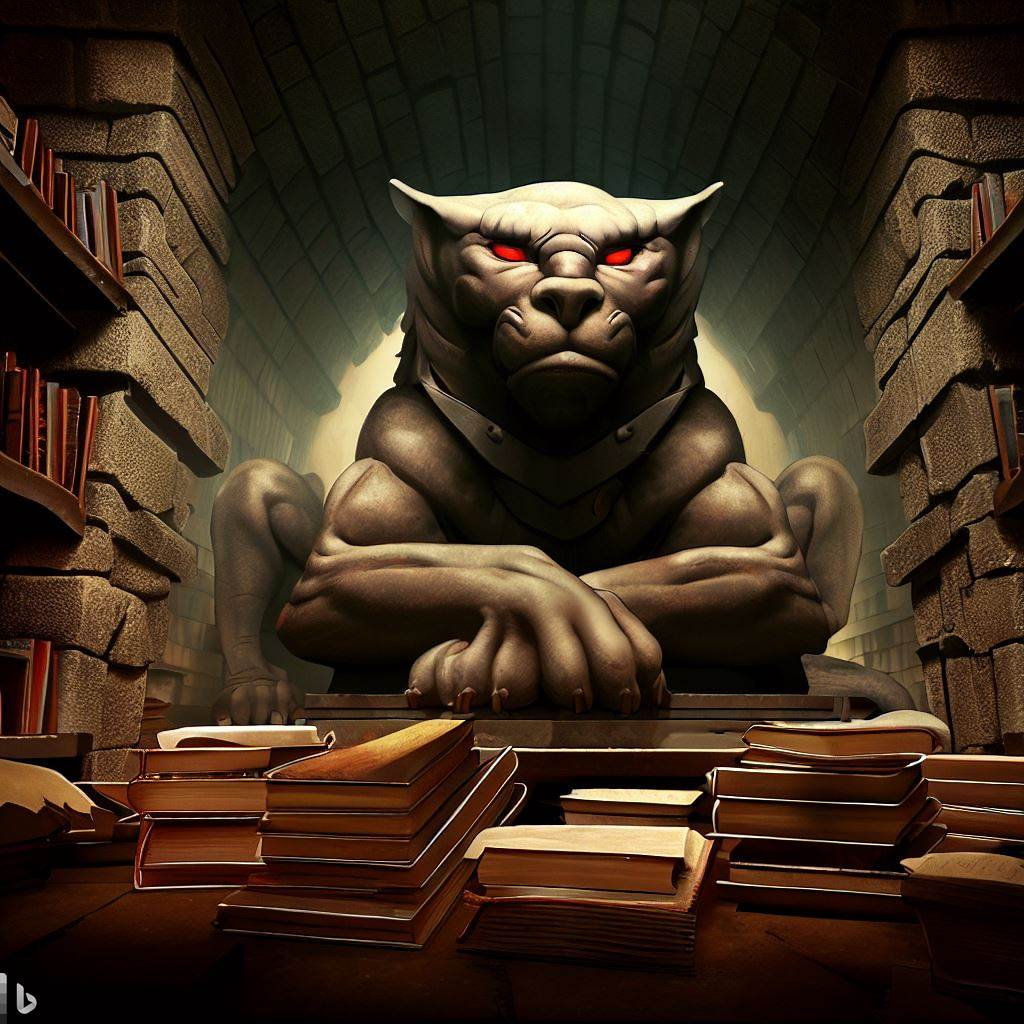
\includegraphics[width=0.99\linewidth]{sphinx3.jpeg}
    \caption{wachsame Sphinx}
  \end{subfigure}
\end{figure}

\subsubsection{Harpyien\label{harpie}}
\label{sec:orgb185d0b}
Im Umland von Astrario gibt es ein verstecktes Harpyien - Lager, bestehend aus 2 Harpyien; sie haben die Körper schöner Jungfrauen, aber Flügel von Geiern und lange Krallen; sie verschleppen Menschen und nehmen ihnen das Essen weg, um sie lange leiden zu sehen; sie zerstören auch mutwillig die Ernten der Menschen; sie fürchten Blasmusik, Gesang und generell Musik - nur dadurch sind sie zu vertreiben bzw. Umzubringen
\begin{figure}[H]
\centering
\caption{Harpyien}
\label{fig:harpie}
  \begin{subfigure}{0.3\textwidth}
    \centering
    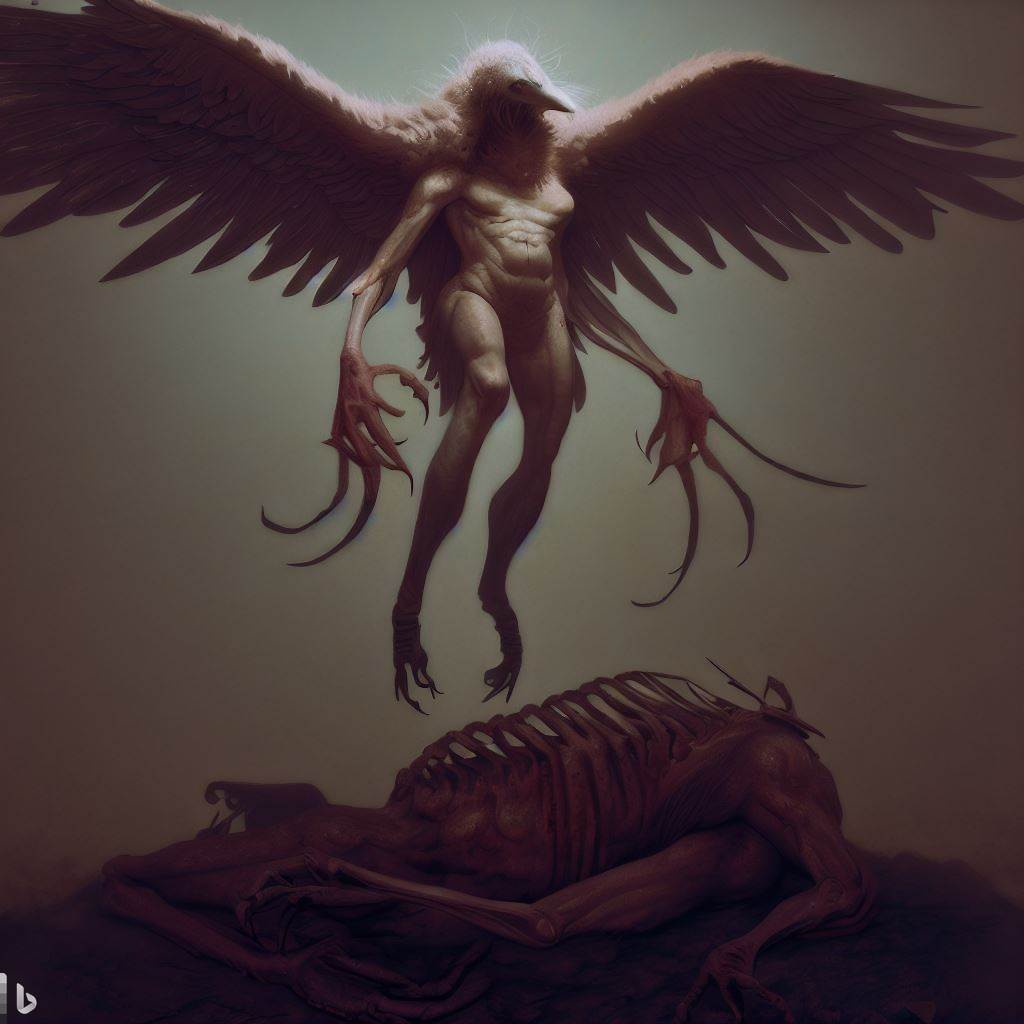
\includegraphics[width=0.99\linewidth]{harpie1.jpeg}
    \caption{alpha Harpie}
  \end{subfigure}%
  \begin{subfigure}{0.3\textwidth}
    \centering
    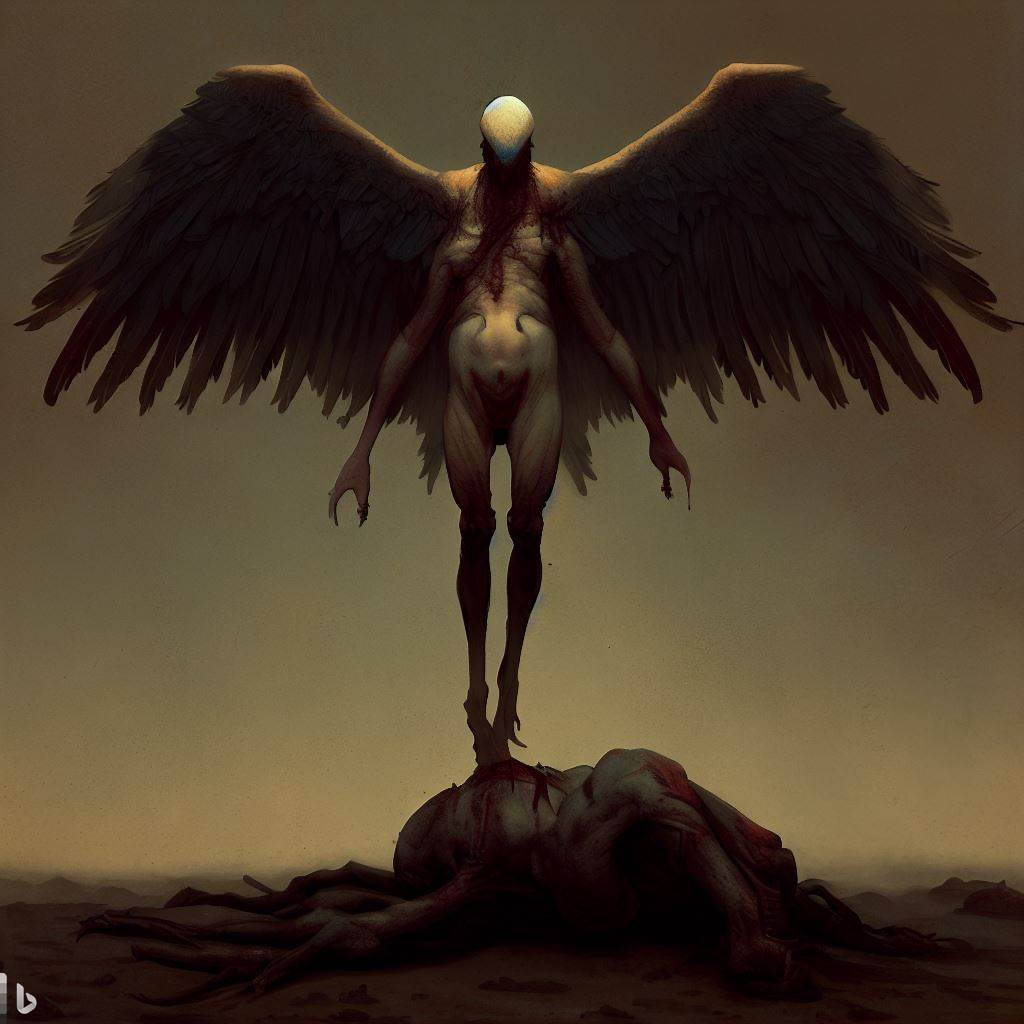
\includegraphics[width=0.99\linewidth]{harpie2.jpeg}
    \caption{gewöhnliche Harpie}
  \end{subfigure}%
\begin{subfigure}{0.3\textwidth}
    \centering
    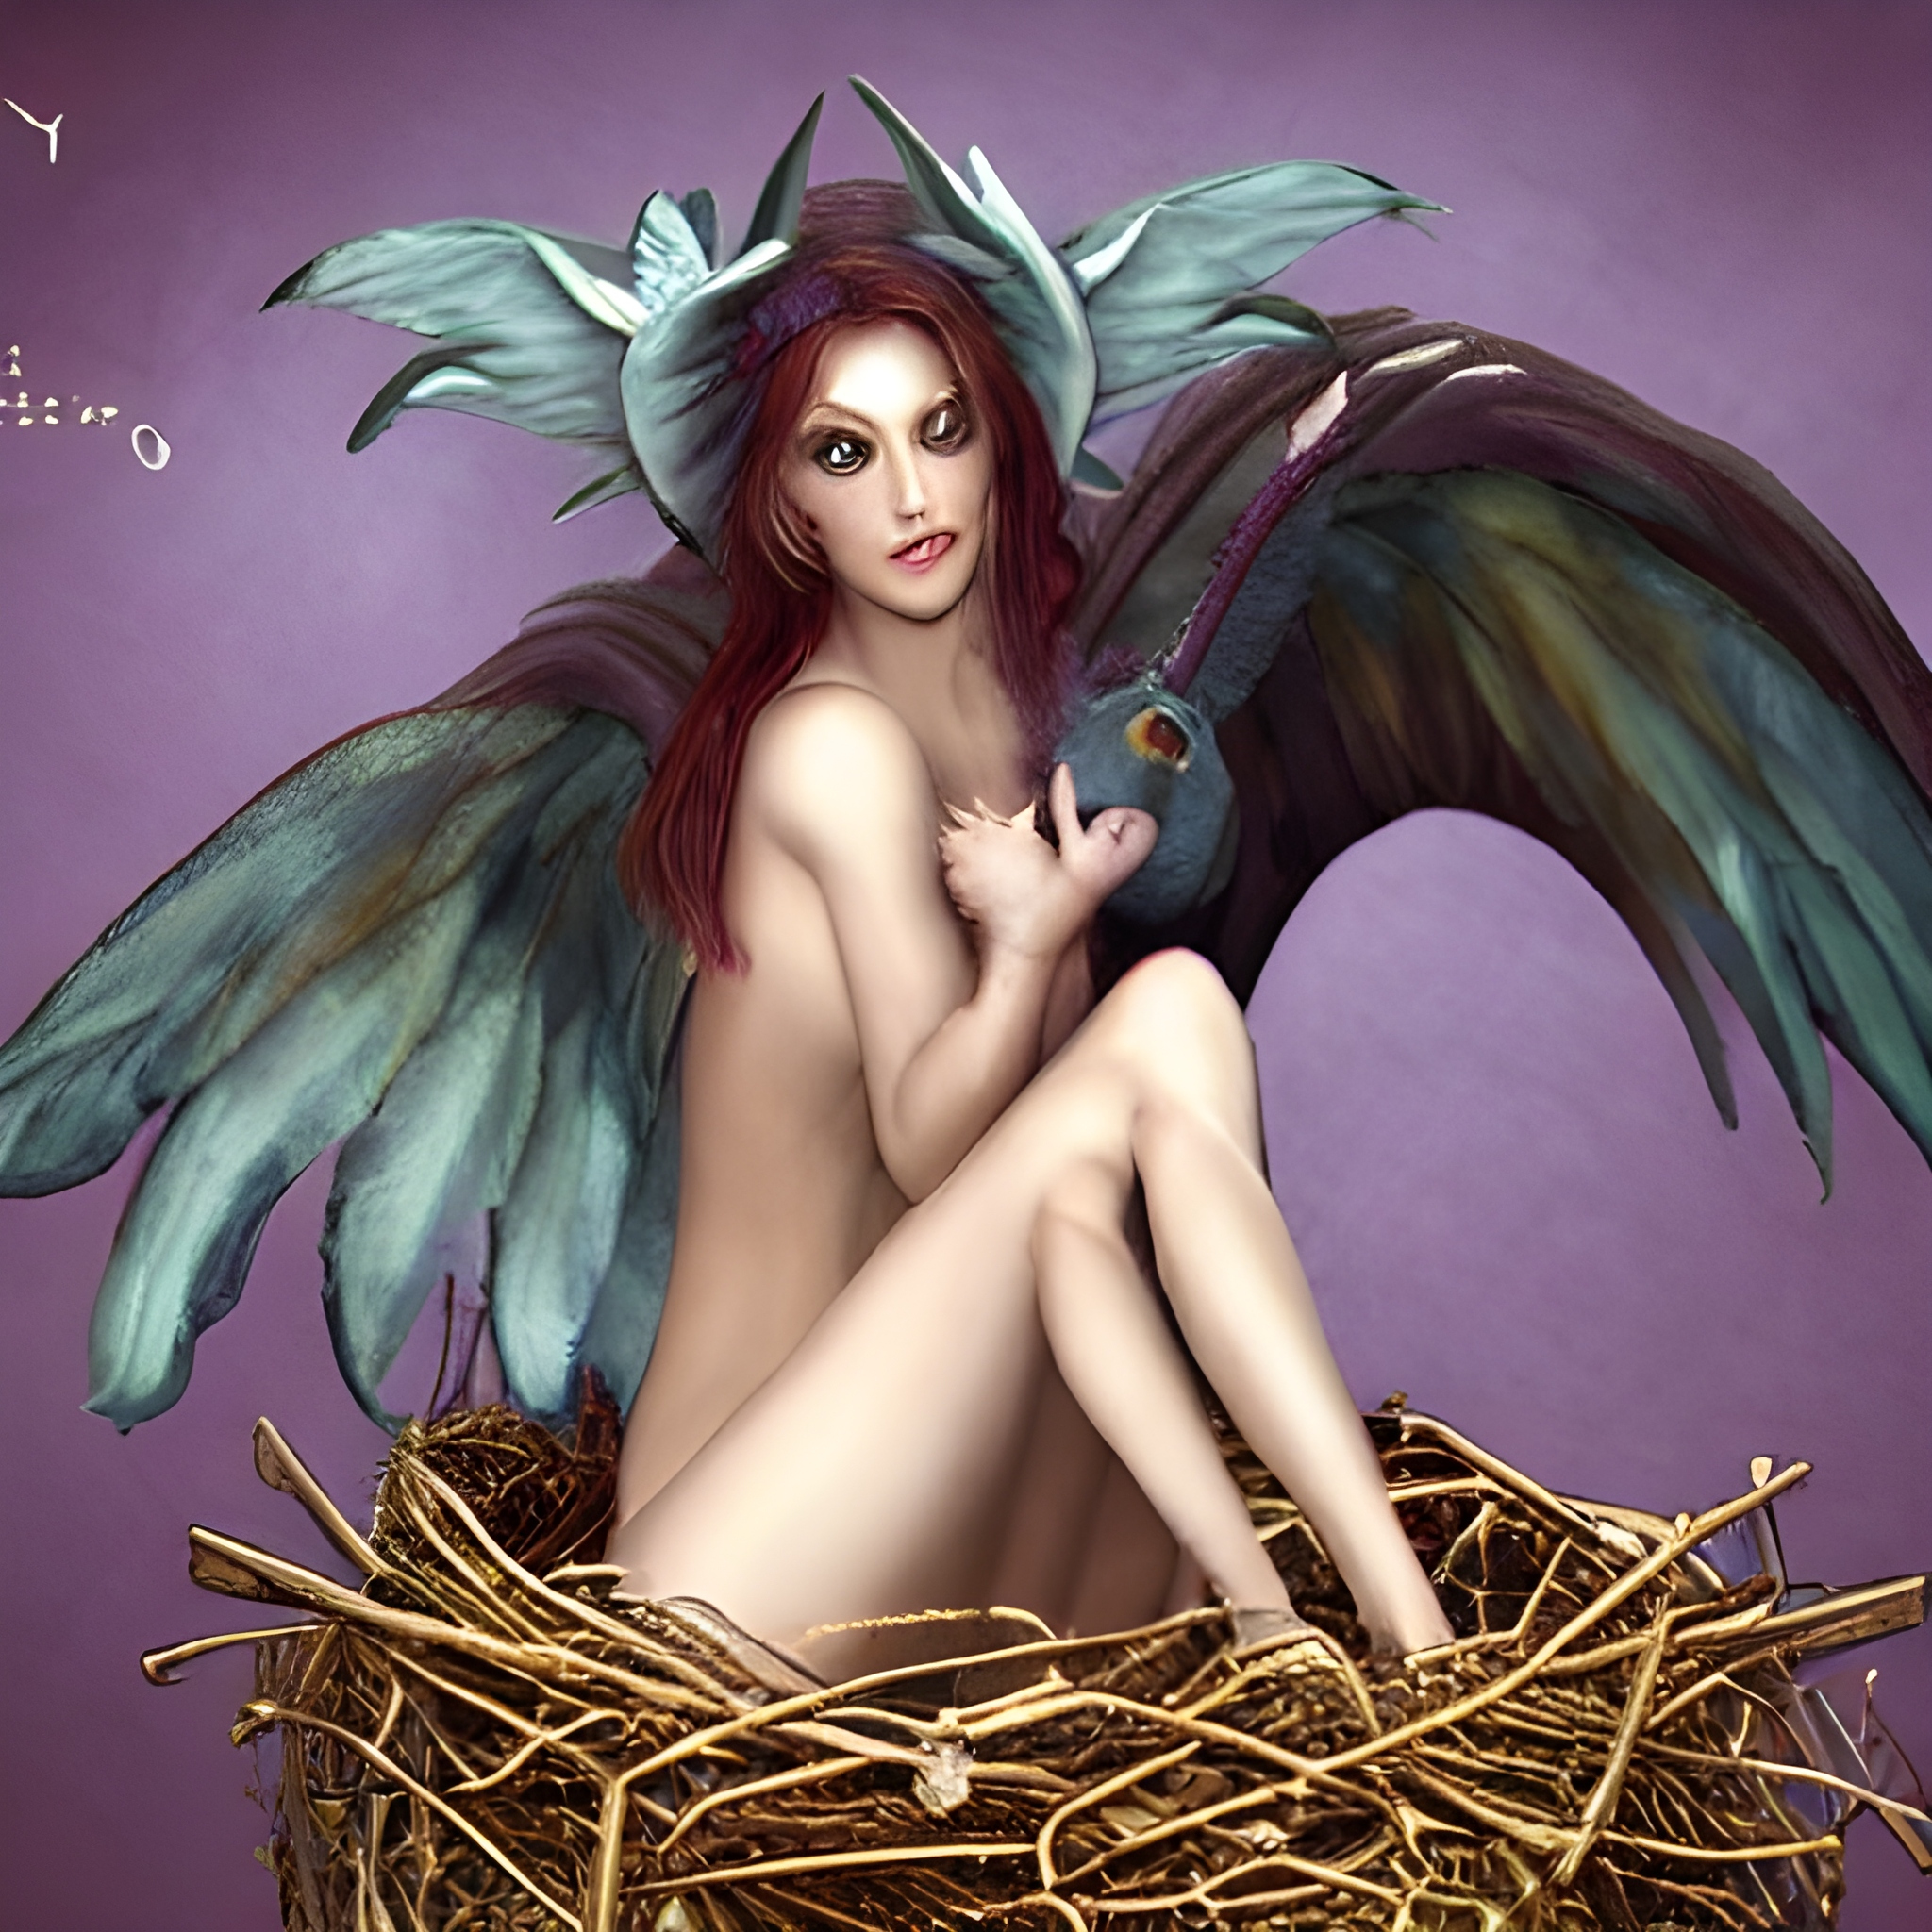
\includegraphics[width=0.99\linewidth]{harpie3.jpeg}
    \caption{schöne Harpie}
  \end{subfigure}
\end{figure}

\subsubsection{Baba Yaga\label{baba}}
\label{sec:org968e80e}
Eine grauenhafte kannibalische Hexe, die am liebsten Kinder verspeist; sie entführt die Kinder Astrario’s; Sie hat keine Beine, sondern ihr Oberkörper steckt in einer Haltevorrichtung, mit der sie springen kann; sie ist sehr langsam und auch sehr laut; schnell bewegen kann sie sich nicht;
\begin{figure}[H]
\centering
\caption{Baba Yaga}
\label{fig:baba}
  \begin{subfigure}{0.5\textwidth}
    \centering
    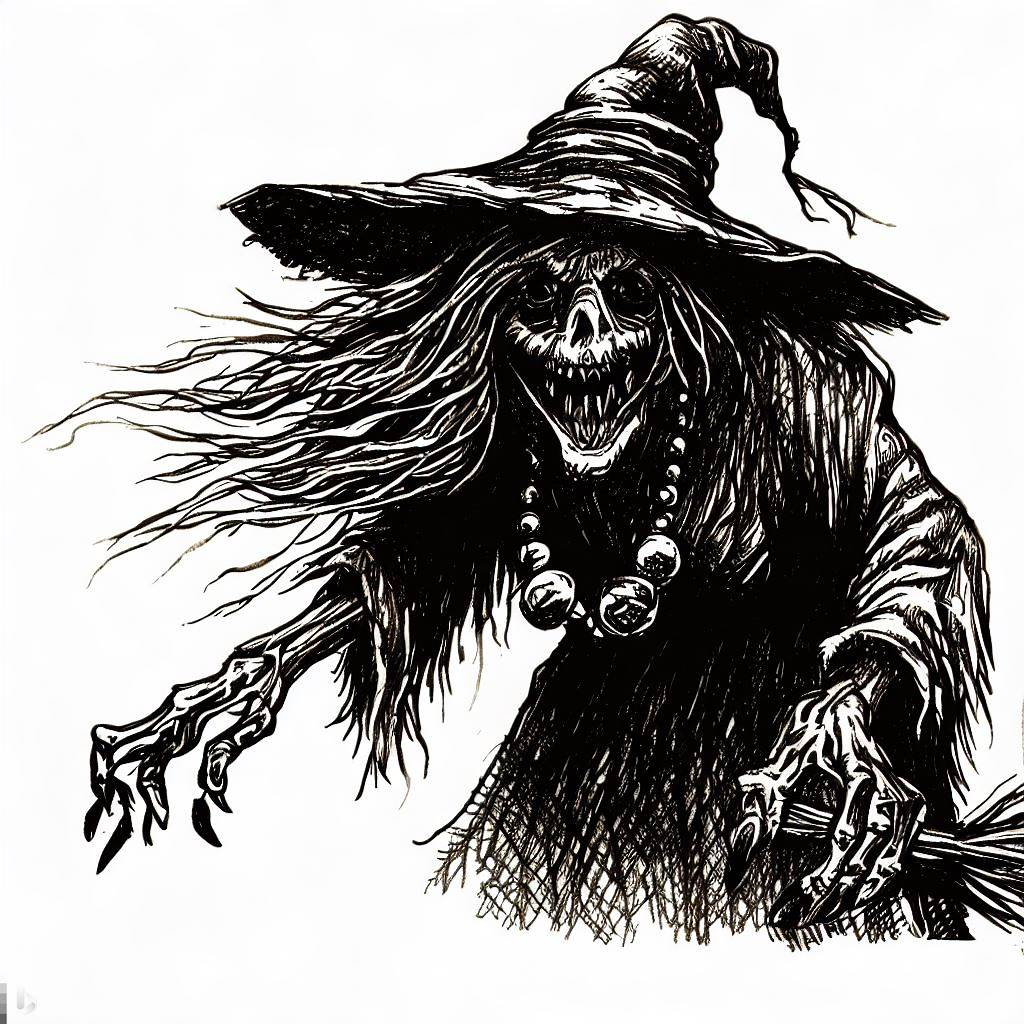
\includegraphics[width=0.8\linewidth]{baba1.jpeg}
    \caption{Zeichnung einer Baba Yaga}
  \end{subfigure}%
  \begin{subfigure}{0.5\textwidth}
    \centering
    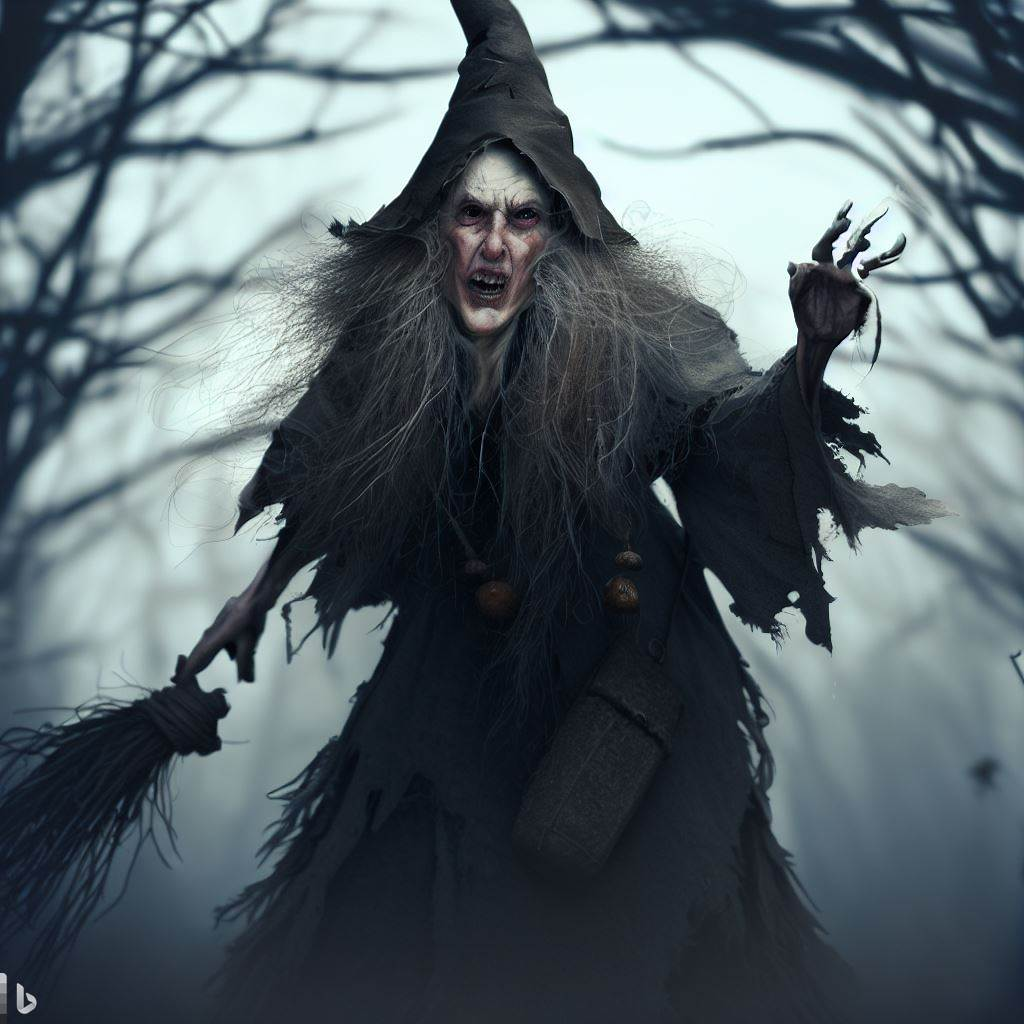
\includegraphics[width=0.8\linewidth]{baba2.jpeg}
    \caption{Baba Yaga}
  \end{subfigure}
\end{figure}

\subsubsection{Buchling\label{buchling}}
\label{sec:org8183721}
Kleine grüne Zyklopen.
\begin{figure}[H]
\centering
\caption{Buchlinge}
    \label{fig:buchling}
  \begin{subfigure}{0.5\textwidth}
    \centering
    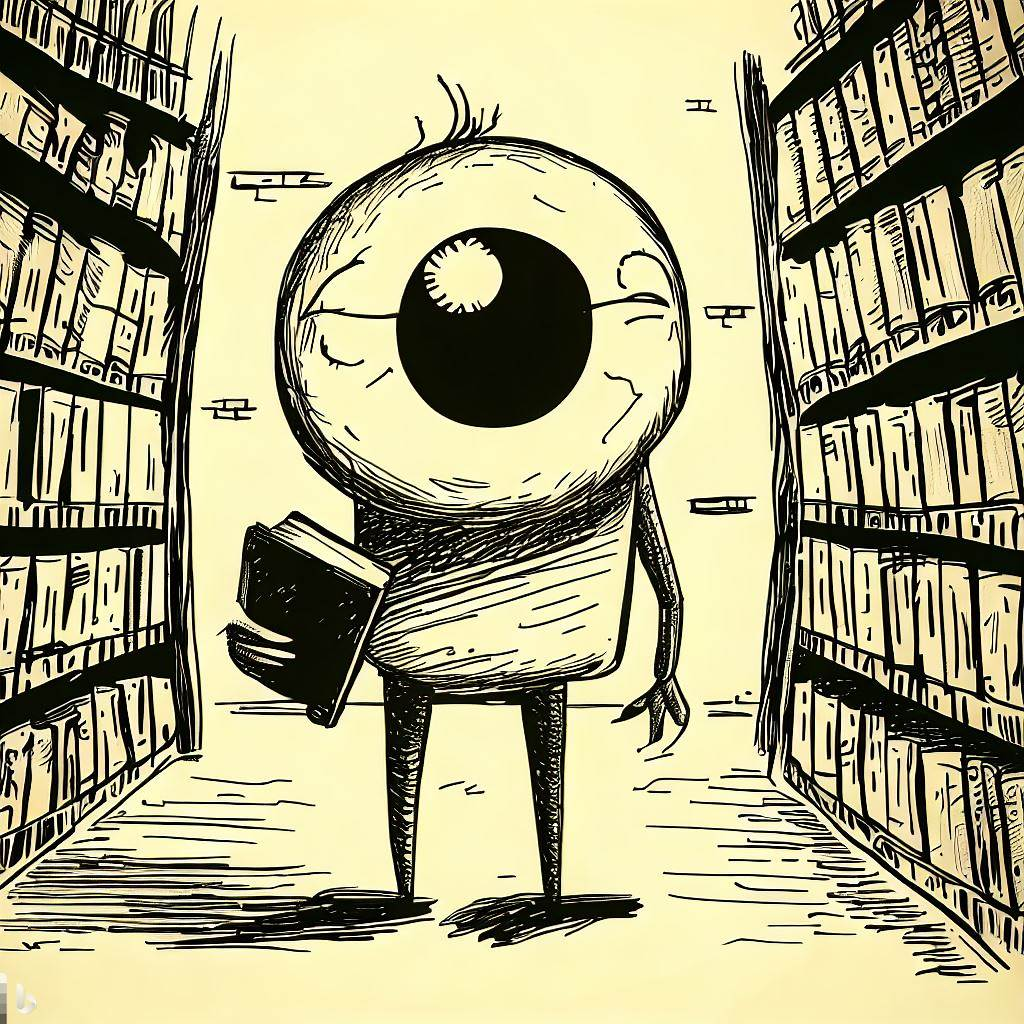
\includegraphics[width=0.8\linewidth]{buchling1.jpeg}
    \caption{ein Buchling}
  \end{subfigure}%
  \begin{subfigure}{0.5\textwidth}
    \centering
    
\includegraphics[width=0.8\linewidth]{buchling2.jpeg}
    \caption{ein anderer Buchling}
  \end{subfigure}
\end{figure}

\newpage

\subsection{Weitluftebene}
\label{sec:orga0ec355}
\subsubsection{Wasserpferde\label{seahorse}}
\label{sec:org467f283}
Vor diesen mythischen Wesen sollte ein großer Bogen gemacht werden - sie beherrschen sowohl Wasser als auch Eis und mögen keine Fremden. Steigt jemand auf seinen Rücken, wird es in die Tiefen des Wassers gezogen und stirbt an einem qualvollen Tod. Gelingt es einem Abenteurer, das Tier - mit Sanftmut und Güte - zu zähmen oder erachtet es eine Person als würdig und reinen Herzens, so wird es zum lebenslangen Begleiter. Es kann Sachen für seine Besitzer tragen, sie mit Wasser versorgen oder bei großer Hitze etwas abkühlen. Es kann auch Wasser zu Eis umwandeln und dadurch geschickt im Kampf eingesetzt werden.
\begin{figure}[H]
\centering
\caption{Wasserpferd}
\label{fig:wasserpferd}
  \begin{subfigure}{0.3\textwidth}
    \centering
    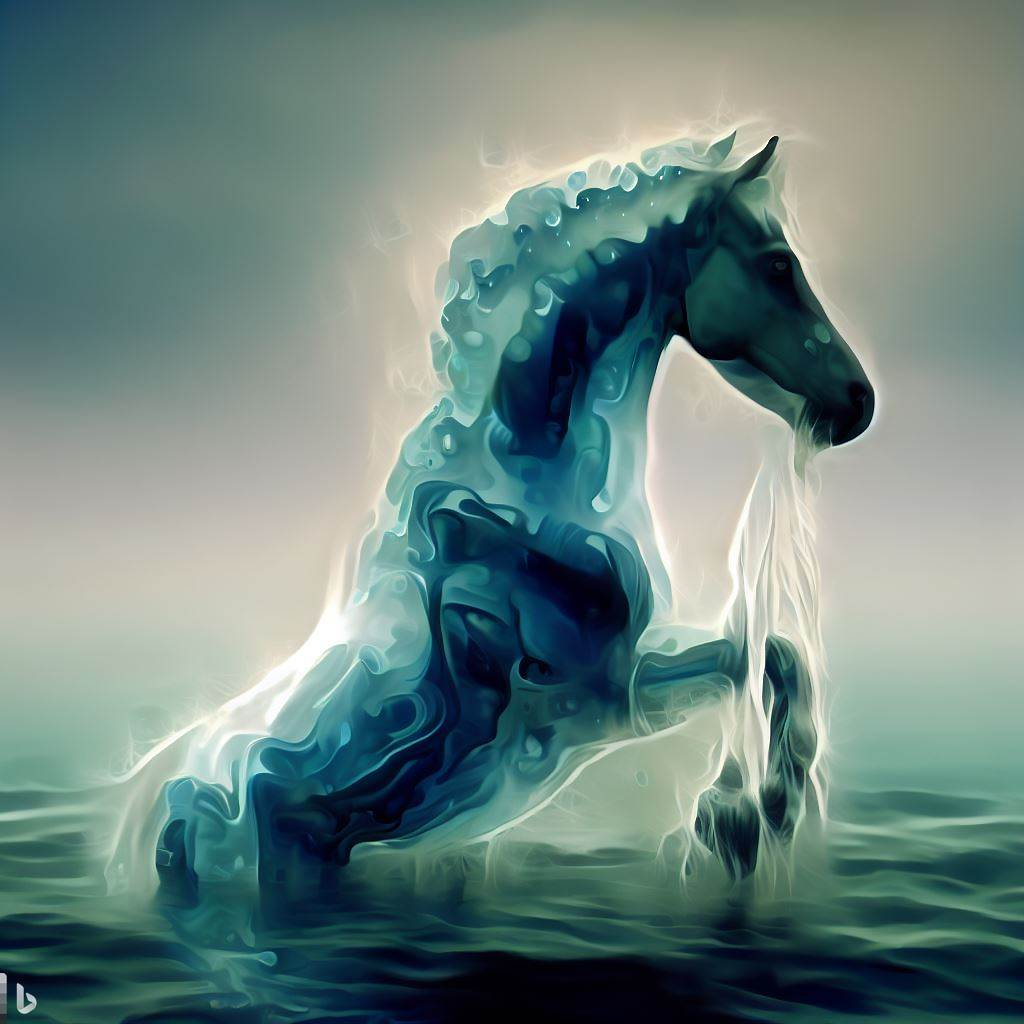
\includegraphics[width=0.99\linewidth]{wasserpferd1.jpeg}
    %\caption{Ethera}
  \end{subfigure}%
  \begin{subfigure}{0.3\textwidth}
    \centering
    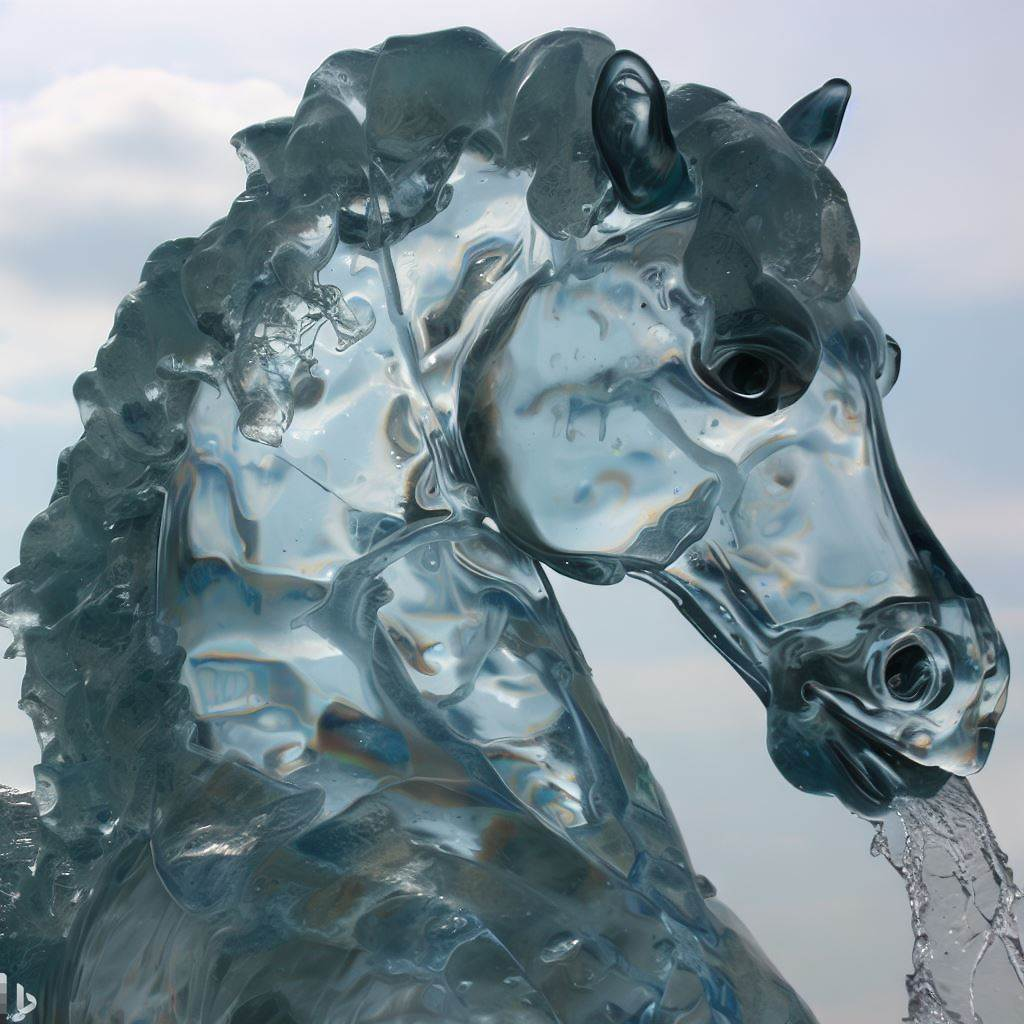
\includegraphics[width=0.99\linewidth]{wasserpferd2.jpeg}
    %\caption{Etherus Meister}
  \end{subfigure}%
  \begin{subfigure}{0.3\textwidth}
    \centering
    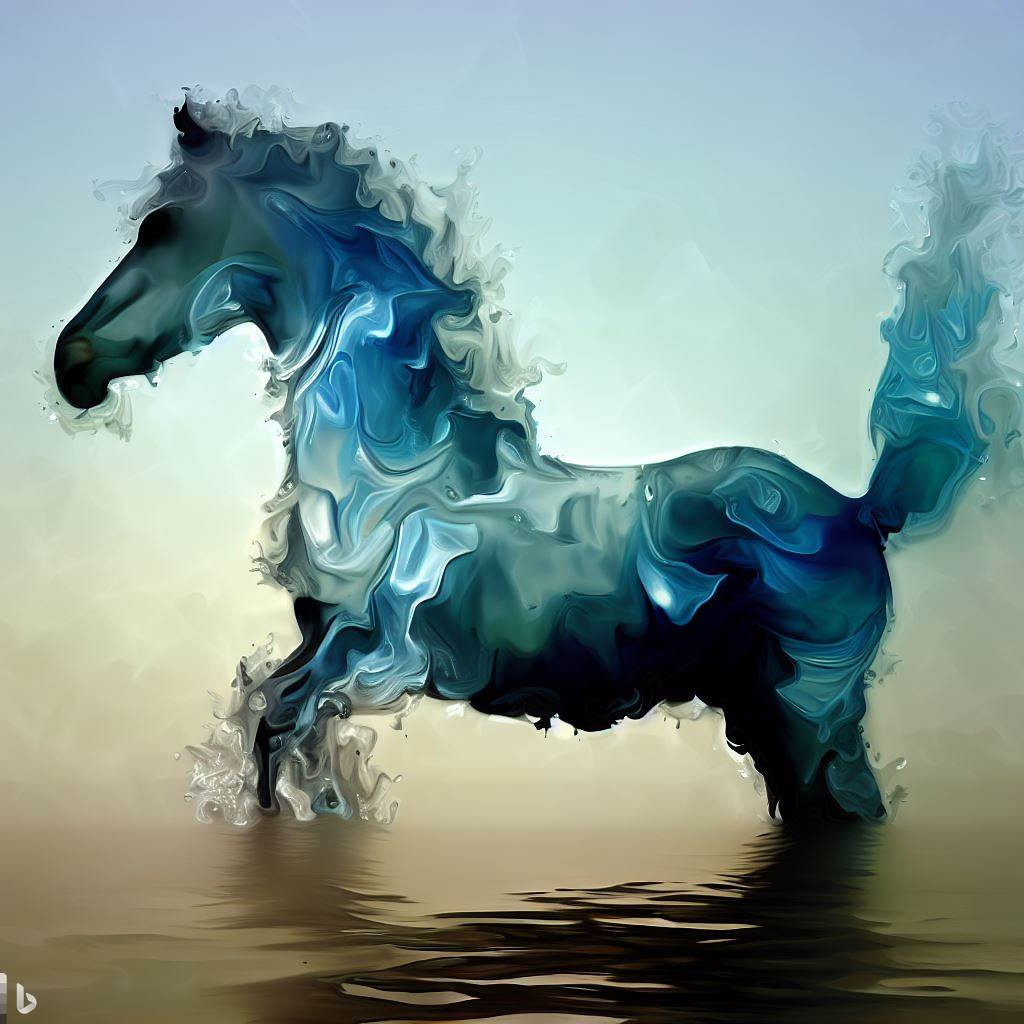
\includegraphics[width=0.99\linewidth]{wasserpferd3.jpeg}
    %\caption{Etherus Schüler}
  \end{subfigure}
\end{figure}

\subsubsection{Hydra\label{hydra}}
\label{sec:org8e04679}
Eine Schlange mit mehreren Köpfen (bis zu ca. 5 Köpfen - 1 Kopf pro Spieler), ein sehr gefährliches Wesen, das Gegner beißt und vergiftet; sehr aggressiv - sollte besser umgangen werden
\begin{figure}[H]
\centering
\caption{Hydra}
\label{fig:hydra}
  \begin{subfigure}{0.3\textwidth}
    \centering
    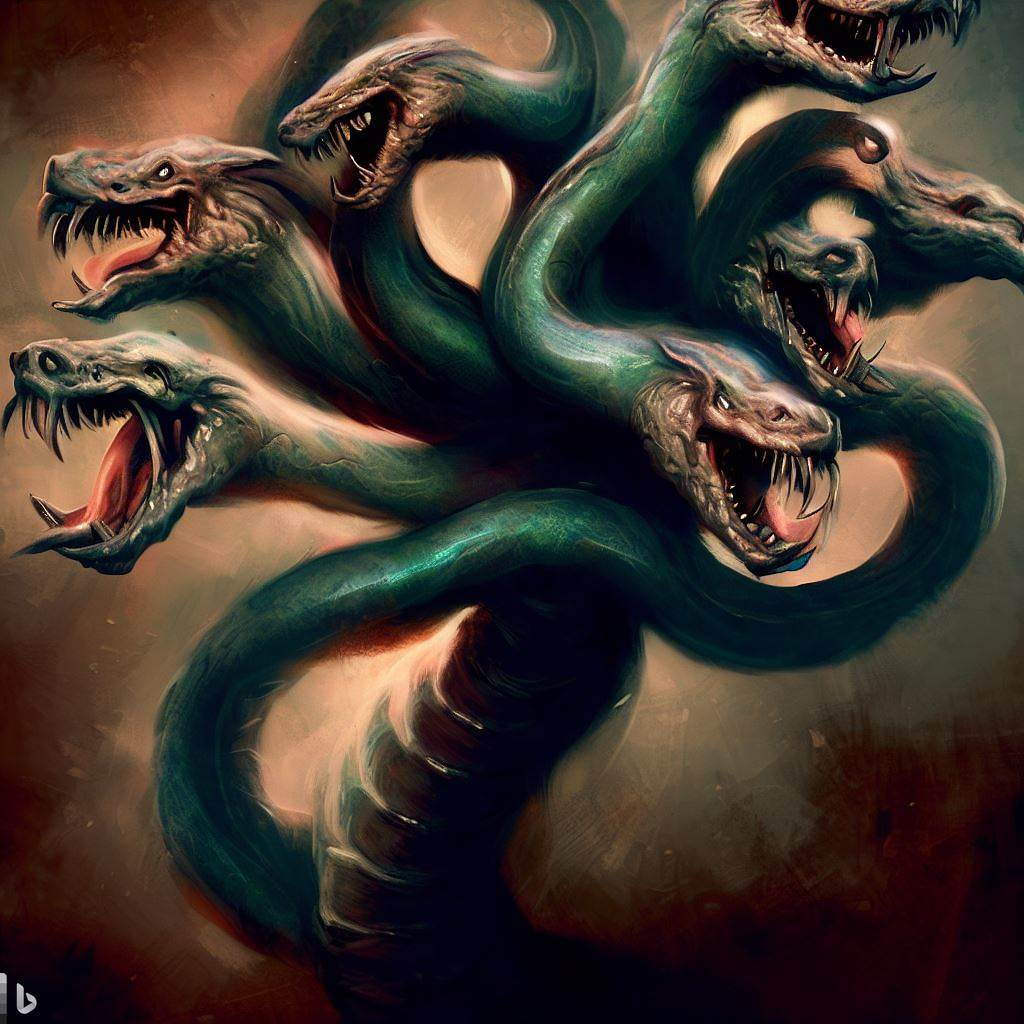
\includegraphics[width=0.99\linewidth]{hydra1.jpeg}
    %\caption{Ethera}
  \end{subfigure}%
  \begin{subfigure}{0.3\textwidth}
    \centering
    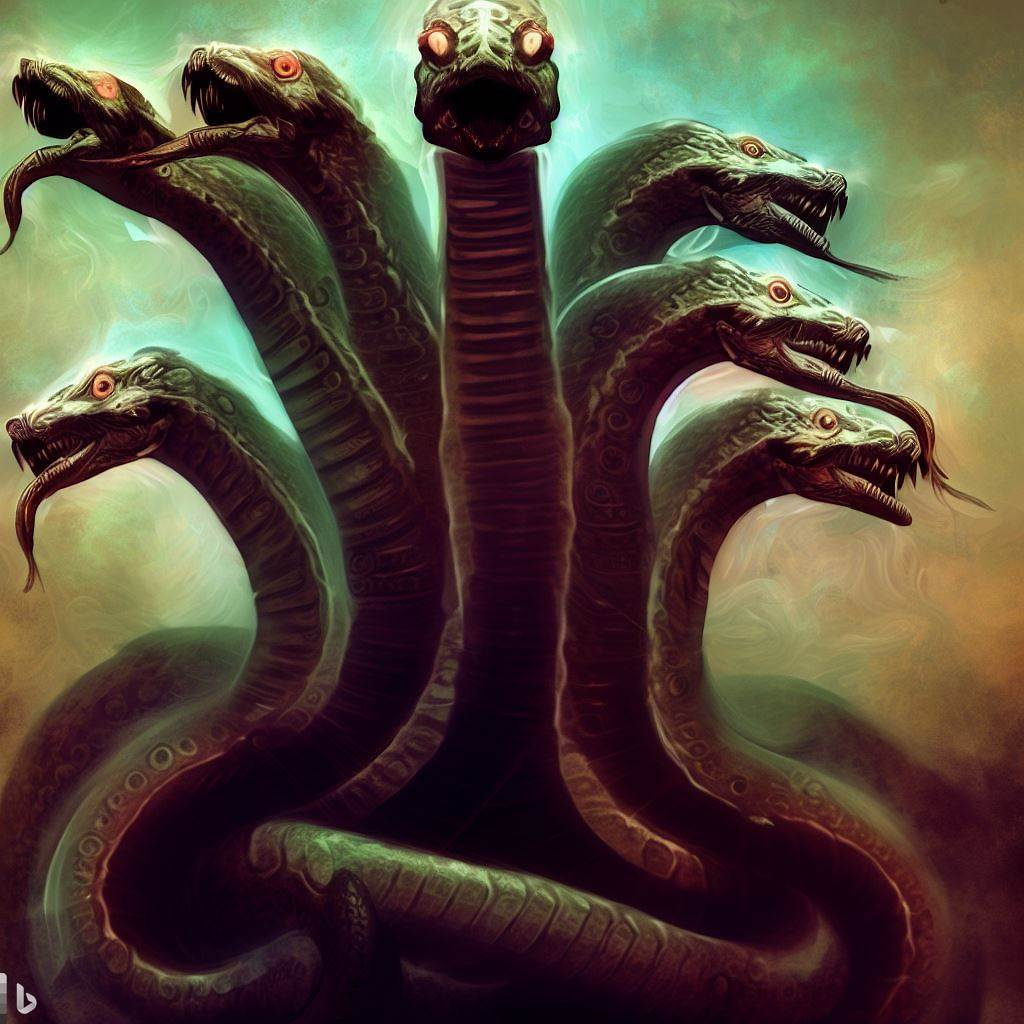
\includegraphics[width=0.99\linewidth]{hydra2.jpeg}
    %\caption{Etherus Meister}
  \end{subfigure}%
  \begin{subfigure}{0.3\textwidth}
    \centering
    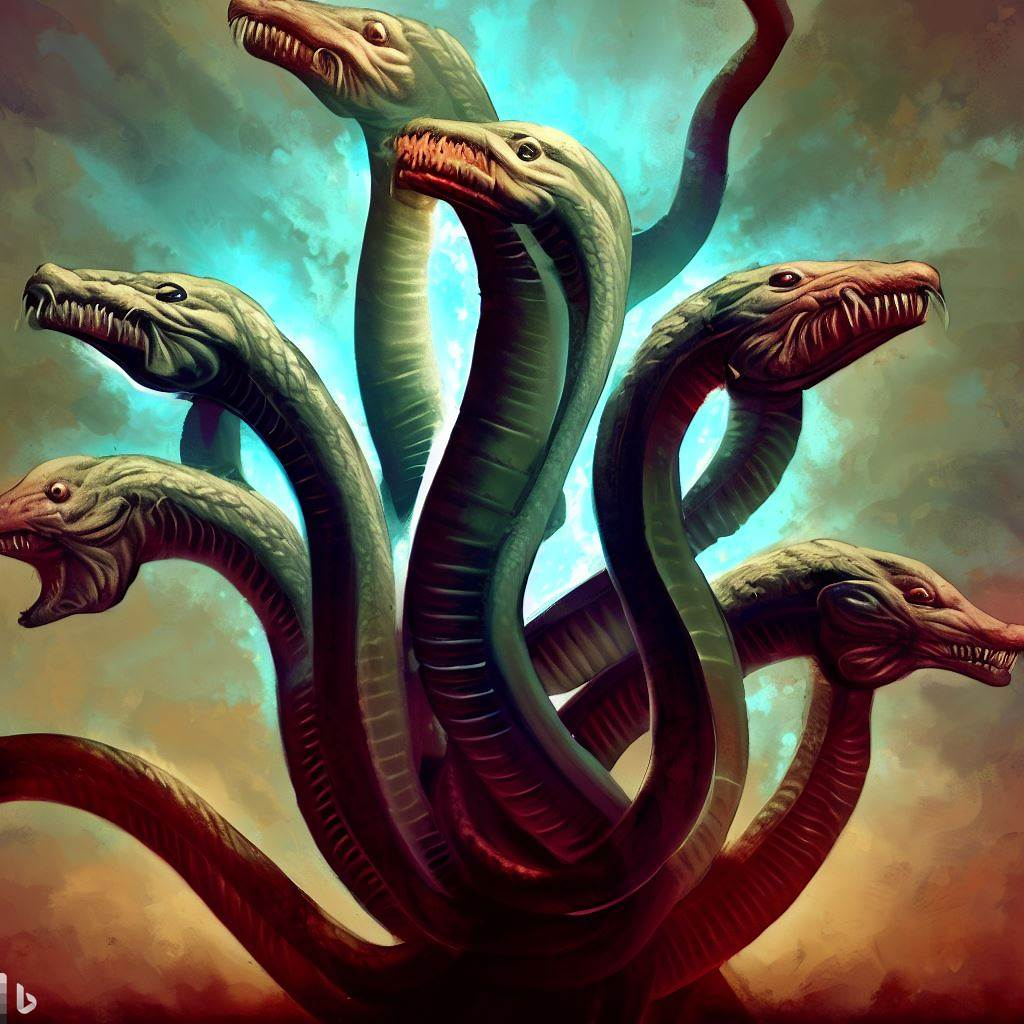
\includegraphics[width=0.99\linewidth]{hydra3.jpeg}
    %\caption{Etherus Schüler}
  \end{subfigure}
\end{figure}

\newpage

\subsection{Eversonn}
\label{sec:org2c18137}
\subsubsection{Phönix\label{phönix}}
\label{sec:org1ed6fdc}
nur in Eversonn können Phönixe am Himmel beobachtet werden; sie sind sehr sanfte und friedliebende Tiere; bittet man sie höflich um Hilfe, gewähren sie der Person 3 Phönixtränen - mit diesen können tote Personen wiederbelebt werden und werden vollständig geheilt; Phönixe sind sehr intelligent und geben ihre Tränen nicht ohne weiteres her, man muss sie schon in ein gutes Gespräch verwickeln;
\begin{figure}[H]
\centering
\caption{Phönix}
\label{fig:phoenix}
  \begin{subfigure}{0.3\textwidth}
    \centering
    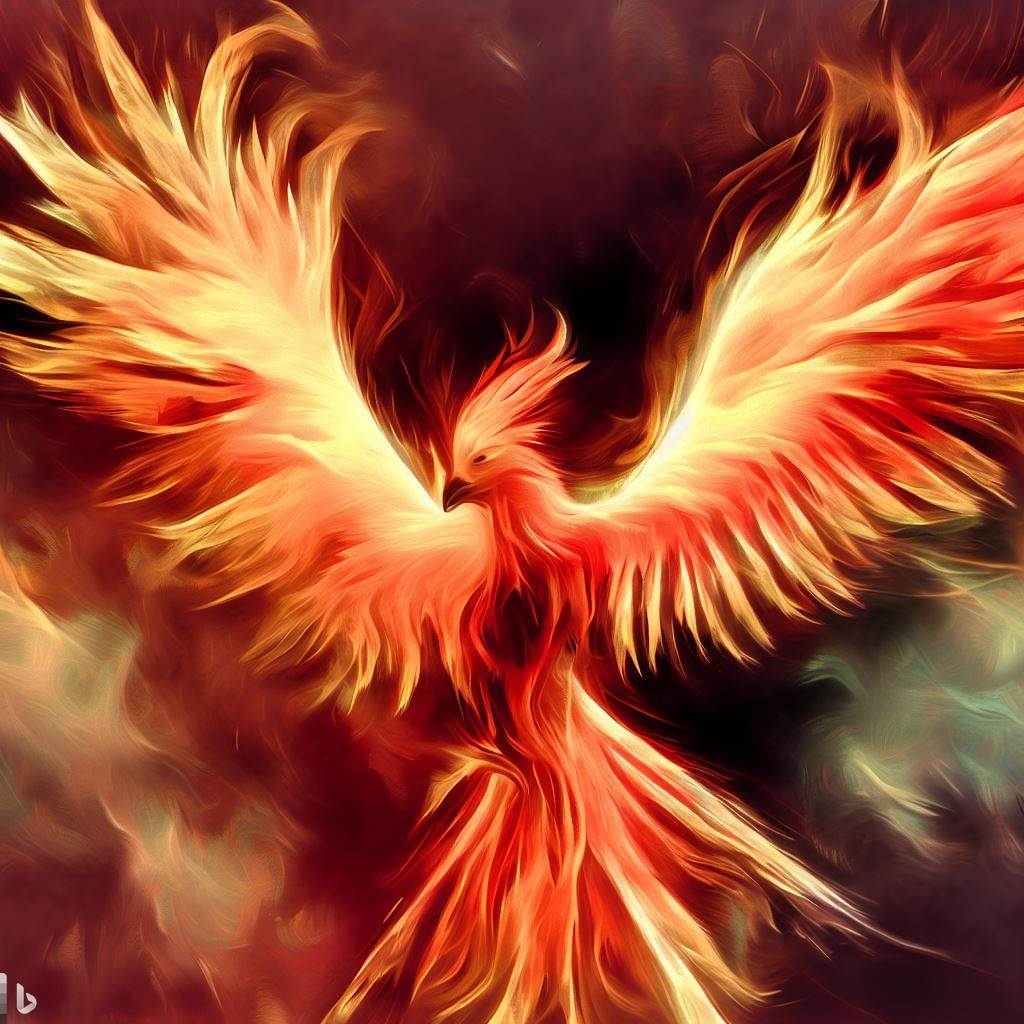
\includegraphics[width=0.99\linewidth]{phoenix1.jpeg}
    %\caption{Ethera}
  \end{subfigure}%
  \begin{subfigure}{0.3\textwidth}
    \centering
    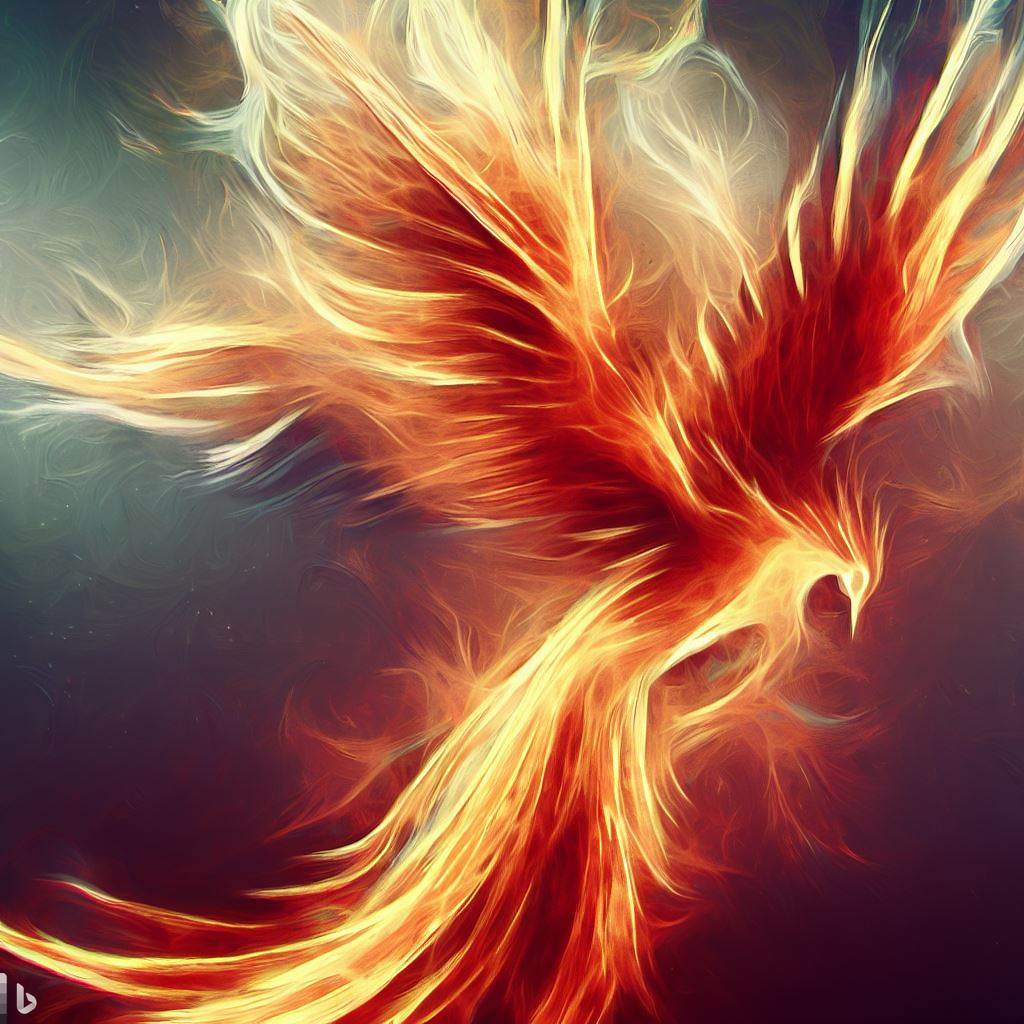
\includegraphics[width=0.99\linewidth]{phoenix2.jpeg}
    %\caption{Etherus Meister}
  \end{subfigure}%
  \begin{subfigure}{0.3\textwidth}
    \centering
    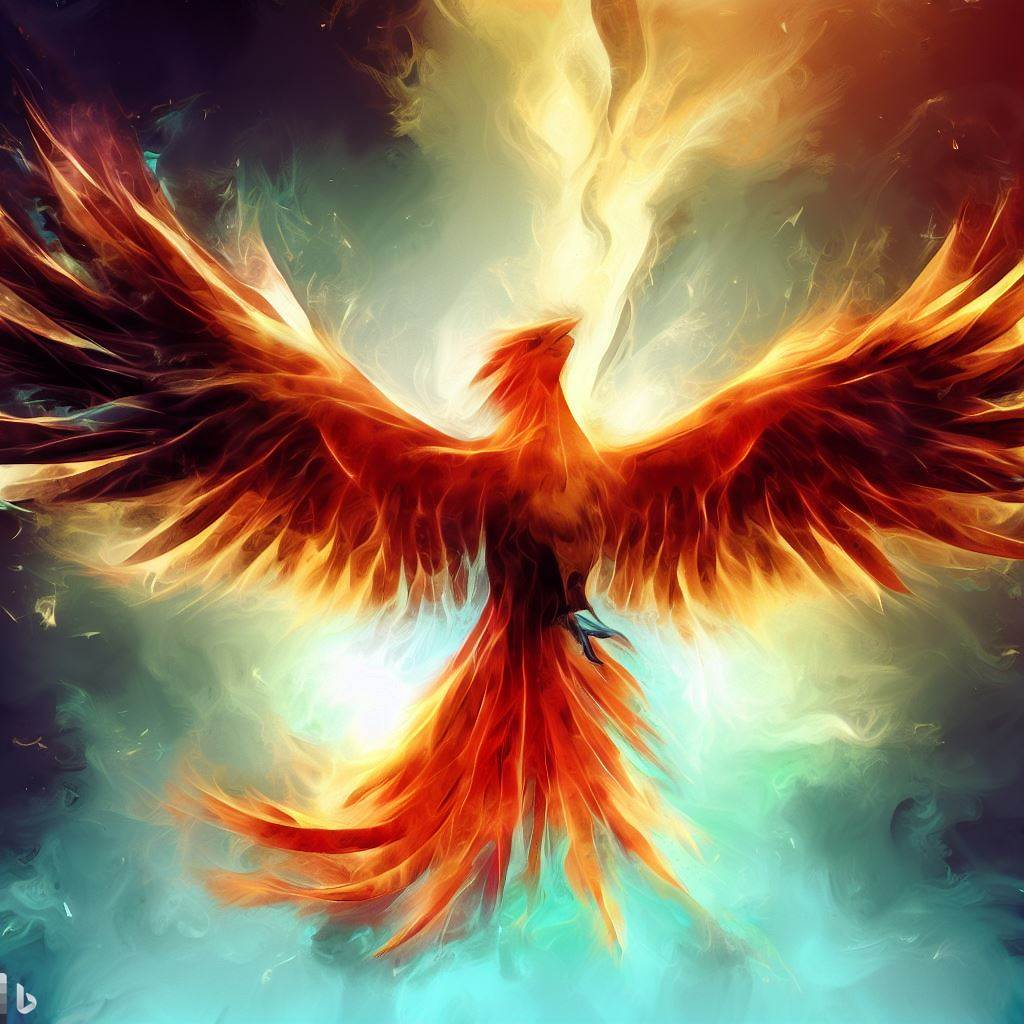
\includegraphics[width=0.99\linewidth]{phoenix3.jpeg}
    %\caption{Etherus Schüler}
  \end{subfigure}
\end{figure}

\newpage

\subsection{Höhle der Erinnerung}
\label{sec:org3ce0398}
\subsubsection{Drache der Weisheit\label{wdrache}}
\label{sec:org8960083}
ein chinesischer, goldener Drache; spricht sehr eloquent und wortgewandt, ist sehr weise und lebenserfahren und ist Lebewesen gegenüber gut gesinnt, wenn sie ihn nicht umbringen möchten; schläft tief im innersten der Höhle und verlässt sie ein paar Mal täglich, um zu fliegen; ist Wächter der Perle der Weisheit - gibt sie unter keinen Umständen her;
\begin{figure}[H]
\centering
\caption{Drache der Weisheit}
\label{fig:drache}
  \begin{subfigure}{0.3\textwidth}
    \centering
    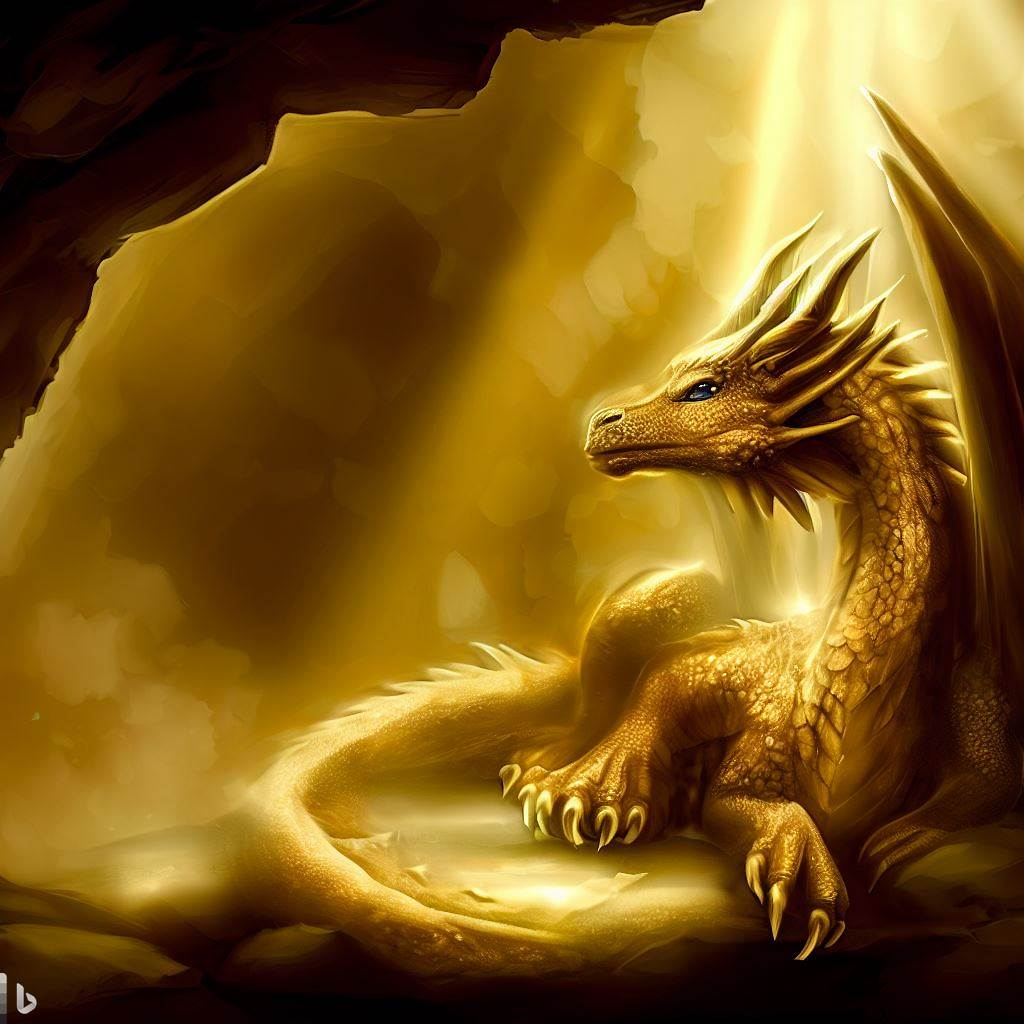
\includegraphics[width=0.99\linewidth]{drache1.jpeg}
    %\caption{Ethera}
  \end{subfigure}%
  \begin{subfigure}{0.3\textwidth}
    \centering
    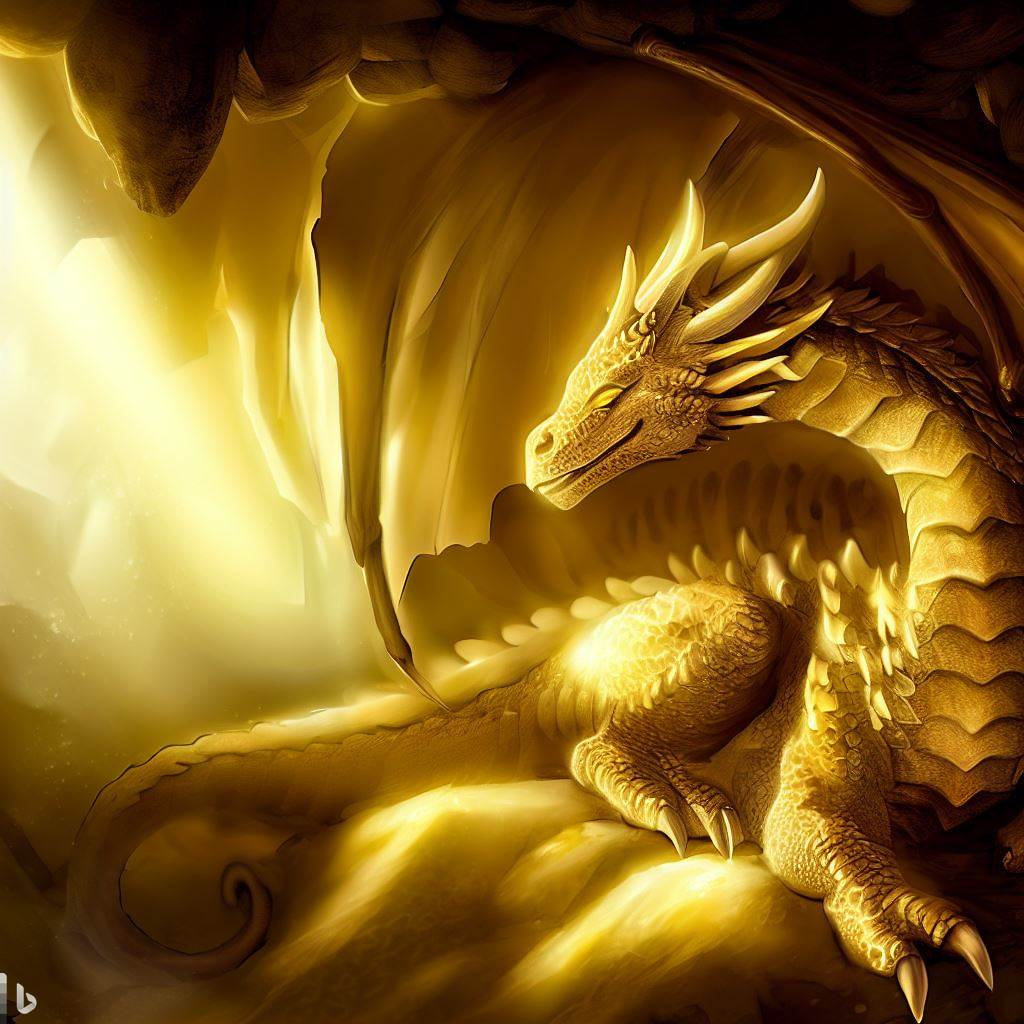
\includegraphics[width=0.99\linewidth]{drache2.jpeg}
    %\caption{Etherus Meister}
  \end{subfigure}%
  \begin{subfigure}{0.3\textwidth}
    \centering
    \includegraphics[width=0.99\linewidth]{drache3.jpeg}
    %\caption{Etherus Schüler}
  \end{subfigure}
\end{figure}

\newpage

\subsection{Tal der Schatten}
\label{sec:orgbeb03eb}
\subsubsection{Garuda\label{garuda}}
\label{sec:orga70815e}
Dies ist ein Riesenvogel, der eine Mischung als Vogel und Mensch darstellt. Er fliegt über das Tal und sollte nicht herausgefordert werden; er greift nicht ohne Grund an; im Grunde ist er ein Dämon, der Bringer des Lebens und Überbringer von Wissen; Er hilft den Lebewesen des Tals, frisst aber Menschen.
\begin{figure}[H]
\centering
\caption{Garuda}
\label{fig:garuda}
  \begin{subfigure}{0.3\textwidth}
    \centering
    \includegraphics[width=0.99\linewidth]{garuda1.jpeg}
    %\caption{Ethera}
  \end{subfigure}%
  \begin{subfigure}{0.3\textwidth}
    \centering
    \includegraphics[width=0.99\linewidth]{garuda2.jpeg}
    %\caption{Etherus Meister}
  \end{subfigure}%
  \begin{subfigure}{0.3\textwidth}
    \centering
    \includegraphics[width=0.99\linewidth]{garuda3.jpeg}
    %\caption{Etherus Schüler}
  \end{subfigure}
\end{figure}

\subsubsection{Chimäre\label{chimäre}}
\label{sec:org1b685b1}
Kopf eines Löwen, Körper einer Ziege; frisst alles, was ihm in die Quere kommt und spuckt Feuer; hat noch einen Vater - eine Chimäre mit 3 Köpfen!
\begin{figure}[H]
\centering
\caption{Chimäre}
\label{fig:chim}
  \begin{subfigure}{0.3\textwidth}
    \centering
    \includegraphics[width=0.99\linewidth]{chim1.jpeg}
    %\caption{Ethera}
  \end{subfigure}%
  \begin{subfigure}{0.3\textwidth}
    \centering
    \includegraphics[width=0.99\linewidth]{chim2.jpeg}
    %\caption{Etherus Meister}
  \end{subfigure}%
  \begin{subfigure}{0.3\textwidth}
    \centering
    \includegraphics[width=0.99\linewidth]{chim3.jpeg}
    %\caption{Etherus Schüler}
  \end{subfigure}
\end{figure}

\newpage
\appendix
\listoffigures
\newpage

\section{Software}
\label{sec:org0494932}
\begin{itemize}
\item Emacs + org-mode (\href{https://orgmode.org/}{https://orgmode.org/})
\item \LaTeX
\item Image Creator from Microsoft Bing (\href{https://www.bing.com/images/create}{https://www.bing.com/images/create})
\item Nortantis fantasy map generator (\href{https://github.com/jeheydorn/nortantis}{https://github.com/jeheydorn/nortantis})
\item Dungeon Scrawl (\href{https://app.dungeonscrawl.com/}{https://app.dungeonscrawl.com/})
\end{itemize}

\section{Inspiration}
\label{sec:orgc402ebd}
\begin{itemize}
\item Der Herr der Ringe
\item Warhammer 40.000
\item The Witcher (Bücher)
\item Harry Potter
\item Walter Moers: Zamonien
\item griechische/römische Mythologie
\end{itemize}
\end{document}